% ============================================================
% CHƯƠNG 3 — QUẢNG BÁ VÀ CHIẾN LƯỢC TIẾP CẬN THỊ TRƯỜNG
% ============================================================
% Phân công tổng hợp (PA3-06):
%   Tổng hợp LaTeX/format : Nguyễn Ngọc Cảnh
%   Kiểm tra logic tổng thể: Nguyễn Anh Thư
%   Kiểm tra marketing     : Trần Minh Quang
%   Kiểm tra số liệu       : Nguyễn Công Toàn
%   Kiểm tra luồng tracking: Lê Nguyên Nhật
% ============================================================

\section{Quảng bá và chiến lược tiếp cận thị trường}

% --- PA3-02 | Nguyễn Anh Thư ---
% ============================================================
% PHẦN 3.1 — MỤC TIÊU QUẢNG BÁ TRONG GIAI ĐOẠN ĐẦU
% ------------------------------------------------------------
% Thuộc: PA3-02
% Người phụ trách chính: Nguyễn Anh Thư – CEO/Project Lead
% Phối hợp: Trần Minh Quang
%
% CÂU HỎI CẦN TRẢ LỜI:
%   - Trong giai đoạn đầu, 1Stream muốn khách hàng biết, tin hay thực hiện hành động gì?
%   - Lời kêu gọi hành động chính là gì? (Đăng ký demo / tư vấn / video mẫu / pilot)
%
% OUTPUT BẮT BUỘC:
%   - Mục tiêu quảng bá rõ ràng cho giai đoạn pre-launch và launch
%   - CTA chính và CTA phụ
% ============================================================

\subsection{Mục tiêu quảng bá trong giai đoạn đầu}

% TODO (Nguyễn Anh Thư): Viết nội dung mục 3.1
% Gợi ý cấu trúc:
%   1. Mục tiêu theo giai đoạn (trước ra mắt / tuần ra mắt / sau ra mắt)
%   2. Ưu tiên: Nhận biết → Quan tâm → Hành động (đăng ký pilot)
%   3. CTA chính: Đăng ký pilot / Đặt lịch demo
%   4. Giới hạn: Không quảng bá tính năng chưa hoàn thiện


% --- PA3-01 | Trần Minh Quang ---
% ============================================================
% PHẦN 3.2 — THỊ TRƯỜNG MỤC TIÊU
% ------------------------------------------------------------
% Thuộc: PA3-01
% Người phụ trách chính: Trần Minh Quang – Marketing Lead
% Phối hợp: Nguyễn Anh Thư
%
% CÂU HỎI CẦN TRẢ LỜI:
%   - Thị trường mà 1Stream thực sự có thể tiếp cận trong 6–12 tháng đầu là gì?
%   - Phạm vi địa lý ban đầu là TP.HCM, toàn quốc hay một khu vực nhỏ hơn?
%   - Nhóm trung tâm nào có nhu cầu livestream và tuyển sinh thường xuyên nhất?
%   - Họ livestream với tần suất bao nhiêu?
%   - Họ đang sử dụng những kênh nào?
%
% OUTPUT BẮT BUỘC:
%   Bảng thị trường mục tiêu, gồm:
%     - Ngành
%     - Khu vực
%     - Quy mô tổ chức
%     - Quy mô đội vận hành
%     - Kênh đang sử dụng
%     - Tần suất livestream
%     - Mức độ phù hợp với 1Stream
% ============================================================

\subsection{Thị trường mục tiêu}

% TODO (Trần Minh Quang): Viết nội dung mục 3.2
% Lưu ý: Thống nhất với thông tin thị trường đã có ở Chương Sản phẩm (PA2)
% Không viết chung chung "doanh nghiệp có nhu cầu livestream"
% Thông tin chưa kiểm chứng phải ghi rõ là GIẢ ĐỊNH


% --- PA3-01 | Trần Minh Quang ---
% ============================================================
% PHẦN 3.3 — PHÂN KHÚC KHÁCH HÀNG ƯU TIÊN
% ------------------------------------------------------------
% Thuộc: PA3-01
% Người phụ trách chính: Trần Minh Quang – Marketing Lead
% Phối hợp: Nguyễn Anh Thư
%
% CÂU HỎI CẦN TRẢ LỜI:
%   - Đặc điểm nào giúp nhận diện một khách hàng phù hợp với 1Stream?
%   - Những khách hàng nào cần loại khỏi pilot?
%   - Nhóm trung tâm nào có nhu cầu livestream và tuyển sinh thường xuyên nhất?
%
% OUTPUT BẮT BUỘC:
%   Bảng phân khúc khách hàng, tối thiểu gồm:
%     - ICP cốt lõi
%     - Phân khúc liền kề
%     - Phân khúc chưa ưu tiên
%     - Lý do ưu tiên hoặc loại trừ
%
% TIÊU CHÍ HOÀN THÀNH:
%   - Mỗi phân khúc phải có điều kiện nhận diện rõ
%   - Không viết chung chung "doanh nghiệp có nhu cầu livestream"
%   - Thông tin chưa kiểm chứng phải ghi rõ là GIẢ ĐỊNH
% ============================================================

\subsection{Phân khúc khách hàng ưu tiên}

% --- Báo cáo Nghiên cứu Chuyên sâu: Phân khúc Khách hàng, Chân dung Khách hàng Mục tiêu (ICP)
%     và Chiến lược Go-To-Market (GTM) cho Nền tảng 1Stream Giai đoạn Pilot ---

\textbf{Báo cáo Nghiên cứu Chuyên sâu: Phân khúc Khách hàng, Chân dung Khách hàng Mục tiêu (ICP) và Chiến lược Go-To-Market (GTM) cho Nền tảng 1Stream Giai đoạn Pilot.}

%% ================================================================
%% SECTION 1
%% ================================================================
\subsubsection{Phân tích Cấu trúc Ngành và Động lực Chuyển đổi Số trong Hệ sinh thái Giáo dục Ngoại ngữ tại Việt Nam năm 2026}

Sự giao thoa giữa công nghệ giáo dục (EdTech) và thương mại trực tuyến qua video (Live Commerce) đang định hình lại toàn bộ phương thức tiếp cận và tuyển sinh của các cơ sở đào tạo. Theo các phân tích vĩ mô, thị trường công nghệ giáo dục Việt Nam đang chứng kiến bước chuyển mình vô cùng mạnh mẽ vào năm 2026, với sự tích hợp sâu sắc của Trí tuệ Nhân tạo (AI) và các hệ thống cá nhân hóa lộ trình học tập.\footnote{Nguồn: Giáo dục trực tuyến edtech, elearning, đào tạo trực tuyến. đào tạo Online, truy cập ngày 16 tháng 7 năm 2026, \url{https://www.nguyentrihien.com/}} Ngành công nghiệp EdTech toàn cầu được dự báo sẽ đạt quy mô khổng lồ lên tới 10.000 tỷ USD vào năm 2030, tạo ra áp lực đổi mới chưa từng có đối với các doanh nghiệp nội địa.\footnote{Nguồn: Báo cáo thị trường EdTech \& eLearning Vietnam 2026 | PDF -- Slideshare, truy cập ngày 16 tháng 7 năm 2026, \url{https://www.slideshare.net/slideshow/bao-cao-th-tr-ng-edtech-elearning-vietnam-2026/286243550}} Trong bối cảnh đó, các trung tâm ngoại ngữ truyền thống không còn có thể giới hạn bản thân ở các phương thức tiếp thị ngoại tuyến (offline) hay các chiến dịch quảng cáo tĩnh đơn thuần. Họ đang buộc phải dịch chuyển toàn diện sang các nền tảng số mang tính tương tác cao như Facebook và TikTok để duy trì khả năng tiếp cận tập học viên mục tiêu, những người ngày càng dành nhiều thời gian cho nội dung video ngắn và phát sóng trực tiếp (livestream).

Chỉ tính riêng tại khu vực Thành phố Hồ Chí Minh, tính đến tháng 8 năm 2025, thống kê chính thức từ Sở Giáo dục và Đào tạo cho thấy có tới 1.961 trung tâm ngoại ngữ và tin học được cấp phép hoạt động hợp pháp. Trong hệ sinh thái này, có 158 trung tâm mang vốn đầu tư nước ngoài (FDI) và 1.803 trung tâm có vốn đầu tư trong nước.\footnote{Nguồn: TPHCM: Khuyến khích mô hình câu lạc bộ của trung tâm ngoại ngữ, tin học, truy cập ngày 16 tháng 7 năm 2026, \url{https://gdthuongxuyen.hcm.edu.vn/tin-hoat-dong/tphcm-khuyen-khich-mo-hinh-cau-lac-bo-cua-trung-tam-ngoai-ngu-tin-hoc/ctmb/42180/82845}} Khối lượng hoạt động của hệ thống này là khổng lồ. Chỉ trong năm học 2024--2025, các trung tâm này đã tổ chức 49.163 lớp học các loại, thu hút gần 268.580 học viên đăng ký theo học ở các bộ môn chủ lực như tiếng Anh, tiếng Trung, tiếng Nhật và tiếng Hàn.\footnote{Nguồn: TPHCM: Khuyến khích mô hình câu lạc bộ của trung tâm ngoại ngữ, tin học (đã dẫn).} Con số này phác họa một thị trường có quy mô rộng lớn, mức độ phân mảnh cực kỳ cao và sức ép cạnh tranh vô cùng khắc nghiệt. Việc thu hút và giữ chân học viên không chỉ phụ thuộc vào chất lượng giảng dạy mà còn được quyết định bởi năng lực tiếp cận khách hàng trên không gian mạng ngay tại thời điểm họ phát sinh nhu cầu.

Tuy nhiên, sự bùng nổ của các kênh tuyển sinh số cũng mang theo những thách thức vận hành và rủi ro tài chính to lớn đối với các chủ doanh nghiệp giáo dục. Các chiến dịch quảng cáo trên nền tảng mạng xã hội đang ngốn một lượng ngân sách khổng lồ của các trung tâm. Dữ liệu khảo sát ngành cho thấy chi phí trung bình để thu về một khách hàng tiềm năng (Cost Per Lead -- CPL) trong ngành giáo dục tại Việt Nam hiện dao động ở mức 1.06 USD, tương đương khoảng 24.584 VNĐ.\footnote{Nguồn: Chạy quảng cáo Facebook bao nhiêu tiền cập nhật mới nhất | On Digitals -- Ondigitals, truy cập ngày 16 tháng 7 năm 2026, \url{https://ondigitals.com/vi/chay-quang-cao-facebook-bao-nhieu-tien/}} Mặc dù con số trung bình này có vẻ nằm trong ngưỡng kiểm soát, nhưng trong thực tế triển khai khốc liệt, nếu không được tối ưu hóa hệ thống phễu và tốc độ phản hồi, CPL của một trung tâm tiếng Anh quy mô vừa tại TP.HCM hoàn toàn có thể vọt lên tới 500.000 VNĐ cho một lượt đăng ký.\footnote{Nguồn: Facebook Ads Cho Giáo Dục: Checklist Hoàn Chỉnh (2026) -- NgoiSaoMedia, truy cập ngày 16 tháng 7 năm 2026, \url{https://ngoisaomedia.net/bai-viet/facebook-ads-cho-giao-duc-checklist-hoan-chinh-2026-1780978680408-9hta1/}} Sự lãng phí này chủ yếu đến từ việc thiếu nhân sự trực chat trong những khung giờ cao điểm, dẫn đến việc bỏ lỡ các bình luận (comments) hoặc tin nhắn của khách hàng, làm nguội lạnh ý định mua hàng (buyer intent) và khiến thuật toán quảng cáo đánh giá thấp chất lượng trang, từ đó đẩy giá thầu lên cao. Bên cạnh đó, cuộc khủng hoảng niềm tin từ các chuỗi trung tâm lớn (như vụ việc hàng nghìn phụ huynh yêu cầu hoàn trả học phí tại hệ thống Apax Leaders do mất khả năng vận hành) càng khiến khách hàng trở nên cẩn trọng, đòi hỏi các trung tâm phải cung cấp thông tin minh bạch, phản hồi ngay lập tức và duy trì một hình ảnh chuyên nghiệp, đáng tin cậy trên các kênh trực tuyến.\footnote{Nguồn: Hàng nghìn phụ huynh yêu cầu hoàn trả học phí, TP. HCM dự kiến đình chỉ các trung tâm Apax Leaders -- VietnamFinance, truy cập ngày 16 tháng 7 năm 2026, \url{https://vietnamfinance.vn/hang-nghin-phu-huynh-yeu-cau-hoan-tra-hoc-phi-tp-hcm-du-kien-dinh-chi-cac-trung-tam-apax-leaders-d94889.html}}

Chính tại điểm nghẽn nghiêm trọng về chi phí quảng cáo và hiệu suất vận hành nhân sự này, nền tảng 1Stream -- một giải pháp phần mềm dạng dịch vụ (SaaS) quản lý livestream bán hàng đa kênh tích hợp AI tư vấn chốt đơn -- xuất hiện như một công cụ giải quyết bài toán cốt lõi cho các nhà quản lý giáo dục. Nền tảng này không được thiết kế với tham vọng viển vông là thay thế hoàn toàn con người trong ngành giáo dục, mà hướng đến việc tự động hóa các tác vụ có tính lặp lại cao và tiêu tốn nhiều thời gian: sinh video nhanh dựa trên kịch bản có sẵn, tạo nội dung tự động, phản hồi bình luận theo ngữ cảnh thời gian thực và quản lý phễu hội thoại từ đa nền tảng quy tụ về một bảng điều khiển trung tâm.\footnote{Nguồn: [CSH2026][1Stream][FINAL PITCH DECK].pdf} Dữ liệu cho thấy chi phí nhân sự (Human Resources) thường chiếm từ 50\% đến 60\% tổng chi phí vận hành một phiên livestream thương mại điện tử hoặc tuyển sinh, khiến biên lợi nhuận của các trung tâm bị bào mòn nghiêm trọng.\footnote{Nguồn: [CSH2026][1Stream][FINAL PITCH DECK].pdf} Bằng cách tự động hóa luồng công việc này, 1Stream giải phóng nguồn lực cho đội ngũ tư vấn viên để họ tập trung vào các ca chốt sale phức tạp hơn. Báo cáo nghiên cứu chuyên sâu này sẽ phân tích chi tiết chân dung khách hàng mục tiêu (Ideal Customer Profile -- ICP), xây dựng khung phân khúc thị trường minh bạch và định hình chiến lược Go-To-Market (GTM) khắt khe nhất nhằm bảo đảm giai đoạn thử nghiệm (Pilot) của nền tảng 1Stream diễn ra thành công rực rỡ, tối ưu hóa tỷ lệ chuyển đổi từ dữ liệu tiếp thị thô sang khách hàng trả phí thực tế.

%% ================================================================
%% SECTION 2
%% ================================================================
\subsubsection{Giải mã Chuyên sâu Ba Câu hỏi Trọng tâm Định hình Chân dung Khách hàng Mục tiêu (ICP)}

Việc định vị sai lệch tệp khách hàng trong giai đoạn thử nghiệm (Pilot) không chỉ là một sai lầm về mặt chiến lược kinh doanh mà còn là một thảm họa về mặt phát triển sản phẩm. Khách hàng sai tệp sẽ đưa ra những yêu cầu tính năng nằm ngoài tầm nhìn cốt lõi, dẫn đến việc làm cạn kiệt tài nguyên phát triển phần mềm (R\&D), làm nhiễu dữ liệu huấn luyện của mô hình AI, và kéo dài chu kỳ bán hàng (Sales Cycle) đến mức khiến dòng tiền của dự án bị đe dọa. Do đó, dựa trên cấu trúc ICP cốt lõi đã được xác lập trong định hướng phát triển sản phẩm, ba câu hỏi dưới đây sẽ được phân tích và bóc tách chuyên sâu nhằm tạo ra một bộ lọc đánh giá chất lượng tiềm năng (Lead Qualification) mang tính chất tuyệt đối cho đội ngũ Marketing và Sales. Sự phân tích này không chỉ dựa trên đặc tính bề mặt mà đi sâu vào cấu trúc vận hành vi mô của từng trung tâm ngoại ngữ.

\paragraph{Đặc tính sinh học và cấu trúc vận hành nào giúp nhận diện một khách hàng hoàn toàn phù hợp với nền tảng 1Stream?}

Một khách hàng mục tiêu lý tưởng (Core ICP) cho giai đoạn Pilot của nền tảng 1Stream không chỉ đơn thuần được định nghĩa qua lăng kính ``có nhu cầu livestream để tuyển sinh''. Sự phù hợp phải được đo lường bằng việc họ hội tụ đầy đủ các yếu tố tương thích về quy mô nhân sự vận hành, đặc thù đóng gói sản phẩm khóa học, hành vi kỹ thuật số và áp lực chuyển đổi số cấp bách. Cụ thể, các đặc điểm nhận diện cốt lõi cấu thành nên một Core ICP bao gồm bốn trụ cột chính.

Trụ cột thứ nhất liên quan mật thiết đến cấu trúc và quy mô đội ngũ Marketing hoặc chuyên trách Livestream của trung tâm. Yêu cầu tiên quyết là đội ngũ này phải ở trạng thái ``mỏng'', lý tưởng nhất là từ ba đến năm nhân sự chuyên trách. Đây không phải là một con số ngẫu nhiên mà là một ``điểm ngọt'' (Sweet spot) mang tính chiến lược.\footnote{Nguồn: [CSH2026][1Stream][FINAL PITCH DECK].pdf} Những trung tâm có quy mô nhân sự siêu nhỏ, chỉ từ một đến hai người, thường là các dự án khởi nghiệp cá nhân. Họ thiếu hụt trầm trọng về ngân sách, chưa hình thành tư duy hệ thống hóa quy trình, và quan trọng nhất là không có đủ tần suất hoạt động cũng như lưu lượng khách hàng để thấy được Lợi tức đầu tư (ROI) rõ ràng khi chi trả cho một hệ thống phần mềm SaaS như 1Stream. Chi phí học hỏi (Learning curve) đối với nhóm siêu nhỏ này thường vượt quá giới hạn chịu đựng của họ. Ở chiều ngược lại, các hệ thống giáo dục lớn, các tập đoàn đa quốc gia với hàng chục nhân sự marketing lại mang đến một cơn ác mộng khác cho giai đoạn Pilot. Họ đã có sẵn quy trình chia ca trực livestream bài bản qua nhiều vòng kiểm soát, và họ thường yêu cầu tích hợp phần mềm mới vào các hệ thống Quản lý Quan hệ Khách hàng (CRM) hoặc Hoạch định Nguồn lực Doanh nghiệp (ERP) khổng lồ đã có sẵn. Quá trình đàm phán, kiểm tra bảo mật thông tin và triển khai kỹ thuật (Onboarding time) cho nhóm này có thể kéo dài từ ba đến sáu tháng, vượt xa mức cho phép của một vòng lặp phát triển sản phẩm khả thi tối thiểu (MVP). Đội ngũ ba đến năm người là hoàn hảo: họ đã có ý thức hệ về việc sử dụng livestream, đã thiết lập được luồng bình luận tương đối lớn từ người dùng, nhưng do giới hạn sức người, họ đang rơi vào trạng thái quá tải liên tục, thường xuyên bỏ sót tin nhắn của khách hàng và hoàn toàn bế tắc trong việc tìm kiếm thời gian rảnh rỗi để sản xuất nội dung video ngắn (Short-form video) một cách đều đặn.

Trụ cột thứ hai để nhận diện ICP là mức độ hoạt động tích cực và bằng chứng về việc ``đang chạy số'' trên các nền tảng mạng xã hội, đặc biệt là Facebook hoặc TikTok. Khách hàng phù hợp nhất không phải là những người đang cân nhắc việc chuyển đổi số, mà là những đơn vị đã và đang chứng minh được sự cam kết sâu sắc của họ với hệ sinh thái tiếp thị số (Digital Marketing). Họ coi Facebook Ads và TikTok Live không chỉ là một kênh truyền thông phụ trợ mà là mạch máu sống còn mang lại doanh thu tuyển sinh. Phân tích hành vi tiêu dùng số tại Việt Nam chỉ ra rằng, khung giờ vàng cho hoạt động livestream, đặc biệt là trên nền tảng TikTok, thường rơi vào khoảng thời gian từ 19h00 đến 22h00.\footnote{Nguồn: GMV Max là gì? AI campaign đột phá của TikTok Shop 2026 | OneZ, truy cập ngày 16 tháng 7 năm 2026, \url{https://onezdigital.vn/blog/gmv-max-tiktok-shop-la-gi-2026}} Đây là lúc tập khách hàng mục tiêu của họ (học sinh, sinh viên, người đi làm) có thời gian rảnh rỗi để theo dõi, tương tác và đưa ra quyết định mua hàng. Các trung tâm này thường xuyên phải đăng tuyển dụng các vị trí thực tập sinh, trợ giảng hoặc chuyên viên livestream cho các ca làm việc buổi tối (từ 19h30 đến 22h30) để cố gắng lấp đầy khoảng trống nhân sự.\footnote{Nguồn: [Online] Trung Tâm Tiếng Anh IGEMS Tuyển Dụng Thực Tập Sinh Dạy Tiếng Anh -- Livestream Full-time 2025 -- YBOX, truy cập ngày 16 tháng 7 năm 2026, \url{https://ybox.vn/tuyen-dung/online-trung-tam-tieng-anh-igems-tuyen-dung-thuc-tap-sinh-day-tieng-anh-full-time-2025-67dd13aff49350455812bb8e}} Áp lực lớn nhất, cấu thành nên điểm đau tột cùng của nhóm khách hàng này, chính là việc phải duy trì sự hiện diện liên tục trong các khung giờ vàng này, đồng thời tối ưu hóa từng đồng ngân sách quảng cáo đã chi ra.

Trụ cột thứ ba nằm ở việc họ sở hữu một cấu trúc Nhu cầu ``Kép'' vô cùng cấp bách. Việc đơn thuần phát sóng trực tiếp một giáo viên đang giảng bài không còn là lợi thế cạnh tranh. Nhu cầu sâu xa và bức thiết nhất của nhóm ICP này là khả năng tạo ra các đoạn video ngắn một cách nhanh chóng (Video generation) để sử dụng làm tư liệu chạy quảng cáo hoặc đăng tải lên tính năng Reels/Shorts nhằm duy trì độ phủ sóng thương hiệu. Song song với đó, họ khao khát một hệ thống có khả năng chuẩn hóa toàn bộ các câu trả lời tư vấn tuyển sinh ngay trong luồng phát sóng trực tiếp (Auto-reply in livestream). Việc một khách hàng để lại bình luận hỏi về học phí lúc 21h00 nhưng đến 08h00 sáng hôm sau mới nhận được phản hồi là một sự lãng phí tài nguyên quảng cáo tồi tệ nhất, bởi ý định mua hàng của họ đã biến mất. 1Stream được sinh ra để tự động hóa quy trình chốt chặn cuối cùng này.

Trụ cột thứ tư, và cũng là giới hạn kỹ thuật tối quan trọng, là trung tâm đó phải sở hữu một hệ thống dữ liệu tĩnh đã được chuẩn hóa cao. Để các tác nhân Trí tuệ Nhân tạo (AI Agent) của nền tảng 1Stream có thể hoạt động chính xác, tư vấn đúng trọng tâm và giảm thiểu tối đa tình trạng ``ảo giác AI'' (AI Hallucination -- hiện tượng AI tự bịa ra thông tin không có thật), trung tâm khách hàng bắt buộc phải có sẵn các bộ quy chuẩn hoạt động bằng văn bản rõ ràng. Các thông tin này bao gồm: bảng giá học phí cố định cho từng khóa học, lịch khai giảng cụ thể theo từng tháng, thông tin chi tiết về các chương trình ưu đãi, cam kết đầu ra minh bạch (ví dụ: đảm bảo đạt chuẩn IELTS 7.0), và các chính sách bảo lưu hoặc hoàn trả học phí rõ ràng. Nếu không có bộ dữ liệu tĩnh này làm ``tài liệu gốc'' (Knowledge base), AI Agent sẽ hoạt động như một cỗ máy thiếu kiểm soát, gây ra rủi ro pháp lý và truyền thông không thể vãn hồi cho thương hiệu của trung tâm.

\paragraph{Màng lọc Tiêu cực: Những tập khách hàng nào cần được loại bỏ dứt khoát khỏi giai đoạn pilot?}

Dưới góc độ đánh giá chất lượng nguồn lực tiếp thị (Marketing Qualification), nghệ thuật từ chối khách hàng cũng quan trọng không kém nghệ thuật thu hút khách hàng. Việc xác định rõ ràng chân dung ``Anti-ICP'' (khách hàng đối lập với hình mẫu lý tưởng) đóng vai trò như một màng lọc bảo vệ thời gian quý báu của đội ngũ phát triển kinh doanh và kỹ thuật. Bất kỳ khách hàng tiềm năng nào, dù sẵn sàng chi trả mức phí cao đến đâu, nếu mang một trong các đặc điểm cốt lõi dưới đây đều phải bị loại bỏ ngay từ giai đoạn khởi tạo (Marketing Qualified Lead -- MQL).

Thứ nhất, tuyệt đối loại trừ các mô hình bán hàng và giảng dạy phụ thuộc một trăm phần trăm vào năng lực ứng biến cá nhân. Thị trường giáo dục Việt Nam tồn tại rất nhiều các lớp học kỹ năng mềm, các chuyên gia đào tạo trực tuyến (thường được gọi là các ``Guru''), hoặc những cá nhân bán khóa học dựa hoàn toàn vào sức hút từ nhân hiệu (Personal Branding) của chính họ. Nội dung các buổi livestream của họ không mang tính chất tư vấn thông tin tĩnh, mà thiên về việc tranh luận tương tác, chữa bài trực tiếp với những câu hỏi bất ngờ từ người học, hoặc cung cấp các giải pháp tâm lý linh hoạt theo từng tình huống cụ thể. Công nghệ Trí tuệ Nhân tạo tạo sinh (Generative AI) và các mô hình ngôn ngữ lớn (LLM) hiện tại của nền tảng 1Stream, dù tiên tiến, vẫn chưa đạt được mức độ trễ thấp lý tưởng (ultra-low latency) và khả năng ứng tác nhạy bén mang đậm tính người để có thể thay thế hoàn toàn sức hút từ cá tính thực của một cá nhân trong một môi trường phát sóng tương tác sâu sắc.\footnote{Nguồn: [CSH2026][1Stream][FINAL PITCH DECK].pdf} Cố gắng áp dụng AI vào mô hình này sẽ tạo ra một trải nghiệm máy móc, gượng gạo và phá hủy chính nhân hiệu mà khách hàng đang dày công xây dựng.

Thứ hai, từ chối cung cấp dịch vụ thử nghiệm cho các tổ chức thiếu hụt trầm trọng dữ liệu tĩnh và không có bất kỳ quy chuẩn vận hành nội bộ nào. Có không ít các cơ sở giáo dục quy mô nhỏ hoạt động theo mô hình cảm tính: không có sẵn bảng giá học phí công khai trên website, lịch học được linh động sắp xếp theo từng nhóm học viên, và chính sách tuyển sinh thay đổi liên tục không theo chu kỳ. Trạng thái hoạt động kiểu ``hãy inbox để nhận báo giá chi tiết'' hoặc ``tùy vào thái độ học viên mà báo giá'' tạo ra một môi trường phi cấu trúc (unstructured environment). Đối với một hệ thống dựa trên nền tảng Truy xuất tăng cường thế hệ (Retrieval-Augmented Generation -- RAG) như 1Stream, nếu Cơ sở tri thức (Knowledge Base) không thể được nạp bằng những dữ liệu tĩnh chuẩn xác, AI Agent sẽ không có bất kỳ ranh giới hành vi nào để dựa vào. Điều này chắc chắn sẽ dẫn đến việc AI cung cấp những thông tin sai lệch về giá cả hoặc thời gian, tạo ra mâu thuẫn trực tiếp với khách hàng của họ và đổ lỗi ngược lại cho chất lượng phần mềm của 1Stream.

Thứ ba, cần sàng lọc và loại bỏ các đơn vị có tần suất livestream rải rác, thiếu tính cam kết và tính kỷ luật trong hoạt động tiếp thị số. Các đơn vị chỉ thỉnh thoảng phát sóng trực tiếp một hoặc hai lần trong cả tháng, thường là để phục vụ cho một sự kiện hội thảo (Workshop) mang tính phong trào thay vì coi livestream là một kênh bán hàng tạo ra doanh thu thường xuyên (Always-on channel). Đối với mô hình định giá và phân bổ tài nguyên của 1Stream -- vốn được thiết kế giới hạn ở gói sản phẩm 30 giờ/kênh trong tháng Pilot -- những khách hàng có tần suất thấp này sẽ không bao giờ khai thác hết giá trị cốt lõi của sản phẩm. Hệ quả tất yếu là họ sẽ không cảm nhận được Lợi tức đầu tư, dẫn đến tỷ lệ rời bỏ phần mềm (Churn rate) ở mức cao. Hơn thế nữa, tần suất sử dụng quá ít khiến đội ngũ kỹ thuật của 1Stream không thu thập đủ lượng dữ liệu hội thoại thực tế để tinh chỉnh và tối ưu hóa các thuật toán AI. Cuối cùng, họ sẽ không thể đóng góp trở lại cho 1Stream một ca sử dụng (Case study) thành công mang tính đại diện để phục vụ cho các chiến dịch quảng bá trong tương lai.

Thứ tư, yếu tố pháp lý là rào cản bất khả xâm phạm. Bất kỳ đơn vị nào thiếu quyền sở hữu hợp pháp đối với hình ảnh và giọng nói của nhân sự đều phải bị loại trừ ngay từ vòng thẩm định hồ sơ. Công nghệ nền tảng của 1Stream liên quan trực tiếp đến việc sinh tạo video, huấn luyện hình ảnh đại diện ảo (Avatar generation) và nhân bản giọng nói (Voice cloning). Đây là những lĩnh vực có mức độ rủi ro pháp lý về bản quyền sinh trắc học cực kỳ nhạy cảm. Nếu một trung tâm ngoại ngữ yêu cầu 1Stream nhân bản hình ảnh và giọng nói của một giáo viên thỉnh giảng, nhưng họ lại không cung cấp được bất kỳ hợp đồng lao động hay thỏa thuận sử dụng hình ảnh thương mại nào cho phép việc tạo ra một bản sao AI, 1Stream tuyệt đối không được phép cấp quyền triển khai. Bất kỳ một vụ kiện tụng nào liên quan đến việc xâm phạm quyền cá nhân đối với hình ảnh và giọng nói trong quá trình huấn luyện AI đều có sức công phá đủ lớn để tiêu diệt hoàn toàn uy tín và sự tồn tại của nền tảng SaaS ngay trong giai đoạn trứng nước.

Cuối cùng, tiêu chí loại trừ áp dụng cho các doanh nghiệp quy mô quá lớn (Enterprise) mang theo những yêu cầu tích hợp Hệ thống giao diện lập trình ứng dụng (API) quá sâu vào lõi vận hành của họ. Các tập đoàn giáo dục lớn, sở hữu chuỗi hàng chục trung tâm trải dài trên toàn quốc, thường yêu cầu kết nối 1Stream vào hệ thống Hoạch định Nguồn lực Doanh nghiệp (ERP) nội bộ, hệ thống Quản lý Quan hệ Khách hàng (CRM) đồng bộ dữ liệu hai chiều, hoặc hệ thống Quản lý Học tập (LMS) với các giao thức bảo mật thông tin cực kỳ phức tạp. Các quy trình làm việc với nhóm này đòi hỏi sự tham gia của nhiều phòng ban, các vòng kiểm tra bảo mật (Security audit) khắt khe, và chu kỳ phê duyệt có thể kéo dài nửa năm. Giai đoạn Pilot của 1Stream được định hình bởi sự sinh tồn, đòi hỏi tốc độ triển khai thần tốc, vòng lặp phản hồi ngắn và sự linh hoạt tối đa để hoàn thiện sản phẩm khả thi tối thiểu (MVP). Việc sa lầy vào một hợp đồng Enterprise lúc này là tự sát về mặt nguồn lực. Do đó, nhóm khách hàng lớn này sẽ được bảo lưu và chuyển sang chiến lược mở rộng thị trường sau khi 1Stream đã đạt được trạng thái Phù hợp Thị trường -- Sản phẩm (Product-Market Fit) vững chắc thông qua tệp khách hàng quy mô nhỏ và vừa.

\paragraph{Lực lượng nòng cốt: Tại sao các trung tâm luyện thi tiêu chuẩn hóa lại thống trị nhu cầu livestream và tuyển sinh thường xuyên nhất?}

Qua lăng kính phân tích dữ liệu vi mô của thị trường và đặc thù vận hành của ngành giáo dục tư nhân, nhóm đối tượng sở hữu tần suất livestream cao nhất và cường độ tuyển sinh mãnh liệt nhất không phải là các trường đào tạo dài hạn hay trung tâm kỹ năng mềm, mà chính là các trung tâm chuyên luyện thi ngoại ngữ. Cụ thể hơn, đó là các cơ sở đào tạo Tiếng Anh và Tiếng Hàn định hướng học viên thi lấy các chứng chỉ quốc tế đã được chuẩn hóa cao độ như IELTS, TOEIC (đối với Tiếng Anh) và TOPIK (đối với Tiếng Hàn). Nguyên nhân cốt lõi dẫn đến nhu cầu khổng lồ và không ngừng nghỉ này xuất phát trực tiếp từ bản chất mô hình kinh doanh đặc thù của họ.

Khía cạnh đầu tiên giải thích cho hiện tượng này là vòng đời học viên cực kỳ ngắn và tính chu kỳ tuyển sinh quay vòng liên tục. Một khóa học luyện thi chứng chỉ ở cấp độ cơ bản hoặc trung cấp thường được thiết kế rút gọn, chỉ kéo dài trong khoảng từ hai đến ba tháng.\footnote{Nguồn: Học Tiếng Hàn Giao Tiếp Hiệu Quả -- Trung Tâm Ngoại Ngữ LingGo, truy cập ngày 16 tháng 7 năm 2026, \url{https://linggo.edu.vn/trung-tam-tieng-han-linggo-hoc-tieng-han-giao-tiep-hieu-qua/}} Hoàn toàn khác biệt với mô hình giáo dục phổ thông (K-12) nơi một học sinh có thể gắn bó liên tục tại một cơ sở qua nhiều năm học, các trung tâm luyện thi chứng chỉ phải đối mặt với một áp lực kinh doanh tàn khốc: họ phải liên tục, mỗi ngày, mỗi giờ, tìm kiếm nguồn học viên mới để lấp đầy các danh sách lớp học khai giảng vào mỗi đầu tháng. Chỉ một tháng tuyển sinh chững lại, dòng tiền sẽ bị đứt gãy nghiêm trọng. Áp lực sinh tồn này ép buộc họ phải sử dụng mọi công cụ tiếp thị trực tiếp (Direct-response marketing) mạnh mẽ nhất, trong đó livestream bán hàng và phát sóng ưu đãi trở thành vũ khí sắc bén nhất để tạo ra chuyển đổi tức thì.

Khía cạnh thứ hai liên quan đến tính chất tiêu chuẩn hóa tối đa của sản phẩm khóa học. Các khóa luyện thi chứng chỉ như IELTS hay TOPIK không phải là một dịch vụ giáo dục mơ hồ. Chúng được đóng gói thành các sản phẩm vật lý/dịch vụ vô cùng rõ ràng, có tính đo lường tuyệt đối.\footnote{Nguồn: Học Tiếng Hàn Giao Tiếp Hiệu Quả -- Trung Tâm Ngoại Ngữ LingGo (đã dẫn).} Khách hàng khi tiếp cận các khóa học này đều biết chính xác mình cần gì: một lộ trình học (Roadmap) mất bao nhiêu tháng, tổng thời lượng là bao nhiêu giờ, cam kết đầu ra bằng điểm số cụ thể (ví dụ: đảm bảo tăng band điểm IELTS từ 5.0 lên 6.5+), giáo trình sử dụng là gì, và mức học phí chi tiết đến từng nghìn đồng. Trong hành trình mua hàng, học viên tiềm năng có xu hướng lý trí hóa quyết định bằng việc so sánh trực tiếp các chương trình ưu đãi, giá cả và lịch học linh hoạt giữa hàng chục trung tâm khác nhau. Đây chính là môi trường thông tin hoàn hảo, được định hình sẵn như một khuôn mẫu, để các tác nhân AI (AI Agent) của 1Stream phát huy tối đa sức mạnh phân tích và truy xuất. AI có thể tiếp nhận và trả lời ngay lập tức, với độ chính xác 100\%, hàng loạt các câu hỏi lặp đi lặp lại của người dùng trên livestream như: ``Khóa IELTS nền tảng có giá bao nhiêu tiền?'', ``Trung tâm có lớp học vào buổi tối thứ Ba, thứ Năm, thứ Bảy không?'', hay ``Chính sách hoàn tiền nếu thi không đạt mục tiêu là gì?''.

Khía cạnh thứ ba thúc đẩy nhu cầu của nhóm này là chiến lược bám đuổi tập khách hàng trong khung giờ vàng. Đối tượng học viên chủ lực của nhóm luyện thi chứng chỉ đa phần là học sinh trung học phổ thông, sinh viên các trường đại học, và nhóm người đi làm trẻ tuổi đang cần chứng chỉ để thăng tiến hoặc du học. Đặc điểm nhân khẩu học này quy định hành vi tiêu dùng nội dung số của họ: họ gần như không có khả năng tương tác với các nội dung quảng cáo trong giờ hành chính. Do đó, toàn bộ hoạt động tư vấn tuyển sinh sâu, các phiên phát sóng trực tiếp giải đề, và các đợt flash-sale giảm giá học phí mạnh mẽ nhất đều được các trung tâm dồn lực tổ chức vào buổi tối, thường kéo dài từ 19h00 đến tận 22h30.\footnote{Nguồn: GMV Max là gì? AI campaign đột phá của TikTok Shop 2026 | OneZ (đã dẫn).} Đây là khoảng thời gian mà đội ngũ tư vấn viên (telesales) và nhân sự trực trang cộng đồng (fanpage) của các trung tâm dễ bị rơi vào trạng thái kiệt sức và quá tải nhất. Một lượng lớn tin nhắn và bình luận đổ về dồn dập cùng một lúc khiến con người không thể xử lý kịp, dẫn đến việc bỏ lỡ các cơ hội chốt đơn quý giá (Drop-off rate). Chính sự kiệt quệ về mặt nhân sự trong những khung giờ này lại mở ra một ``thời điểm vàng'' để nền tảng 1Stream chứng minh năng lực tự động hóa, bền bỉ và chốt đơn không biết mệt mỏi của mình, từ đó củng cố vững chắc lý do vì sao nhóm này lại là lực lượng nòng cốt cho giai đoạn Pilot.\footnote{Nguồn: [CSH2026][1Stream][FINAL PITCH DECK].pdf}

%% ================================================================
%% SECTION 3
%% ================================================================
\subsubsection{Khung Phân Khúc Khách Hàng Chuyên sâu (Customer Segmentation Framework) Giai đoạn Pilot}

Để hệ thống hóa toàn bộ các phân tích định tính ở trên và chuyển hóa chúng thành một tài liệu quy chuẩn mang tính chiến lược, có thể hành động được (actionable) cho đội ngũ phát triển kinh doanh và tiếp thị, một Khung phân khúc khách hàng chuyên sâu được thiết lập. Khung này bảo đảm tuân thủ tuyệt đối cấu trúc Chân dung Khách hàng (ICP) cốt lõi đã được định nghĩa trong các tài liệu thiết kế sản phẩm, đồng thời diễn giải chi tiết từng tệp khách hàng dưới góc độ các điều kiện nhận diện thực chiến khắt khe nhất để đánh giá chất lượng tiềm năng (Marketing Qualification).

\begin{table}[H]
    \centering
    \footnotesize
    \setlength{\tabcolsep}{3pt}
    \renewcommand{\arraystretch}{1.25}
    \caption{Khung phân khúc khách hàng chuyên sâu (Customer Segmentation Framework) giai đoạn Pilot}
    \label{tab:customer-segmentation}
    \rowcolors{2}{paperBg}{white}
    \begin{tabularx}{\linewidth}{@{}L{0.14\linewidth}YYY@{}}
        \toprule
        \rowcolor{softBlue}
        \textbf{Phân khúc Chiến lược} &
        \textbf{Điều kiện Nhận diện Rõ ràng (Qualification Criteria trên thực địa)} &
        \textbf{Lý do Chiến lược cho việc Ưu tiên hoặc Loại trừ đối với từng nhóm} &
        \textbf{Hành động GTM \& Đánh giá Tiềm năng (Marketing Qualification)} \\ \midrule

        %% --- ROW 1: Core ICP ---
        \textbf{Phân khúc Cốt lõi (Core ICP -- Ưu tiên tiếp cận tuyệt đối)} &

        -- \textbf{Loại hình Tổ chức:} Các trung tâm chuyên đào tạo tiếng Anh, tiếng Hàn, hoặc các đơn vị thương mại chuyên bán khóa học ngôn ngữ đóng gói sẵn.

        -- \textbf{Quy mô Nhân sự:} Sở hữu đội ngũ chuyên trách Marketing/Livestream ở mức độ ``mỏng'', dao động chính xác từ 3 đến 5 người.

        -- \textbf{Dấu vết Kỹ thuật số (Digital Footprint):} Duy trì hiển thị liên tục trên Thư viện quảng cáo (Ads Library) của Facebook/TikTok; Tổ chức các phiên Livestream với tần suất cao (từ 3 đến 4 lần một tuần).

        -- \textbf{Hạ tầng Dữ liệu:} Website hoặc Fanpage công khai minh bạch bảng giá, lịch khai giảng, và lộ trình học.

        -- \textbf{Vị trí Địa lý:} Có trụ sở chính hoặc chi nhánh đang hoạt động tại địa bàn TP.HCM. &

        \textbf{Lý do ưu tiên tối thượng:}

        -- Điểm đau chạm đỉnh: Họ đang bị quá tải nghiêm trọng vào các khung giờ vàng buổi tối, dẫn đến CPL tăng vọt, tạo ra nhu cầu bức thiết về việc giảm tải chi phí nhân sự và tăng tốc độ sản xuất video.

        -- Dữ liệu tĩnh của họ hoàn hảo để làm nguyên liệu cho AI Agent học hỏi và phân phối tư vấn tự động.

        -- Quy trình ra quyết định chốt mua phần mềm (Sales cycle) của nhóm này ngắn, và ngân sách của họ hoàn toàn tương thích với gói giới hạn 30 giờ/kênh.

        -- Vị trí địa lý cho phép đội ngũ phát triển tiếp cận trực tiếp (onsite) để thu thập phản hồi (feedback) và xử lý sự cố. &

        -- Ngay lập tức phân loại hệ thống là \textbf{Tier 1 SQL (Sales Qualified Lead)} khi thỏa mãn điều kiện.

        -- Khởi chạy các chiến dịch Inbound Marketing (Tiếp thị thu hút) nhắm mục tiêu hẹp (Laser-focused).

        -- Đội ngũ Sales cấp cao chủ động đưa ra đề xuất dùng thử gói Pilot trực tiếp, hướng tới các vị trí ra quyết định (Decision Maker) như Giám đốc Trung tâm hoặc Trưởng phòng Tiếp thị. \\ \midrule

        %% --- ROW 2: Adjacent Segment ---
        \textbf{Phân khúc Liền kề (Adjacent Segment -- Phân khúc Nuôi dưỡng dài hạn)} &

        -- \textbf{Loại hình Tổ chức:} Các đơn vị chuyên đào tạo kỹ năng mềm, đào tạo nghề nghiệp thực tế, hoặc các khóa học trực tuyến chuyên môn (như thiết kế, lập trình).

        -- \textbf{Quy mô Nhân sự:} Tương đồng với nhóm Cốt lõi (từ 3 đến 5 người).

        -- \textbf{Đặc thù Dữ liệu:} Mặc dù cung cấp thông tin khóa học chuẩn hóa, nhưng hành trình quyết định mua hàng (Buyer Journey) của học viên thường dài hơn, đòi hỏi sự tư vấn mang đậm tính cảm xúc và thuyết phục logic phức tạp hơn.

        -- \textbf{Hành vi Livestream:} Có duy trì phát sóng nhưng mục tiêu thiên về chia sẻ kiến thức chuyên sâu (Webinar) để thu thập thông tin thay vì chốt đơn chớp nhoáng (Flash-sale). &

        \textbf{Lý do chuyển sang trạng thái nuôi dưỡng (Chưa dồn lực chốt ngay):}

        -- Chu kỳ ra quyết định của học viên dài khiến AI khó có thể chốt đơn trực tiếp ngay trên phiên phát sóng. Khả năng của AI chỉ dừng ở mức thu thập thông tin liên hệ ban đầu (Lead Generation).

        -- Sản phẩm 1Stream vẫn tốt cho mục tiêu sinh video nhanh, nhưng tính năng lõi là AI chốt đơn tự động lại không phát huy hiệu quả mạnh mẽ bằng nhóm ngoại ngữ.

        -- Chiến lược hợp lý là bảo lưu và mở rộng sang nhóm này sau khi đã tích lũy đủ Case Study thành công từ nhóm cốt lõi. &

        -- Phân loại hệ thống là \textbf{MQL (Marketing Qualified Lead)}, chưa cho phép Sales can thiệp trực tiếp.

        -- Tự động đưa vào các chuỗi phễu nuôi dưỡng thông tin (Nurturing qua hệ thống Email tự động hoặc Zalo ZNS).

        -- Tiếp cận gián tiếp bằng các chiến dịch Content Marketing (Chia sẻ các bài học thành công -- Case Study từ tệp khách hàng nhóm Cốt lõi). \\ \midrule

        %% --- ROW 3: Non-prioritized / Disqualified ---
        \textbf{Phân khúc Chưa Ưu tiên (Non-prioritized / Disqualified -- Loại trừ kiên quyết)} &

        -- \textbf{Loại hình Tổ chức:} Các cá nhân độc lập bán khóa học (như KOL/KOC giáo dục), các trung tâm có quy mô siêu nhỏ (dưới 2 người), hoặc các Doanh nghiệp giáo dục quá lớn (Enterprise/Tập đoàn đa quốc gia).

        -- \textbf{Hạ tầng Dữ liệu:} Báo giá theo từng trường hợp cụ thể thay vì bảng giá chuẩn, hoặc toàn bộ dữ liệu khóa học bị khóa kín trong hệ thống ERP bảo mật nội bộ.

        -- \textbf{Khung Pháp lý:} Không cung cấp được các văn bản pháp lý chứng minh quyền sở hữu thương mại đối với hình ảnh và giọng nói của giảng viên.

        -- \textbf{Nội dung Livestream:} Phụ thuộc 100\% vào các màn chữa bài trực tiếp, tương tác ngẫu hứng hoặc tranh luận chuyên môn sâu. &

        \textbf{Lý do loại trừ kiên quyết khỏi Pilot:}

        -- \textbf{Đối với Cá nhân/KOL:} AI không thể mô phỏng sự ứng biến tự nhiên và sắc thái cảm xúc phức tạp, dễ để lộ khuyết điểm máy móc; sự thành bại phụ thuộc quá lớn vào sức hút nhân hiệu, nằm ngoài khả năng của phần mềm.

        -- \textbf{Đối với Trung tâm siêu nhỏ:} Khả năng chi trả tài chính quá thấp, tần suất phát sóng rải rác, không tạo ra Lợi tức đầu tư (ROI) để duy trì gia hạn.

        -- \textbf{Đối với Enterprise:} Đòi hỏi tích hợp API sâu, yêu cầu bảo mật dữ liệu phức tạp khiến vòng đời chốt hợp đồng quá dài, làm đình trệ toàn bộ tiến độ của dự án Pilot.

        -- \textbf{Về mặt Pháp lý:} Nguy cơ đối mặt với các vụ kiện tụng vi phạm bản quyền dữ liệu sinh trắc học có thể phá hủy startup. &

        -- Phân loại hệ thống là \textbf{Disqualified Lead (Lead không đạt tiêu chuẩn)}.

        -- Cấu hình hệ thống Lead Scoring tự động chấm điểm âm (Negative score) ngay khi phát hiện bất kỳ đặc điểm nhận diện nào thuộc nhóm này.

        -- Loại bỏ hoàn toàn khỏi danh sách liên hệ của đội ngũ Telesales để tối ưu hóa tài nguyên thời gian và chi phí viễn thông. \\

        \bottomrule
    \end{tabularx}
    \rowcolors{2}{}{}
\end{table}

\begin{WarningBox}[GIẢ ĐỊNH VỀ NGUỒN LỰC VÀ KHẢ NĂNG CHI TRẢ CỦA THỊ TRƯỜNG]
Việc xây dựng cấu trúc Bảng phân khúc trên đang được đặt trên một nền tảng giả định mang tính chất sống còn: Các trung tâm ngoại ngữ có quy mô đội ngũ tiếp thị từ 3--5 người tại khu vực TP.HCM hiện đang phải gánh chịu mức chi phí vận hành nhân sự quá đắt đỏ cho các ca làm việc ngoài giờ, và do đó, họ hoàn toàn có \textbf{khả năng chi trả tài chính} cũng như \textbf{sẵn sàng áp dụng ngay lập tức} mô hình gói thuê bao 30 giờ/kênh của nền tảng 1Stream mà không yêu cầu đội ngũ của chúng ta phải can thiệp để thay đổi hay đập bỏ quy trình vận hành tiêu chuẩn (Standard Operating Procedure -- SOP) nội bộ đang có của họ. Giả định vĩ mô về mức độ sẵn sàng chi trả (Willingness to Pay) này không thể chỉ dựa trên phỏng đoán phân tích, mà cần phải được xác thực một cách nghiêm ngặt và đo lường bằng dòng tiền thực tế thông qua các dữ liệu tỷ lệ chuyển đổi từ chu kỳ dùng thử (Trial conversion rate) ngay trong tháng vận hành đầu tiên của dự án Pilot.
\end{WarningBox}

%% ================================================================
%% SECTION 4
%% ================================================================
\subsubsection{Mô hình Hóa Phễu Thị trường Phân cấp (TAM -- SAM -- SOM) và Chiến lược Định vị Không gian Giai đoạn Pilot}

Để lượng hóa chiến lược phân khúc khách hàng và cung cấp một tầm nhìn minh bạch cho các bên liên quan, chúng tôi thiết lập mô hình phễu thị trường (Market Funnel) với các số liệu thực chứng nhằm định hướng rõ ràng quỹ đạo mục tiêu cho đội ngũ phát triển và tiếp cận thị trường (GTM). Việc xác định thị trường phải tuân thủ triết lý đi từ việc phác họa bức tranh toàn cảnh của hệ sinh thái thương mại qua video đến việc tinh chỉnh và thu hẹp vào một phân khúc ngách (niche) duy nhất, nhỏ nhất có thể nhưng lại sở hữu mức độ sắc bén và khả năng chuyển đổi cao nhất. Quá trình thu hẹp này được định nghĩa qua ba cấp độ cấu trúc:

Cấp độ thứ nhất, \textbf{TAM (Thị trường tổng thể -- Total Addressable Market)}, đại diện cho đường chân trời xa nhất của sự mở rộng. TAM bao gồm toàn bộ những người bán hàng trực tuyến, các nhà bán lẻ cá nhân độc lập và các doanh nghiệp thương mại có khả năng tiếp cận hình thức thương mại video (video commerce) và livestream trên phạm vi toàn quốc. Các mô hình định lượng và ước tính ban đầu dựa trên dư địa phát triển của thương mại điện tử Việt Nam cho thấy quy mô lý thuyết của thị trường tổng thể này có thể lên tới con số khổng lồ, khoảng 5.000.000 đơn vị (bao gồm cả hàng triệu nhà bán hàng vi mô -- micro-merchants).\footnote{Nguồn: [CSH2026][1Stream][FINAL PITCH DECK].pdf} Dù con số này thể hiện một tiềm năng dài hạn đầy hứa hẹn, nhưng nó quá rộng lớn và phân tán để có thể nhắm tới bằng nguồn lực hạn hẹp của một dự án khởi nghiệp trong giai đoạn đầu.

Cấp độ thứ hai, \textbf{SAM (Thị trường khả thi -- Serviceable Available Market)}, đánh dấu bước lọc chiến lược đầu tiên. Tại đây, thị trường được giới hạn một cách có chủ đích vào các đơn vị hoạt động chuyên nghiệp trong lĩnh vực giáo dục, đào tạo trực tuyến, và đặc biệt là những người trực tiếp áp dụng công nghệ livestream cũng như video marketing vào các chiến dịch tuyển sinh cốt lõi. Sự thu hẹp này tập trung vào tính chuyên môn hóa của ngành. Quy mô ước tính cho lực lượng những người phát sóng trực tiếp và duy trì hoạt động giáo dục một cách thường xuyên (active live-streamers) trong tệp này rơi vào khoảng 650.000 đơn vị trên toàn quốc.\footnote{Nguồn: [CSH2026][1Stream][FINAL PITCH DECK].pdf}

Cấp độ thứ ba, cũng là cấp độ quyết định sự sống còn của dự án Pilot, \textbf{SOM (Thị trường tiếp cận ban đầu / Cốt lõi Pilot -- Serviceable Obtainable Market)}. SOM được xác định dựa trên những giới hạn không gian và đặc tính khắt khe nhất nhằm cô lập các biến số rủi ro, qua đó đảm bảo xác suất thành công cao nhất cho một sản phẩm khả thi tối thiểu (MVP). SOM của 1Stream không lan man trên bình diện quốc gia mà được đóng khung kiên quyết tại giới hạn địa lý của \textbf{thị trường TP.HCM}, và tập trung xuyên thấu vào nhóm \textbf{trung tâm ngoại ngữ}. Dữ liệu thống kê vi mô tính đến tháng 8 năm 2025 cung cấp một bức tranh định lượng hoàn hảo: TP.HCM có tổng cộng \textbf{1.961 trung tâm ngoại ngữ và tin học} đang hoạt động.\footnote{Nguồn: TPHCM: Khuyến khích mô hình câu lạc bộ của trung tâm ngoại ngữ, tin học (đã dẫn).} SOM cốt lõi sẽ không lấy toàn bộ con số này, mà là một tập con tinh lọc của 1.961 trung tâm này, sau khi hệ thống tiếp thị áp dụng bộ lọc ba lớp không thể khoan nhượng: quy mô nhân sự (từ 3--5 người), nền tảng tiếp cận (đang duy trì chạy quảng cáo tích cực trên FB/TikTok), và có khả năng tương thích kỹ thuật để dùng thử gói 30 giờ/kênh.

\begin{figure}[H]
    \centering
    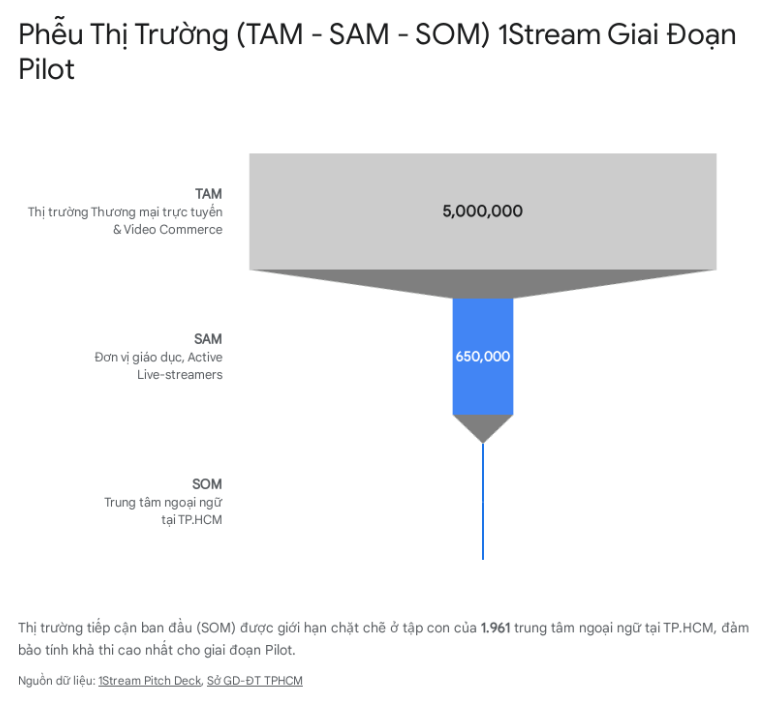
\includegraphics[width=0.85\linewidth]{imgs/PA3_pics/image1_v2.png}
    \caption{Mô hình phễu TAM -- SAM -- SOM cho 1Stream giai đoạn Pilot}
    \label{fig:tam-sam-som}
\end{figure}

\begin{WarningBox}[GIẢ ĐỊNH VỀ TỶ LỆ XUYÊN THẤU VÀ TẬP CON SOM]
Phân tích trên sử dụng con số 1.961 trung tâm\footnote{Nguồn: TPHCM: Khuyến khích mô hình câu lạc bộ của trung tâm ngoại ngữ, tin học (đã dẫn).} làm nền tảng SOM, đây là một điểm neo dữ liệu cứng đáng tin cậy. Tuy nhiên, lập luận cho rằng sẽ có \textbf{tối thiểu 15--20\%} trong tổng số các trung tâm này (tương đương khoảng 300 đến 400 trung tâm) sẽ thỏa mãn một cách hoàn hảo toàn bộ các bộ lọc nhận diện khắt khe (đội ngũ marketing chuẩn 3--5 người, chạy ads tích cực hàng ngày, có cấu trúc data khóa học chuẩn) hoàn toàn là một GIẢ ĐỊNH mang tính lạc quan. Đội ngũ Marketing của dự án không được phép tin tưởng tuyệt đối vào tỷ lệ này. Họ bị bắt buộc phải tiến hành thực thi các chiến dịch khai thác và cào dữ liệu kỹ thuật số (Data Scraping) một cách tinh vi, sử dụng các công cụ như Facebook Ads Library, để tiến hành kiểm chứng chéo và đo lường con số trung tâm thực tế đạt tiêu chuẩn trước khi quyết định ký duyệt giải ngân bất kỳ một khoản ngân sách quảng cáo lớn nào.
\end{WarningBox}

%% ================================================================
%% SECTION 5
%% ================================================================
\subsubsection{Nghệ thuật Tiếp cận Trinh sát số (Digital Reconnaissance) và Dẫn dắt Go-To-Market (GTM) qua Lăng kính Đánh giá Tiềm năng}

Phần phân tích này nhằm trả lời trực tiếp và sâu sát nhất cho bài toán cốt lõi: \textit{Làm thế nào để đội ngũ tiếp thị (Marketing) có thể nhận diện chính xác cái ICP cốt lõi đó giữa một thị trường bao la và hỗn loạn?} Chiến lược tiếp cận thị trường (GTM) trong giai đoạn Pilot của 1Stream không bao giờ được phép sa lầy vào tư duy mua các luồng lưu lượng truy cập giá rẻ hay chạy quảng cáo dàn trải trên diện rộng (Mass Marketing). Thay vào đó, chiến lược được định hình như một nghệ thuật ``săn lùng'' các tín hiệu số đặc thù (Digital Signals) và thực thi quy trình phân loại dữ liệu (Lead Qualification) cực đoan.

\paragraph{Cơ chế ``Săn'' ICP Cốt lõi trên không gian Digital (Digital Footprint Reconnaissance)}

Để phát hiện và nhận diện các trung tâm tiếng Anh hoặc tiếng Hàn hoàn hảo cho dự án, đội ngũ Marketing không thể áp dụng phương pháp gọi điện chào hàng lạnh (Cold Calling) một cách ngẫu nhiên từ danh bạ doanh nghiệp. Sự lãng phí thời gian vào các trung tâm không chạy quảng cáo số sẽ giết chết hiệu suất của bộ phận Sales. Thay vào đó, một quy trình nhận diện chủ động (Outbound Identification) dựa trên trí tình báo kỹ thuật số mã nguồn mở (OSINT) được thiết lập thông qua ba bước kỹ thuật sau:

Quy trình đầu tiên là thiết lập trạm quét tình báo thông qua Thư viện quảng cáo (Facebook Ads Library Recon). Chuyên viên tiếp thị của 1Stream sẽ sử dụng Facebook Ads Library, một công cụ minh bạch dữ liệu do Meta cung cấp\footnote{Nguồn: Facebook Ads là gì? Hướng dẫn chi tiết từ A -- Z -- CareerViet, truy cập ngày 16 tháng 7 năm 2026, \url{https://careerviet.vn/vi/talentcommunity/facebook-ads-la-gi-huong-dan-chi-tiet-tu-a-z.35A522A4.html}}, kết hợp với các bộ lọc từ khóa chuyên ngành được tối ưu hóa cao độ (ví dụ: ``Khóa học IELTS cam kết đầu ra'', ``Luyện thi TOPIK cấp tốc'', ``Ưu đãi học phí tiếng Anh tháng này'', ``Đăng ký test đầu vào miễn phí''). Khi quét hệ thống này, bất kỳ một Fanpage trung tâm nào duy trì việc chạy từ 5 chiến dịch quảng cáo mang tính chất chuyển đổi (Conversion Ads) trở lên cùng một lúc, đặc biệt nếu họ sử dụng các định dạng video ngắn dọc hoặc phát lại các đoạn cắt từ livestream (livestream replay), đều lập tức phát ra một tín hiệu số cực mạnh chứng minh họ ``đang chạy số'' quyết liệt. Phân tích tâm lý học kinh doanh cho thấy, các trung tâm này đang phải thiêu đốt một lượng ngân sách khổng lồ mỗi ngày và họ đang trong trạng thái khao khát đến tuyệt vọng việc tìm ra các phương pháp tối ưu hóa chỉ số CPL.\footnote{Nguồn: CHIẾN DỊCH QUẢNG CÁO KHÓA HỌC TIẾNG ANH TRÊN FACEBOOK VỚI NGÂN SÁCH 9.000.000Đ/THÁNG -- SPEAK NOW, truy cập ngày 16 tháng 7 năm 2026, \url{https://speaknow.vn/phu-kim-quy-chia-se-chien-dich-quang-cao-khoa-hoc-tieng-anh-tren-facebook/}} Sự xuất hiện của 1Stream lúc này chính là giải pháp dập tắt cơn đau tài chính đó.

Quy trình thứ hai là chiến dịch Giám sát Khung giờ vàng Livestream trên nền tảng TikTok (TikTok Live Monitoring). Đội ngũ sẽ triển khai các công cụ phân tích tự động hoặc phân công trực ban thủ công để rà quét các luồng phát sóng vào đúng khung giờ sinh tử từ 19h00 đến 22h30 mỗi tối.\footnote{Nguồn: GMV Max là gì? AI campaign đột phá của TikTok Shop 2026 | OneZ (đã dẫn).} Một tín hiệu nhận diện MQL (Marketing Qualified Lead) hoàn hảo nhất sẽ xuất hiện dưới hình thái sau: Khám phá ra một kênh TikTok của một trung tâm ngoại ngữ đang trong trạng thái phát sóng trực tiếp (LIVE), lượng người xem đồng thời (Concurrent Viewers -- CCV) duy trì ổn định nhưng không quá cao, dao động từ 30 đến 100 người. Tuy nhiên, tốc độ bình luận (comments per minute) từ khán giả diễn ra liên tục, nhưng người dẫn chương trình (Host) hoặc đội ngũ hỗ trợ phía sau lại có tốc độ phản hồi bằng văn bản quá chậm, liên tục đọc sót tên người dùng đang hỏi về thông tin khóa học. Khung cảnh hỗn loạn nhẹ này chính là biểu hiện vật lý rõ nét nhất của ``cường độ vấn đề'' (Pain Point) mà trung tâm đang gặp phải. Đây là cơ hội hoàn hảo để tác nhân AI Agent của 1Stream can thiệp, chứng minh khả năng phản hồi chính xác từng câu hỏi trong vòng vài giây mà không bao giờ biết mệt mỏi hay bỏ sót bất kỳ một khách hàng tiềm năng nào.

Quy trình thứ ba, mang tính quyết định trước khi thực hiện bước tiếp cận, là quá trình Đánh giá mức độ Chuẩn hóa Dữ liệu nội bộ (Data Readiness Check). Ngay sau khi phát hiện các tín hiệu mạnh từ hai bước trên, chuyên viên Marketing không được phép liên hệ ngay. Họ phải thực hiện một cuộc kiểm tra tĩnh bằng cách truy cập trực tiếp vào giao diện website chính thức hoặc cấu trúc trang đích (Landing Page) của trung tâm mục tiêu đó. Đích đến của cuộc kiểm tra là hệ thống phân cấp thông tin. Nếu trung tâm đó xây dựng một hệ thống Menu rõ ràng, sở hữu các trang con minh bạch về Báo giá (Pricing), Lịch khai giảng (Schedules) được cập nhật thường xuyên, và Hệ thống Câu hỏi Thường gặp (FAQ) đầy đủ -- thì luồng dữ liệu (Lead) này chính thức được đóng dấu ``Đủ điều kiện Data hoàn hảo''. Nó lập tức được đẩy thẳng xuống bước đánh giá sâu hơn, bởi hệ thống của họ đã sẵn sàng để trở thành cơ sở tri thức (Knowledge Base) huấn luyện cho AI của 1Stream mà không cần phải chỉnh sửa gì thêm.

\paragraph{Khái niệm lại Khung Phân loại Lead: Sự khác biệt giữa MQL và SQL trong Đặc thù ngành EdTech}

Để thiết lập một bức tường lửa bảo vệ thời gian của đội ngũ Sales, ngăn chặn tuyệt đối tình trạng gọi điện thoại nhầm đối tượng, quy trình chuyển đổi trạng thái vòng đời từ Marketing Qualified Lead (MQL) sang Sales Qualified Lead (SQL) phải được định nghĩa lại một cách căn bản cho phù hợp với những biến số đặc thù của ngành EdTech kết hợp SaaS. Tham chiếu các dữ liệu toàn cầu cho thấy, tỷ lệ chuyển đổi trung bình từ MQL sang SQL trong các doanh nghiệp cung cấp dịch vụ phần mềm B2B (B2B SaaS) thường duy trì ở mức khá cao, dao động ổn định trong khoảng từ 32\% đến 40\%.\footnote{Nguồn: B2B SaaS Conversion Rate Benchmarks 2026 by Funnel Stage, truy cập ngày 16 tháng 7 năm 2026, \url{https://konabayev.com/blog/b2b-saas-conversion-benchmarks-2026/}} Tỷ lệ này phản ánh một thị trường doanh nghiệp có tư duy hệ thống và chu kỳ mua sắm phần mềm rõ ràng. Tuy nhiên, khi áp dụng cùng một mô hình vào mảng giáo dục (EdTech) nói chung và các trung tâm ngoại ngữ nói riêng, tỷ lệ chuyển đổi này sụp đổ và rớt xuống một mức rất thấp, chỉ quanh quẩn ở ngưỡng 5\% đến 10\%.\footnote{Nguồn: How To: Turn MQLs into SQLs | EM360Tech, truy cập ngày 16 tháng 7 năm 2026, \url{https://em360tech.com/blog/mql-to-sql-guide}} Nguyên nhân của sự sụt giảm này xuất phát từ chu kỳ ra quyết định mua sắm của các giám đốc giáo dục thường bị kéo dài, sự dè dặt với các công nghệ AI mới, và tính chất phân mảnh cao của các cơ sở đào tạo quy mô nhỏ.

Đối mặt với thực trạng tỷ lệ chuyển đổi khắc nghiệt này, khung đánh giá năng lực tiềm năng của 1Stream được thiết lập vô cùng hà khắc và chia làm hai ranh giới phân định rõ ràng.

Ranh giới đầu tiên là việc định danh \textbf{MQL (Marketing Qualified Lead) -- Lead Đủ điều kiện Tiếp thị}. Để được công nhận là một MQL, hồ sơ đó phải là thông tin của một trung tâm ngoại ngữ đang hoạt động tại khu vực TP.HCM (tức là đã vượt qua thành công màng lọc vị trí địa lý của thị trường SOM). Hồ sơ này có thể do trung tâm tự nguyện để lại thông tin liên hệ, hoặc là kết quả do đội ngũ Marketing của 1Stream ``săn lùng'' thành công từ các chiến dịch trinh sát trên Facebook hay TikTok. Hơn thế nữa, MQL này bắt buộc phải thể hiện các hành vi số (Digital behavior) rõ nét, chẳng hạn như: có dữ liệu truy cập vào trang chủ của nền tảng 1Stream, nhấp chuột xem qua các trang giới thiệu tính năng lõi như ``AI Auto-Reply'', hoặc chủ động điền email công ty vào các biểu mẫu nhận bản tin. MQL là tín hiệu cho thấy sự quan tâm ban đầu, nhưng tuyệt đối chưa đủ độ chín để chuyển giao cho bộ phận bán hàng.

Ranh giới thứ hai, và cũng là giới hạn sinh tử, là việc thăng cấp lên \textbf{SQL (Sales Qualified Lead) -- Lead Đủ điều kiện Bán hàng}. Một MQL đang nằm trong hệ thống dữ liệu chỉ được phép thăng cấp và trao danh hiệu SQL khi và chỉ khi bộ phận Marketing đã thực hiện thành công bước xác minh chéo. Bước xác minh này thường được tiến hành qua một cuộc gọi sơ bộ đánh giá nhu cầu (Discovery call) hoặc một biểu mẫu khảo sát thông minh, nhằm đảm bảo MQL đó đáp ứng đồng thời ba tiêu chí bất khả kháng: Thứ nhất, họ xác nhận đội ngũ Marketing hoặc trực Live của họ hiện có quy mô chính xác từ 3 đến 5 nhân sự; Thứ hai, họ sở hữu và sẵn sàng cung cấp các tài liệu giáo trình và bảng giá dưới dạng dữ liệu tĩnh; Thứ ba, nhân sự mà 1Stream đang trao đổi phải là người có thực quyền ra quyết định cuối cùng (Decision Maker), hoặc chí ít là người bảo trợ dự án (Champion) có khả năng gây ảnh hưởng trực tiếp đến ngân sách mua sắm công cụ phần mềm của trung tâm. Bất kỳ sự thiếu hụt nào trong ba tiêu chí này đều khiến MQL bị giáng cấp. Chỉ những hồ sơ vượt qua khe cửa hẹp này, trở thành SQL thực thụ, mới được đặc cách chuyển giao cho đội ngũ Chuyên viên Phát triển Tài khoản cấp cao (Account Executive) để tiến hành dàn xếp các buổi trình diễn (demo) sản phẩm thực tế.

\begin{figure}[H]
    \centering
    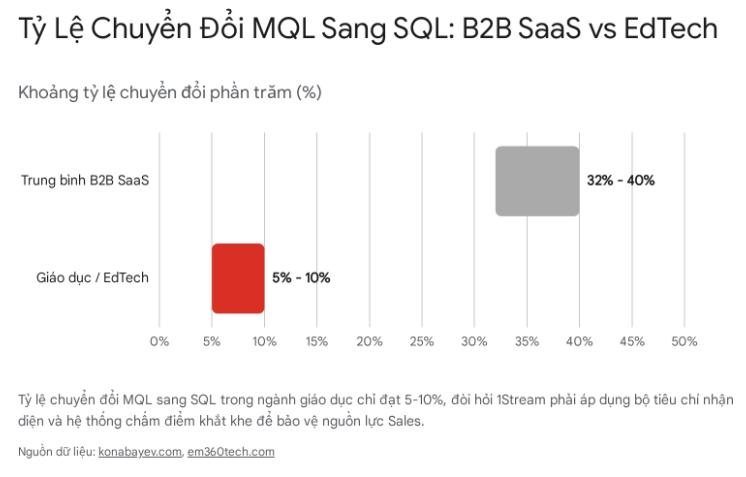
\includegraphics[width=0.85\linewidth]{imgs/PA3_pics/image2_v2.png}
    \caption{So sánh tỷ lệ chuyển đổi MQL-to-SQL giữa B2B SaaS và EdTech}
    \label{fig:mql-sql-comparison}
\end{figure}

%% ================================================================
%% SECTION 6
%% ================================================================
\subsubsection{Kiến trúc Hệ thống Chấm điểm Định lượng ICP (Lead Scoring Matrix) Dành cho Giai đoạn Pilot}

Quá trình chuyển hóa các đặc tính phân tích định tính về sự phù hợp của khách hàng từ các báo cáo phát triển sản phẩm (chương PA2) thành một công cụ định lượng sắc bén, có thể hoạt động độc lập trên hệ thống phần mềm thực chiến của đội ngũ Marketing, là bước đi bắt buộc. Để hiện thực hóa điều này, chúng tôi đã kiến tạo một Hệ thống chấm điểm đánh giá tiềm năng khách hàng (Lead Scoring Matrix) hoạt động dựa trên cơ chế trọng số tối đa là 100 điểm. Mọi tương tác, đặc điểm tổ chức và hành vi của một Khách hàng tiềm năng (Lead) đều sẽ được hệ thống theo dõi và cộng dồn điểm số. Khái niệm phân loại sẽ được tự động hóa hoàn toàn: chỉ những hồ sơ tích lũy vượt qua được ranh giới điểm quy định (Threshold) mới được quyền kích hoạt quy trình báo động chuyển đổi thành SQL.

\paragraph{Cấu trúc Thuật toán Thang điểm 100 và Bộ Tiêu chí Đánh giá}

Ma trận chấm điểm này không phân bổ điểm số đồng đều mà sử dụng nguyên tắc trọng số, trong đó những yếu tố quyết định khả năng áp dụng công nghệ AI ngay lập tức sẽ nắm giữ số điểm cao nhất.

\begin{table}[H]
    \centering
    \footnotesize
    \setlength{\tabcolsep}{3pt}
    \renewcommand{\arraystretch}{1.25}
    \caption{Ma trận chấm điểm đánh giá tiềm năng khách hàng (Lead Scoring Matrix) -- Thang 100 điểm}
    \label{tab:lead-scoring}
    \rowcolors{2}{paperBg}{white}
    \begin{tabularx}{\linewidth}{@{}L{0.14\linewidth}YL{0.08\linewidth}Y@{}}
        \toprule
        \rowcolor{softBlue}
        \textbf{Tiêu chí Đánh giá Cốt lõi (Core Criteria)} &
        \textbf{Diễn giải Cơ chế \& Quy trình Marketing thu thập tín hiệu} &
        \textbf{Phân bổ Trọng số} &
        \textbf{Khung Điểm Phạt (Negative / Penalty Logic)} \\ \midrule

        %% --- Row 1 ---
        \textbf{Cường độ vấn đề (Pain Point Intensity)} &

        Đo lường mức độ khủng hoảng trong vận hành hiện tại, đặc biệt là tình trạng quá tải bình luận và sự gia tăng mất kiểm soát của chi phí CPL.

        \textbf{Cơ chế thu thập:} Các kỹ thuật viên Marketing phát hiện trung tâm có tỷ lệ rớt bình luận cao trên livestream TikTok, hoặc đang đổ tiền chạy quảng cáo liên tục trên FB Ads Library nhưng hệ thống Landing Page lại hoàn toàn vắng bóng các công cụ phản hồi tự động (chatbots) ban đầu. &

        \textbf{20 điểm} &

        $-20$ điểm (Áp dụng ngay lập tức nếu dữ liệu cho thấy livestream của trung tâm có lượng người xem bằng 0 hoặc trung tâm không hề triển khai bất kỳ chiến dịch quảng cáo trả phí nào trong vòng 30 ngày qua). \\ \midrule

        %% --- Row 2 ---
        \textbf{Sự tương thích về quy mô nguồn lực (Marketing Team Size)} &

        Đánh giá tính lý tưởng của cấu trúc nhân sự, hướng tới điểm ngọt từ 3 đến 5 người.

        \textbf{Cơ chế thu thập:} Chuyên viên thực hiện các nghiệp vụ tra cứu thông tin tình báo doanh nghiệp thông qua mạng lưới LinkedIn, hoặc theo dõi các cổng thông tin việc làm (như Ybox, CareerViet) để xem trung tâm có đang trong tình trạng đăng tin tuyển dụng khẩn cấp các vị trí chuyên viên Facebook Ads hay Livestreamer ca tối hay không.\footnote{Nguồn: [Online] Trung Tâm Tiếng Anh IGEMS Tuyển Dụng Thực Tập Sinh Dạy Tiếng Anh -- Livestream Full-time 2025 -- YBOX (đã dẫn).} &

        \textbf{15 điểm} &

        0 điểm (Hệ thống không cộng điểm nếu quy mô đội ngũ quá manh mún dưới 2 người, hoặc cấu trúc đã phình to quá phức tạp trên 10 người). \\ \midrule

        %% --- Row 3 ---
        \textbf{Mật độ và Tần suất sử dụng (Usage Frequency)} &

        Xác nhận thói quen duy trì các phiên phát sóng trực tiếp một cách đều đặn vào các khung giờ vàng buổi tối (19h00--22h30). Đi kèm với đó là nhu cầu hiển nhiên về việc sản xuất các đoạn video ngắn hàng ngày để duy trì tương tác. &

        \textbf{15 điểm} &

        $-10$ điểm (Trừ điểm mạnh nếu hồ sơ chỉ ra rằng trung tâm chỉ duy trì lịch livestream mang tính sự kiện, ví dụ 1 tháng chỉ tổ chức 1 lần). \\ \midrule

        %% --- Row 4 ---
        \textbf{Mức độ chuẩn hóa của Khối Dữ liệu tĩnh (Data Standardization)} &

        Kiểm định khả năng cung cấp nền tảng tri thức cho AI, thông qua việc có sẵn các bảng giá cố định và lộ trình học mang tính chất tĩnh.

        \textbf{Cơ chế thu thập:} Bot thu thập hoặc chuyên viên truy cập trực tiếp website của trung tâm, nếu hệ thống điều hướng (menu) có chứa các thư mục công khai như ``Học phí'', ``Lịch khai giảng'', hồ sơ lập tức đạt điểm tối đa ở hạng mục này. &

        \textbf{15 điểm} &

        $-20$ điểm (Phạt nặng nếu hệ thống phát hiện chính sách tiếp thị của trung tâm là ``Inbox để nhận báo giá bí mật'', khiến AI không có cơ sở dữ liệu để vận hành). \\ \midrule

        %% --- Row 5 ---
        \textbf{Năng lực chi trả và Dòng tiền tiếp thị (Willingness to Pay)} &

        Phân tích tiềm lực tài chính dựa trên bằng chứng về việc có phân bổ ngân sách Marketing rõ ràng. Các ước tính vĩ mô chỉ ra rằng những trung tâm duy trì chạy ads liên tục sẽ phải gánh CPL trung bình 24.584 VNĐ và sở hữu một ngân sách duy trì dài hạn.\footnote{Nguồn: Chạy quảng cáo Facebook bao nhiêu tiền cập nhật mới nhất | On Digitals -- Ondigitals (đã dẫn).} Sự sẵn sàng đầu tư này chứng minh họ đủ sức chi trả cho các gói thuê bao của một công cụ SaaS. &

        \textbf{15 điểm} &

        0 điểm (Áp dụng cho các mô hình dự án sinh viên khởi nghiệp phi lợi nhuận, hoặc các trung tâm hoạt động cộng đồng miễn phí không có nhu cầu tối ưu hóa lợi nhuận). \\ \midrule

        %% --- Row 6 ---
        \textbf{Khả năng Tích hợp Độc lập (Tech Fit / No Complex API)} &

        Đánh giá mức độ sẵn lòng chấp nhận sử dụng giao diện bảng điều khiển (dashboard) độc lập của 1Stream, thay vì đưa ra các yêu sách đòi hỏi đội ngũ kỹ thuật phải viết mã kết nối API cắm sâu vào hệ thống ERP cồng kềnh của tập đoàn. &

        \textbf{10 điểm} &

        $-50$ điểm (Đây là án phạt mang tính chất vô hiệu hóa hồ sơ, áp dụng khi khách hàng khăng khăng đòi hỏi các giao thức kết nối API phức tạp ngay trong tháng chạy Pilot). \\ \midrule

        %% --- Row 7 ---
        \textbf{Rào cản Tính hợp pháp (Pháp lý sinh trắc học)} &

        Xác nhận tuyệt đối quyền sở hữu bản quyền hợp pháp đối với hình ảnh và đặc điểm giọng nói của nhân sự sẽ được sử dụng làm nguồn để huấn luyện AI. (Yếu tố này thường được đánh giá trực tiếp qua khảo sát đầu vào trong cuộc gọi Discovery Call). &

        \textbf{10 điểm} &

        \textbf{LOẠI TRỰC TIẾP} (Nếu khách hàng bộc lộ sự mập mờ hoặc không chứng minh được tính pháp lý, toàn bộ hồ sơ lập tức bị đóng băng bất kể tổng điểm các phần khác cao đến đâu). \\ \midrule

        %% --- Row TOTAL ---
        \textbf{TỔNG KIỂM SOÁT TỐI ĐA} & & \textbf{100 điểm} & \\

        \bottomrule
    \end{tabularx}
    \rowcolors{2}{}{}
\end{table}

\paragraph{Thuật toán Ngưỡng Phân loại và Quy trình Chuyển giao (Threshold Handoff Rules)}

Được vận hành trên nền tảng của cấu trúc tính điểm chi tiết ở trên, luồng làm việc tự động (Automated Workflow) giữa bộ phận Marketing thu thập dữ liệu và bộ phận Sales chốt hợp đồng sẽ được vận hành một cách trơn tru, lạnh lùng và không có chỗ cho cảm tính cá nhân, cụ thể như sau:

Cấp độ đầu tiên, áp dụng cho dải điểm \textbf{Từ 0 đến 45 Điểm}: Những hồ sơ rơi vào vùng trũng này sẽ ngay lập tức được hệ thống gán nhãn là ``Cold Lead'' (Lead lạnh) hoặc ``Nurture'' (Cần nuôi dưỡng). Về cơ bản, đây chính là nhóm khách hàng thuộc Phân khúc liền kề (Adjacent Segment) hoặc nhóm Chưa ưu tiên do thiếu hụt ngân sách hoặc chưa sẵn sàng về mặt dữ liệu. Đội ngũ Marketing sẽ tự động đưa các liên hệ này vào một phễu gửi Email tự động dài hạn nhằm mục đích giáo dục thị trường, cập nhật các tính năng mới hoặc gửi các báo cáo ngành. Tại dải điểm này, hoàn toàn không có sự tham gia của bất kỳ nhân sự Sales nào để tránh lãng phí thời gian.

Cấp độ thứ hai, áp dụng cho dải điểm \textbf{Từ 46 đến 74 Điểm}: Các hồ sơ vượt qua ngưỡng 45 điểm sẽ chính thức được thăng cấp vào nhóm MQL. Trạng thái này kích hoạt một nhiệm vụ cho đội ngũ phát triển kinh doanh vòng ngoài (như Telesales hoặc Sales Development Representative -- SDR). Họ sẽ có nhiệm vụ thực hiện một cuộc gọi điện thoại sơ bộ (Discovery Call), được khống chế nghiêm ngặt không quá 5 phút. Mục tiêu duy nhất của cuộc gọi này là để xác thực các giả định mà hệ thống chấm điểm đã gán, đặc biệt xoáy sâu vào việc xác minh lại Cường độ vấn đề đang gặp phải và Mức độ chuẩn hóa của dữ liệu nội bộ.

Cấp độ thứ ba, cấp độ tối cao, áp dụng cho dải điểm \textbf{Từ 75 đến 100 Điểm}: Bất kỳ hồ sơ nào lọt vào dải điểm này sẽ chính thức rũ bỏ mọi sự nghi ngờ để trở thành một \textbf{Core ICP (SQL)} hoàn hảo. Lúc này, hệ thống sẽ tự động kích hoạt lệnh chuyển thẳng Lead đó vào hệ thống Quản trị Quan hệ Khách hàng (CRM) nội bộ, đồng thời phân công trực tiếp cho các Chuyên viên Phát triển Tài khoản cấp cao (Account Executive). Đây là những bức chân dung của một trung tâm ngoại ngữ lý tưởng: họ có một đội ngũ 4 người đang kiệt sức, họ đang thiêu đốt hàng chục triệu đồng để chạy quảng cáo Facebook mỗi tháng\footnote{Nguồn: Facebook Ads Cho Giáo Dục: Checklist Hoàn Chỉnh (2026) -- NgoiSaoMedia (đã dẫn).}, họ liên tục tổ chức livestream bất chấp lượng người xem đôi khi khiêm tốn, họ có bảng giá công khai minh bạch rõ như ban ngày, và quan trọng nhất, họ đang bị ``ngộp thở'' trong vòng xoáy của việc phải phản hồi hàng trăm bình luận một cách thủ công. Nhiệm vụ của đội ngũ Sales lúc này không còn là ``thuyết phục'' họ sử dụng phần mềm, mà là hành động như những vị cứu tinh: Sales sẽ ưu tiên tối đa việc thiết lập ngay các buổi trình diễn tính năng (Demo) trực tiếp -- có thể qua các nền tảng trực tuyến hoặc ưu tiên gặp mặt trực tiếp (Offline) tại trụ sở trung tâm ở TP.HCM -- và ngay lập tức đưa ra đề xuất chốt hợp đồng đối với Gói dịch vụ 30 giờ/kênh của nền tảng 1Stream.

\begin{WarningBox}[GIẢ ĐỊNH VỀ TÍNH CHÍNH XÁC CỦA HỆ THỐNG CHẤM ĐIỂM TỰ ĐỘNG BẰNG OSINT]
Cơ chế vận hành của quy trình đánh giá các tiêu chí mang tính định lượng như ``Tần suất sử dụng'' và đặc biệt là ``Mức độ chuẩn hóa Data'' hiện tại đang được xây dựng trên một giả định cốt lõi: Các kỹ thuật viên Marketing của dự án, hoặc các hệ thống thu thập dữ liệu tự động, có khả năng trích xuất đầy đủ các thông tin công khai (Open-Source Intelligence -- OSINT) trên môi trường Internet mà không tốn quá nhiều thời gian quét thủ công. Tuy nhiên, rủi ro sai lệch xuất hiện nếu thiết kế Website của khách hàng cố tình ẩn giấu cấu trúc dữ liệu đào tạo (bảng giá, lịch học) đằng sau một bức tường biểu mẫu đăng ký (gated content) buộc người dùng phải điền thông tin mới được xem. Trong trường hợp này, điểm số đánh giá sẽ bị đánh tụt một cách oan uổng. Để giải quyết rủi ro này, quy trình vận hành bắt buộc phải kết hợp sử dụng các biểu mẫu thu thập thông tin hấp dẫn (Lead Magnet Form) chứa các bảng câu hỏi yêu cầu chính các chủ trung tâm phải tự đánh giá hiện trạng của họ (Self-assess), từ đó lấy dữ liệu chủ quan này để đối chiếu chéo với dữ liệu khách quan thu thập được, đảm bảo tính chính xác tuyệt đối trước khi ra quyết định phân loại Lead.
\end{WarningBox}

%% ================================================================
%% SECTION 7
%% ================================================================
\subsubsection{Khuyến nghị Triển khai Chiến lược Tối ưu hóa Hành trình Khách hàng}

Việc đưa ra quyết định chiến lược đóng gói toàn bộ giá trị công nghệ phức tạp của 1Stream thành một Gói sản phẩm tiêu chuẩn 30 giờ/kênh, đồng thời nhắm mục tiêu một cách cực đoan vào một ngách thị trường cụ thể là các trung tâm ngoại ngữ có trụ sở tại TP.HCM, là một nước đi chiến lược cực kỳ sắc bén (Laser-focused strategy). Thay vì rơi vào cái bẫy ảo tưởng của việc cố gắng bán một giải pháp chung chung cho hàng triệu người bán hàng trên mạng xã hội -- một nỗ lực thường dẫn đến sự pha loãng định vị thương hiệu và cạn kiệt dòng tiền -- việc dồn toàn lực tập trung vào các trung tâm đào tạo IELTS hay TOEIC có quy mô vận hành nhỏ giúp sản phẩm kiểm chứng (validate) được cốt lõi công nghệ AI của mình một cách an toàn, nhanh chóng và có khả năng thu hồi vốn, đồng thời vẫn bảo vệ được nguồn lực giới hạn của đội ngũ R\&D.

Để các hoạt động tiếp thị (Marketing) thực sự nhận diện được chính xác cái ICP cốt lõi đang lẩn khuất trên thị trường một cách hiệu quả nhất, ba nhóm hành động chiến thuật mang tính mệnh lệnh dưới đây bắt buộc phải được triển khai trên thực địa ngay lập tức, không có bất kỳ sự nhân nhượng nào:

Hành động thứ nhất đòi hỏi một sự thay đổi tư duy triệt để trong việc phân bổ ngân sách: \textbf{Chấm dứt vô điều kiện mọi chiến dịch quảng cáo diện rộng mang tính chất ``Mass Ads''.} Đội ngũ tiếp thị phải ngay lập tức ngừng việc đổ tiền vào các chiến dịch quảng cáo hiển thị rộng rãi, nhắm mục tiêu vào các từ khóa mơ hồ mang tính chất khái quát cao như ``Giải pháp livestream toàn diện'' hay ``Phần mềm tăng đơn hàng''. Toàn bộ ngân sách giải phóng được từ đây phải được chuyển hướng và tái cấu trúc hoàn toàn sang các mô hình tiếp thị có độ chính xác cao hơn, cụ thể là Tiếp thị thu hút (Inbound Marketing) và đặc biệt là mô hình Tiếp thị Dựa trên Tài khoản (Account-Based Marketing -- ABM). Mục tiêu của các chiến dịch này không phải là đám đông, mà được thiết kế như những mũi tên bắn thẳng tới các cá nhân nắm giữ các chức danh cụ thể như ``Giám đốc trung tâm đào tạo'', ``Founder học viện ngoại ngữ'', hay ``Trưởng phòng Marketing Giáo dục'', và phải giới hạn khu vực phân phối quảng cáo bằng hàng rào địa lý (geo-fencing) nằm gọn trong ranh giới TP.HCM.

Hành động thứ hai định hình lại thông điệp truyền thông: \textbf{Sử dụng chính ``Nỗi đau CPL'' của khách hàng làm mồi nhử chết người (Lead Magnet).} Phân tích của các chuyên gia trong ngành đã chỉ ra một sự thật phũ phàng: chi phí CPL cho ngành giáo dục, dù trên lý thuyết các báo cáo thường được tô vẽ ở mức thấp (quanh ngưỡng 24.000 VNĐ)\footnote{Nguồn: Chạy quảng cáo Facebook bao nhiêu tiền cập nhật mới nhất | On Digitals -- Ondigitals (đã dẫn).}, nhưng trong môi trường thực chiến chạy Facebook Ads với sự cạnh tranh đẫm máu, mức chi phí này hoàn toàn có thể vọt lên tới nửa triệu đồng (500.000 VNĐ) cho một Lead.\footnote{Nguồn: Facebook Ads Cho Giáo Dục: Checklist Hoàn Chỉnh (2026) -- NgoiSaoMedia (đã dẫn).} Nguyên nhân chủ đạo của sự lãng phí này là tỷ lệ thoát trang (bounce rate) và sự rời bỏ của khách hàng do tốc độ phản hồi tin nhắn của trung tâm quá chậm chạp. Thông điệp Marketing của 1Stream không được phép nói về các thuật ngữ kỹ thuật khô khan của AI. Thông điệp phải đâm thẳng vào nỗi sợ hãi tài chính của chủ doanh nghiệp: \textit{``AI Agent của nền tảng chúng tôi sẽ đứng gác và giữ chân từng học viên của bạn lúc 22h00 đêm, ngay cả khi toàn bộ đội ngũ tư vấn của bạn đã đi ngủ. Chúng tôi cam kết chặn đứng sự rò rỉ ngân sách và ép CPL của bạn giảm xuống 3 lần''}. Bằng chứng thực nghiệm luôn cho thấy, các thông điệp đánh trực diện vào hiệu quả tài chính và nỗi sợ mất tiền luôn mang lại tỷ lệ chuyển đổi từ dữ liệu thô sang SQL cao nhất trong mọi chiến dịch tiếp thị B2B.

Hành động thứ ba, và là hành động khó khăn nhất về mặt tâm lý đối với đội ngũ bán hàng: \textbf{Thiết lập kỷ luật Tôn trọng Tiêu chí Loại trừ một cách tuyệt đối (Zero Tolerance Policy).} Ban giám đốc dự án không được phép thỏa hiệp, không được phép bẻ cong nguyên tắc để tiếp nhận bất kỳ một khách hàng nào không chứng minh được họ có hệ thống dữ liệu tĩnh rõ ràng, hoặc những khách hàng khăng khăng đưa ra yêu sách tích hợp API rườm rà. Phải thấm nhuần tư tưởng rằng, mục tiêu tối thượng của giai đoạn Pilot không phải là chạy theo doanh thu tối đa bằng mọi giá, mà là chứng minh được tính khả thi của năng lực kỹ thuật cốt lõi và kiến tạo nên những Câu chuyện thành công (Case Study) mang tính đại diện hoàn hảo. Việc cố gắng nuông chiều và chốt một hợp đồng từ một Enterprise Lead (Khách hàng doanh nghiệp lớn) ngay trong giai đoạn Pilot, với hy vọng vào một khoản doanh thu lớn, thực chất là một liều thuốc độc. Nó sẽ bào mòn đến kiệt quệ nguồn lực vốn đã ít ỏi của đội ngũ kỹ thuật, làm trễ nải tiến độ hoàn thiện phiên bản sản phẩm thương mại (MVP), và cuối cùng có thể đánh sập toàn bộ cấu trúc kiến trúc phần mềm vì phải chắp vá để phục vụ một hệ thống quá tầm kiểm soát.

Chiến lược phân khúc khách hàng chuyên sâu và kế hoạch tiếp cận thị trường (GTM) này không phải là những ý tưởng lý thuyết suông. Nó được xây dựng và đúc kết trên sự thấu hiểu sâu sắc không chỉ về kiến trúc sản phẩm của 1Stream, mà quan trọng hơn là sự thấu hiểu về bản chất tàn khốc và sự khắc nghiệt trong hệ sinh thái cạnh tranh của ngành Giáo dục -- Ngoại ngữ hiện đại. Việc tuân thủ một cách tuyệt đối và kỷ luật đối với khung phân khúc thị trường đã được thiết lập này không chỉ là một khuyến nghị, mà sẽ là yếu tố duy nhất quyết định sinh mệnh và quỹ đạo thành công của dự án 1Stream trong giai đoạn thương mại hóa đầu tiên.

%% ================================================================
%% WORKS CITED / DANH MỤC NGUỒN THAM KHẢO
%% (Tất cả các nguồn đã được chuyển thành \footnote trong bản văn)
%% ================================================================
% [1]  Giáo dục trực tuyến edtech, elearning, đào tạo trực tuyến. đào tạo Online, accessed July 16, 2026, https://www.nguyentrihien.com/
% [2]  Báo cáo thị trường EdTech & eLearning Vietnam 2026 | PDF -- Slideshare, accessed July 16, 2026, https://www.slideshare.net/slideshow/bao-cao-th-tr-ng-edtech-elearning-vietnam-2026/286243550
% [3]  TPHCM: Khuyến khích mô hình câu lạc bộ của trung tâm ngoại ngữ, tin học, accessed July 16, 2026, https://gdthuongxuyen.hcm.edu.vn/tin-hoat-dong/tphcm-khuyen-khich-mo-hinh-cau-lac-bo-cua-trung-tam-ngoai-ngu-tin-hoc/ctmb/42180/82845
% [4]  TPHCM có 1.961 trung tâm ngoại ngữ, tin học, nhiều nơi quảng cáo sai sự thật, accessed July 16, 2026, https://laodong.vn/giao-duc/tphcm-co-1961-trung-tam-ngoai-ngu-tin-hoc-nhieu-noi-quang-cao-sai-su-that-1580712.ldo
% [5]  Trung tâm ngoại ngữ Hoàng Việt 6 năm liền nhận Giấy khen từ Sở GD&ĐT TP.HCM, accessed July 16, 2026, https://tuoitre.vn/khoahocphothong/trung-tam-ngoai-ngu-hoang-viet-6-nam-lien-nhan-giay-khen-tu-so-gd-dt-tp-hcm-261421.html
% [6]  Gần 2.000 trung tâm ngoại ngữ, tin học được cấp phép: Một số nơi quảng cáo sai sự thật, accessed July 16, 2026, https://tuoitre.vn/plo/gan-2000-trung-tam-ngoai-ngu-tin-hoc-duoc-cap-phep-mot-so-noi-quang-cao-sai-su-that-post872241.html
% [7]  Chạy quảng cáo Facebook bao nhiêu tiền cập nhật mới nhất | On Digitals -- Ondigitals, accessed July 16, 2026, https://ondigitals.com/vi/chay-quang-cao-facebook-bao-nhieu-tien/
% [8]  Tất tần tật về phí quảng cáo Facebook bạn nên biết -- BurgerPrints, accessed July 16, 2026, https://burgerprints.com/vi/phi-quang-cao-facebook/
% [9]  Facebook Ads Cho Giáo Dục: Checklist Hoàn Chỉnh (2026) -- NgoiSaoMedia, accessed July 16, 2026, https://ngoisaomedia.net/bai-viet/facebook-ads-cho-giao-duc-checklist-hoan-chinh-2026-1780978680408-9hta1/
% [10] Hàng nghìn phụ huynh yêu cầu hoàn trả học phí, TP. HCM dự kiến đình chỉ các trung tâm Apax Leaders -- VietnamFinance, accessed July 16, 2026, https://vietnamfinance.vn/hang-nghin-phu-huynh-yeu-cau-hoan-tra-hoc-phi-tp-hcm-du-kien-dinh-chi-cac-trung-tam-apax-leaders-d94889.html
% [11] TP HCM: Giải thể 20 trung tâm Anh ngữ Apax Leaders, accessed July 16, 2026, https://giaoducthudo.giaoducthoidai.vn/tp-hcm-giai-the-20-trung-tam-anh-ngu-apax-leaders-139178.html
% [12] [CSH2026][1Stream][FINAL PITCH DECK].pdf
% [13] GMV Max là gì? AI campaign đột phá của TikTok Shop 2026 | OneZ, accessed July 16, 2026, https://onezdigital.vn/blog/gmv-max-tiktok-shop-la-gi-2026
% [14] [Online] Trung Tâm Tiếng Anh IGEMS Tuyển Dụng Thực Tập Sinh Dạy Tiếng Anh -- Livestream Full-time 2025 -- YBOX, accessed July 16, 2026, https://ybox.vn/tuyen-dung/online-trung-tam-tieng-anh-igems-tuyen-dung-thuc-tap-sinh-day-tieng-anh-full-time-2025-67dd13aff49350455812bb8e
% [15] Học Tiếng Hàn Giao Tiếp Hiệu Quả -- Trung Tâm Ngoại Ngữ LingGo, accessed July 16, 2026, https://linggo.edu.vn/trung-tam-tieng-han-linggo-hoc-tieng-han-giao-tiep-hieu-qua/
% [16] Facebook Ads là gì? Hướng dẫn chi tiết từ A -- Z -- CareerViet, accessed July 16, 2026, https://careerviet.vn/vi/talentcommunity/facebook-ads-la-gi-huong-dan-chi-tiet-tu-a-z.35A522A4.html
% [17] 5 Bước Để Chạy Quảng Cáo Facebook Ads Cho Trung Tâm Ngoại Ngữ, accessed July 16, 2026, https://vietnamteachingjobs.com/blog/5-buoc-de-chay-facebook-ads-cho-trung-tam-ngoai-ngu/
% [18] CHIẾN DỊCH QUẢNG CÁO KHÓA HỌC TIẾNG ANH TRÊN FACEBOOK VỚI NGÂN SÁCH 9.000.000Đ/THÁNG -- SPEAK NOW, accessed July 16, 2026, https://speaknow.vn/phu-kim-quy-chia-se-chien-dich-quang-cao-khoa-hoc-tieng-anh-tren-facebook/
% [19] CPL là gì? Cách tính CPL (Cost per lead) & tối ưu quảng cáo CPL -- MISA AMIS, accessed July 16, 2026, https://amis.misa.vn/59497/cpl-la-gi/
% [20] B2B SaaS Conversion Rate Benchmarks 2026 by Funnel Stage, accessed July 16, 2026, https://konabayev.com/blog/b2b-saas-conversion-benchmarks-2026/
% [21] How To: Turn MQLs into SQLs | EM360Tech, accessed July 16, 2026, https://em360tech.com/blog/mql-to-sql-guide
% [22] Lead là gì? Các bước tạo lead dễ áp dụng cho người mới bắt đầu -- Vieclam24h, accessed July 16, 2026, https://vieclam24h.vn/nghe-nghiep/tram-sac-ky-nang/lead-la-gi


% --- PA3-01 | Trần Minh Quang ---
% ============================================================
% PHẦN 3.4 — CHÂN DUNG KHÁCH HÀNG ĐIỂN HÌNH
% ------------------------------------------------------------
% Thuộc: PA3-01
% Người phụ trách chính: Trần Minh Quang – Marketing Lead
% Phối hợp: Nguyễn Anh Thư
%
% CÂU HỎI CẦN TRẢ LỜI:
%   - Ai là người duyệt ngân sách?
%   - Ai là người sử dụng trực tiếp sản phẩm?
%   - Ai cung cấp dữ liệu khóa học cho hệ thống?
%   - Khách hàng cần có bao nhiêu nhân sự marketing, livestream và tư vấn?
%   - Nội dung nào thường xuyên bị lặp lại: học phí, lịch học, đầu vào, ưu đãi, học thử hay chính sách?
%
% OUTPUT BẮT BUỘC:
%   1. Chân dung người MUA HÀNG (Buying Persona):
%      - Ví dụ: Chủ trung tâm hoặc quản lý chi nhánh
%      - Mục tiêu kinh doanh
%      - Vấn đề
%      - Rào cản
%      - Tiêu chí mua
%      - Kênh thường tiếp nhận thông tin
%
%   2. Chân dung người DÙNG TRỰC TIẾP (User Persona):
%      - Ví dụ: Trưởng marketing / Nhân viên nội dung /
%               Tư vấn tuyển sinh / Nhân viên trực livestream
%
%   3. Bảng đơn vị ra quyết định mua (Buying Center):
%      - Vai trò | Chức danh | Mối quan tâm |
%        Thông điệp cần truyền đạt | Kênh tiếp cận phù hợp
%
% LƯU Ý:
%   Business Plan đã phân biệt:
%     - Người duyệt ngân sách
%     - Người bảo trợ nội bộ
%     - Người sử dụng trực tiếp
%     - Người cung cấp dữ liệu
%     - Người có thể phản đối
%   PA3 cần sử dụng lại cấu trúc này khi xây dựng thông điệp và kênh tiếp cận.
%
% TIÊU CHÍ HOÀN THÀNH:
%   - Persona phải có hành vi, vấn đề và tiêu chí quyết định mua
%   - Thông tin chưa kiểm chứng phải ghi rõ là GIẢ ĐỊNH
% ============================================================

\subsection{Chân dung khách hàng điển hình}

\textbf{Báo cáo Nghiên cứu Chiến lược Tiếp cận Thị trường (Go-To-Market) cho Giải pháp AI Livestream Lĩnh vực Giáo dục}

Bối cảnh chuyển đổi số trong nền kinh tế số và đặc biệt là lĩnh vực giáo dục tại Việt Nam đang diễn ra với tốc độ chưa từng có, định hình lại toàn bộ phương thức tiếp cận và tương tác với học viên. Theo các phân tích thị trường giáo dục công nghệ (EdTech) mới nhất, Việt Nam hiện nằm trong top 10 thị trường EdTech phát triển nhanh nhất thế giới và top 3 tại khu vực Đông Nam Á.\footnote{Việt Nam nằm trong top 10 thị trường EdTech thế giới, top 3 thị trường Đông Nam Á, accessed July 17, 2026, \url{https://vneconomy.vn/techconnect/viet-nam-nam-trong-top-10-thi-truong-edtech-the-gioi-top-3-thi-truong-dong-nam-a.htm}} Đáng chú ý, quy mô thị trường giáo dục trực tuyến K-12 toàn cầu dự kiến sẽ tăng vọt từ 107,5 tỷ USD năm 2023 lên 755,1 tỷ USD vào năm 2030.\footnote{Quy mô thị trường giáo dục trực tuyến K-12, Báo cáo xu hướng ngành, accessed July 17, 2026, \url{https://www.forinsightsconsultancy.com/vi/b\%C3\%A1o-c\%C3\%A1o/th\%E1\%BB\%8B-tr\%C6\%B0\%E1\%BB\%9Dng-gi\%C3\%A1o-d\%E1\%BB\%A5c-tr\%E1\%BB\%B1c-tuy\%E1\%BA\%BFn-k-12}} Sự bùng nổ của thương mại điện tử qua video (Video Commerce) tại khu vực Đông Nam Á, với mức tăng trưởng Tổng giá trị giao dịch (GMV) gấp 2,5 lần trong hai năm qua và chiếm tới 25\% tổng GMV thương mại điện tử\footnote{Nguồn: [CSH2026][1Stream][FINAL PITCH DECK].pdf}, đã mở ra một kỷ nguyên mới. Hơn 67\% chi tiêu trực tuyến tại Việt Nam hiện được thúc đẩy trực tiếp thông qua các phiên livestream.\footnote{Nguồn: [CSH2026][1Stream][FINAL PITCH DECK].pdf}

Tuy nhiên, việc vận hành kênh livestream bán khóa học và tư vấn tuyển sinh đang vấp phải rào cản khổng lồ về mặt chi phí và hiệu suất. Cấu trúc chi phí vận hành của các trung tâm giáo dục đang mất cân đối nghiêm trọng, trong đó chi phí nhân sự chiếm từ 50\% đến 60\% tổng chi phí hoạt động.\footnote{Nguồn: [CSH2026][1Stream][FINAL PITCH DECK].pdf} Trong bối cảnh nguồn vốn đầu tư mạo hiểm (VC) vào EdTech toàn cầu đang cho thấy sự chắt lọc khắt khe hơn (đạt 2,4 tỷ USD vào năm 2024 với 342 giao dịch)\footnote{Sách trắng EdTech Việt Nam 2025 | PDF -- Scribd, accessed July 17, 2026, \url{https://www.scribd.com/document/996258987/Sa-ch-tra-ng-EdTech-Vi\%E1\%BB\%87t-Nam-2025}}, các doanh nghiệp giáo dục buộc phải tìm kiếm các giải pháp công nghệ tự động hóa, cụ thể là trí tuệ nhân tạo (AI), để tối ưu hóa biên lợi nhuận.

Báo cáo nghiên cứu chiến lược này được biên soạn nhằm phân tích toàn diện và giải quyết triệt để 5 câu hỏi trọng tâm về định vị nhân sự, cấu trúc vận hành, và hệ sinh thái nội dung tại các trung tâm giáo dục/ngoại ngữ. Trên cơ sở phân tích thực chứng, báo cáo phác họa chi tiết Chân dung Người mua hàng (Buying Persona), Chân dung Người dùng trực tiếp (User Persona) và Bảng Đơn vị ra quyết định mua (Buying Center) dưới lăng kính chiến lược Tiếp cận thị trường (Go-To-Market -- GTM). Kết quả của báo cáo sẽ đóng vai trò như một bản thiết kế (blueprint) để định hướng các chiến dịch marketing B2B cho giải pháp phần mềm dạng dịch vụ (SaaS) ứng dụng AI trong quản lý livestream giáo dục.

%% ================================================================
%% PHẦN 1: PHÂN TÍCH CHUYÊN SÂU
%% ================================================================
\subsubsection{Phần 1: Phân tích Chuyên sâu và Giải đáp 5 Câu hỏi Trọng tâm của Thị trường}

Để thiết kế một chiến lược GTM sắc bén, việc thấu hiểu cơ chế vận hành nội bộ của khách hàng mục tiêu (các trung tâm ngoại ngữ, hệ thống giáo dục tư thục) là điều kiện tiên quyết. Các phân tích dưới đây sẽ bóc tách từng lớp cấu trúc quyền lực, luồng công việc và hành vi của hệ sinh thái này.

\paragraph{1. Ai là người duyệt ngân sách?}

Trong cấu trúc tổ chức và quản trị trị học thuật của các cơ sở đào tạo giáo dục tại Việt Nam, quy trình ra quyết định mua sắm (procurement decision) mang tính tập trung cao độ. Người nắm giữ quyền quyết định cuối cùng về việc phân bổ nguồn vốn đầu tư công nghệ mới, mua sắm phần mềm SaaS là \textbf{Giám đốc trung tâm}, \textbf{Chủ đầu tư (Founder/Co-founder)}, hoặc \textbf{Giám đốc/Quản lý chi nhánh} (đối với các hệ thống chuỗi có mức độ phân quyền tài chính nhất định).\footnote{Cấu trúc nhân sự trung tâm ngoại ngữ: Giám đốc, giáo viên và các bộ phận chuyên môn, accessed July 17, 2026, \url{https://luatminhthinh.vn/cau-truc-nhan-su-trung-tam-ngoai-ngu-giam-doc-giao-vien-va-cac-bo-phan-chuyen-mon/}}

Quyết định giải ngân của nhóm đối tượng cấp cao này hiếm khi dựa trên các yếu tố công nghệ đơn thuần (như thuật toán AI hay tính năng phần mềm), mà được thúc đẩy mạnh mẽ bởi bài toán tài chính vi mô: tối ưu hóa lợi nhuận (Profit Margin) và cắt giảm chi phí hoạt động (OPEX). Theo các dữ liệu thống kê hiện hành, chi phí nguồn nhân lực để duy trì hoạt động kinh doanh trực tuyến, đặc biệt là đội ngũ trực page, trực livestream ngoài giờ hành chính đang nuốt trọn 50\% đến 60\% ngân sách vận hành của các nhà bán hàng và trung tâm giáo dục.\footnote{Nguồn: [CSH2026][1Stream][FINAL PITCH DECK].pdf} Người duyệt ngân sách chịu áp lực trực tiếp từ các mục tiêu kinh doanh vĩ mô. Khi đánh giá một giải pháp AI, họ không mua một ``phần mềm'', mà họ đang mua một ``giải pháp cắt giảm chi phí nhân sự ngoài giờ'' và ``công cụ gia tăng tỷ lệ chuyển đổi học viên (Conversion Rate) trên mỗi phiên live''.

Ngoài ra, quá trình phê duyệt không phải lúc nào cũng mang tính độc đoán. Tại các trung tâm quy mô trung bình đến lớn, Giám đốc trung tâm có thẩm quyền thành lập các hội đồng tư vấn (bao gồm các Trưởng phòng chuyên môn như Marketing, Đào tạo, Hành chính -- Nhân sự) để đánh giá tính khả thi của giải pháp công nghệ trước khi chính thức đưa ra quyết định.\footnote{Điều kiện của bộ máy nhân sự trung tâm ngoại ngữ -- Luật Thành Đô, accessed July 17, 2026, \url{https://luatthanhdo.com.vn/dieu-kien-cua-bo-may-nhan-su-trung-tam-ngoai-ngu}} Do đó, người duyệt ngân sách phụ thuộc rất nhiều vào các báo cáo đánh giá hiệu quả đầu tư (ROI) do cấp dưới đệ trình. Họ cần nhìn thấy một lộ trình hoàn vốn (Payback period) rõ ràng, thường được kỳ vọng trong vòng dưới 6 tháng đối với các mô hình SaaS B2B.

\begin{figure}[H]
    \centering
    
\includegraphics[width=0.85\linewidth]{imgs/PA3_pics/image1_v3.png}
    \caption{Quy trình phê duyệt ngân sách và cấu trúc tổ chức tại trung tâm giáo dục}
    \label{fig:pa3_budget_approval}
\end{figure}

\paragraph{2. Ai là người sử dụng trực tiếp sản phẩm?}

Một hệ thống nền tảng quản lý livestream đa kênh tích hợp AI tư vấn chốt đơn\footnote{Nguồn: [CSH2026][1Stream][FINAL PITCH DECK].pdf} không phải là một công cụ đơn lẻ mà là một trung tâm điều phối (hub) yêu cầu sự tương tác trực tiếp và liên tục của nhiều phòng ban khác nhau trong một vòng đời bán hàng (sales cycle) hoàn chỉnh. Những người dùng trực tiếp (Direct Users) cấu thành nên hệ sinh thái người dùng bao gồm:

\begin{itemize}
    \item \textbf{Nhân viên Vận hành Livestream / Content Creator / Host:} Họ là những người thao tác trực tiếp trên giao diện (dashboard) của phần mềm trong thời gian thực. Công việc của họ bao gồm việc thiết lập phiên live, tinh chỉnh hình ảnh, phối hợp kịch bản (cùng với bộ phận học thuật) và đảm bảo luồng phát sóng ổn định trên các nền tảng như TikTok, Facebook, YouTube.\footnote{Giáo viên Tiếng Anh Host Livestream -- Joboko, accessed July 17, 2026, \url{https://vn.joboko.com/viec-lam-giao-vien-tieng-anh-host-livestream-xvi6575019?amp=1}} Áp lực của họ là duy trì năng lượng liên tục trong các phiên live kéo dài.
    \item \textbf{Trưởng phòng / Chuyên viên Marketing (Digital Marketing):} Nhóm này sử dụng hệ thống như một công cụ đo lường và tối ưu hóa. Họ phân tích báo cáo hiệu suất (Analytics \& Dashboard), theo dõi số lượng bình luận chưa xử lý, tốc độ phản hồi của AI và con người, từ đó phân tích dữ liệu về ý định mua (intent) của học viên để điều chỉnh các chiến dịch quảng cáo, ưu đãi trong tương lai.\footnote{Nguồn: [CSH2026][1Stream][FINAL PITCH DECK].pdf}
    \item \textbf{Nhân viên Tư vấn tuyển sinh (Telesales / Education Consultants):} Đây là lực lượng nòng cốt tạo ra doanh thu. Khi hệ thống AI Sales Agent thực hiện bước lọc phễu ban đầu (phân loại bình luận, trả lời các câu hỏi cơ bản), hoặc phát hiện các ``intent'' chốt đơn cao, các câu hỏi phức tạp vượt ngoài khả năng của bộ quy tắc AI (rule-based logic), hệ thống sẽ chuyển giao cuộc hội thoại cho nhân viên tư vấn.\footnote{Nguồn: [CSH2026][1Stream][FINAL PITCH DECK].pdf} Nhóm này tương tác trực tiếp với giao diện quản lý hội thoại đa kênh để thực hiện nghiệp vụ chốt sales, chăm sóc khách hàng và thuyết phục học viên.\footnote{Tuyển dụng NHÂN VIÊN TƯ VẤN TUYỂN SINH TRUNG TÂM TIẾNG ANH tại Hà Nội, accessed July 17, 2026, \url{https://viecoi.vn/viec-lam/nhan-vien-tu-van-tuyen-sinh-trung-tam-tieng-anh-45976.html}}
\end{itemize}

Sự chồng chéo và đa dạng trong hành vi của những người sử dụng trực tiếp này đặt ra một yêu cầu khắt khe về mặt phát triển sản phẩm: giải pháp công nghệ phải sở hữu giao diện trực quan (UI), trải nghiệm người dùng (UX) tối giản, học hỏi nhanh (low learning curve) và không đòi hỏi trình độ IT chuyên sâu để vận hành. Nếu hệ thống quá phức tạp, nó sẽ đối mặt với sự phản kháng ngầm (internal resistance) từ chính đội ngũ nhân viên, dẫn đến tỷ lệ rời bỏ (churn rate) cao.

\paragraph{3. Ai cung cấp dữ liệu khóa học cho hệ thống?}

Bất kỳ một hệ thống AI bán hàng (Sales Agent), Chatbot hay nền tảng tạo video tự động (Video Generator) nào cũng hoạt động dựa trên nguyên lý ``Garbage In, Garbage Out'' (Dữ liệu đầu vào kém sẽ cho ra kết quả kém). Hiệu quả, tính chính xác và mức độ thông minh của hệ thống AI hoàn toàn phụ thuộc vào chất lượng, tính toàn vẹn và độ cập nhật của Cơ sở dữ liệu tri thức (Knowledge Database).\footnote{Nguồn: [CSH2026][1Stream][FINAL PITCH DECK].pdf} Những mắt xích chịu trách nhiệm cung cấp, chuẩn hóa và hiệu đính nguồn dữ liệu quan trọng này bao gồm:

\begin{itemize}
    \item \textbf{Bộ phận Học vụ / Trưởng phòng Đào tạo (Academic Department):} Họ là những người nắm giữ ``linh hồn'' của trung tâm. Nhóm này chịu trách nhiệm cung cấp thông tin học thuật chuẩn xác, cấu trúc khóa học, phương pháp giảng dạy (ví dụ: phương pháp NLP, PPP, TBLT)\footnote{[Mới Nhất] TOP 10 TRUNG TÂM TIẾNG ANH CHO NGƯỜI ĐI LÀM TẠI ĐÀ NẴNG, accessed July 17, 2026, \url{https://wiseenglish.edu.vn/trung-tam-tieng-anh-cho-nguoi-di-lam}}, lộ trình đầu vào/đầu ra, cam kết điểm số và lịch trình khai giảng chi tiết.\footnote{Học Viên Hỏi -- Chatbot Trả Lời: Gỡ Tắc Nghẽn Thông Tin Học Vụ -- NIXXIS, accessed July 17, 2026, \url{https://nixxis.vn/chatbot-tu-van-hoc-vu-cho-hoc-vien/}}
    \item \textbf{Quản lý Khóa học / Cán bộ Hành chính (Operations / Admin):} Nhóm này đóng vai trò cung cấp các biểu giá (học phí) được cập nhật mới nhất, các chính sách ưu đãi theo từng chiến dịch, chính sách bảo lưu, chuyển lớp, hoặc quy định hoàn trả học phí.
    \item \textbf{Giáo viên / Chuyên gia chuyên môn (Teachers / Subject Matter Experts):} Họ cung cấp chiều sâu cho dữ liệu. Giáo viên trực tiếp đóng góp các kiến thức chuyên ngành để đào tạo AI (train the model) cách trả lời các câu hỏi kỹ thuật hóc búa của học viên về ngữ pháp, phát âm (IPA), từ vựng chuyên ngành hoặc cấu trúc bài thi quốc tế (IELTS, TOEIC, SAT).\footnote{Giáo viên Tiếng Anh Host Livestream -- Joboko, accessed July 17, 2026, \url{https://vn.joboko.com/viec-lam-giao-vien-tieng-anh-host-livestream-xvi6575019?amp=1}}
\end{itemize}

Việc thu thập và chuẩn hóa hàng loạt dữ liệu từ các tệp Excel, Word, PDF rời rạc hay thậm chí từ những cuốn cẩm nang nội bộ thành một bộ Knowledge Base có cấu trúc (ví dụ: định dạng JSON) là một quy trình mang tính sống còn. Điều này cho phép hệ thống áp dụng các thuật toán truy xuất tiên tiến như Tìm kiếm Vector, TF-IDF hoặc RAG (Retrieval-Augmented Generation).\footnote{Nguồn: [CSH2026][1Stream][FINAL PITCH DECK].pdf} Cơ chế RAG đặc biệt quan trọng vì nó buộc AI ngôn ngữ lớn (LLM) chỉ được phép trích xuất câu trả lời từ chính nguồn tài liệu do trung tâm cung cấp, qua đó triệt tiêu hoàn toàn rủi ro AI tự huyễn hoặc (hallucination) -- sinh ra các thông tin sai lệch về giá cả hay cam kết đầu ra gây tổn hại nghiêm trọng đến uy tín thương hiệu.

\paragraph{4. Khách hàng cần có bao nhiêu nhân sự marketing, livestream và tư vấn?}

Quy mô và cơ cấu nhân sự phục vụ cho công tác marketing, vận hành kênh livestream và tư vấn tuyển sinh không có một mẫu số chung mà biến động vô cùng mạnh mẽ, phụ thuộc hoàn toàn vào quy mô hoạt động, dòng tiền và chiến lược thâm nhập thị trường của từng tổ chức giáo dục. Sự phân hóa này tạo ra các nhóm nhu cầu ứng dụng công nghệ (use-cases) rất khác biệt.

\begin{itemize}
    \item \textbf{Đối với các Hệ thống giáo dục và Trung tâm ngoại ngữ quy mô trung bình đến lớn:} Cơ cấu tổ chức tại đây được phân bổ rất chuyên biệt, sở hữu nguồn lực mạnh và bộ máy đồ sộ. Theo một báo cáo phân tích hoạt động nhân sự tại một công ty giáo dục, một phòng Marketing tiêu chuẩn có thể duy trì tới 11 nhân sự cơ hữu (bao gồm 1 Trưởng phòng, 2 nhân viên phụ trách Fanpage, 2 nhân viên quản trị Website/SEO, 2 nhân viên chuyên trách mảng TikTok, 2 chuyên viên nghiên cứu thị trường, và 2 nhân viên tổ chức sự kiện).\footnote{Báo Cáo Thực Tập Tổng Hợp K57C -- Nguyễn Thị Hảo, ĐH Thương Mại, accessed July 17, 2026, \url{https://www.studocu.vn/vn/document/truong-dai-hoc-thuong-mai/phan-tich-bctc/27lop57c2nguyen-thi-hao-bctttn/107980845}}
    \begin{itemize}
        \item Trong khi đó, bộ phận tư vấn tuyển sinh thường hoạt động độc lập dưới quyền của một Trưởng nhóm hoặc Trưởng phòng Tư vấn tuyển sinh, quản lý một đội ngũ từ 3 đến 10 chuyên viên (Telesales/Consultants) tùy thuộc vào số lượng cơ sở (branch) và chỉ tiêu doanh số hàng tháng.\footnote{CÔNG TY TRÁCH NHIỆM HỮU HẠN TRUNG TÂM NGOẠI NGỮ AMA VŨNG TÀU tuyển dụng Trưởng phòng Tư vấn tuyển sinh -- UEH Youth, accessed July 17, 2026, \url{https://youth.ueh.edu.vn/ho-tro-sinh-vien-2/cong-ty-trach-nhiem-huu-han-trung-tam-ngoai-ngu-ama-vung-tau-tuyen-dung-truong-phong-tu-van-tuyen-sinh/}}
        \item Để vận hành một phòng livestream chuyên nghiệp với các phiên live dài, họ cần tuyển dụng ít nhất 1--2 Host livestream (thường là các giáo viên tiếng Anh có ngoại hình sáng, khả năng hoạt ngôn, phát âm chuẩn IPA) và 1 đến 2 nhân viên kỹ thuật vận hành luồng live, setup ánh sáng, điều khiển các nền tảng phát sóng.\footnote{Giáo viên Tiếng Anh Host Livestream -- Joboko, accessed July 17, 2026, \url{https://vn.joboko.com/viec-lam-giao-vien-tieng-anh-host-livestream-xvi6575019?amp=1}} Mức thu nhập cho một nhân sự Host livestream tiếng Anh chuyên nghiệp dao động từ 10 -- 20 triệu/tháng, có thể lên tới 50 triệu nếu gắn với KPI doanh số khổng lồ.\footnote{Giáo viên Tiếng Anh Host Livestream -- Joboko, accessed July 17, 2026, \url{https://vn.joboko.com/viec-lam-giao-vien-tieng-anh-host-livestream-xvi6575019}}
    \end{itemize}
    \item \textbf{Đối với các Trung tâm nhỏ (SME), Micro-seller và Giáo viên dạy độc lập:} Nguồn lực của nhóm này vô cùng hạn chế, dẫn đến mô hình hoạt động ``đa nhiệm'' (multi-tasking). Dựa trên bối cảnh thị trường thực tế (GIẢ ĐỊNH từ xu hướng micro-business), nhóm này thường chỉ có 1 đến 2 nhân sự kiêm nhiệm gần như mọi vai trò. Một giáo viên sáng lập trung tâm có thể vừa đứng lớp giảng dạy ban ngày, vừa tự setup đèn đóm và đóng vai trò Host livestream vào buổi tối muộn (ví dụ: bắt đầu phiên live lúc 20:00).\footnote{Chi chục triệu học livestream bán hàng -- Báo Tuổi Trẻ, accessed July 17, 2026, \url{https://tuoitre.vn/nld/chi-chuc-trieu-hoc-livestream-ban-hang-196231203114313834.htm}} Trong khi đó, một nhân viên hành chính duy nhất (hoặc chính vợ/chồng của chủ trung tâm) sẽ đảm nhận cùng lúc việc gõ máy tính trực bình luận, lọc tin nhắn và chốt sale.\footnote{Giáo viên Tiếng Anh Host Livestream -- Joboko, accessed July 17, 2026, \url{https://vn.joboko.com/viec-lam-giao-vien-tieng-anh-host-livestream-xvi6575019}}
    \begin{itemize}
        \item Chi phí để bước chân vào sân chơi livestream cũng không hề nhỏ đối với nhóm SME. Một khóa học dạy kỹ năng livestream bán hàng chuyên nghiệp có thể tốn gần 10 triệu đồng, đi kèm với chi phí thiết lập phòng live, ánh sáng, máy quay tiêu tốn thêm khoảng 30 triệu đồng.\footnote{Chi chục triệu học livestream bán hàng -- Báo Tuổi Trẻ, accessed July 17, 2026, \url{https://tuoitre.vn/nld/chi-chuc-trieu-hoc-livestream-ban-hang-196231203114313834.htm}}
        \item Theo GIẢ ĐỊNH dựa trên chi phí vận hành, những trung tâm nhỏ lẻ này không thể chịu nổi nhiệt để trả mức lương trung bình 15--25 triệu/tháng cho một đội ngũ nhân sự tư vấn chuyên biệt hay Host livestream chuyên nghiệp.\footnote{Việc làm Nhân viên tư vấn trung tâm ngoại ngữ -- Indeed, accessed July 17, 2026, \url{https://vn.indeed.com/q-nh\%C3\%A2n-vi\%C3\%AAn-t\%C6\%B0-v\%E1\%BA\%A5n-trung-t\%C3\%A2m-ngo\%E1\%BA\%A1i-ng\%E1\%BB\%AF-vi\%E1\%BB\%87c-l\%C3\%A0m.html}} Hậu quả là, khi một phiên livestream bất ngờ lọt vào xu hướng (trending) và lượng bình luận tăng vọt, nhóm SME lập tức vỡ trận, đối mặt với rủi ro bỏ sót khách hàng (lead leakage) rất cao, lãng phí hoàn toàn chi phí quảng cáo và nỗ lực làm nội dung.
    \end{itemize}
\end{itemize}

\begin{figure}[H]
    \centering
    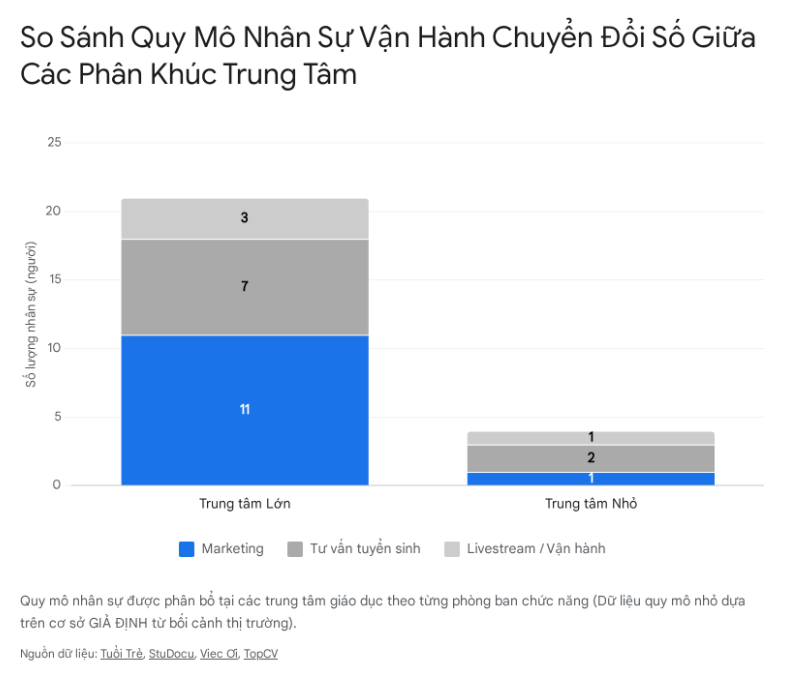
\includegraphics[width=0.85\linewidth]{imgs/PA3_pics/image2_v3.png}
    \caption{So sánh mô hình nhân sự giữa trung tâm quy mô lớn và trung tâm nhỏ}
    \label{fig:pa3_staffing_comparison}
\end{figure}

\paragraph{5. Nội dung nào thường xuyên bị lặp lại trong các phiên tiếp thị?}

Hành trình khách hàng (Customer Journey) trong mảng giáo dục đào tạo, đặc biệt là việc đăng ký các khóa học ngôn ngữ, là một chuỗi quyết định đòi hỏi sự cân nhắc kỹ lưỡng (high-involvement decision). Tuy nhiên, vòng đời ra quyết định của học viên thường bắt đầu bằng vô số các truy vấn mang tính thông tin cơ bản trước khi họ thực sự chuyển sang giai đoạn cân nhắc và mua hàng. Phân tích dữ liệu học thuật, hoạt động tư vấn và các luồng bình luận trên mạng xã hội cho thấy các nhóm nội dung bị lặp lại với tần suất dày đặc nhất bao gồm:

\begin{enumerate}
    \item \textbf{Học phí (Tuition Fees):} Đây là câu hỏi kinh điển, phổ biến nhất và có tính cấu trúc cao nhất. Bất chấp việc thông tin có thể đã được ghim trên màn hình, học viên vẫn liên tục hỏi trên livestream hoặc chat. Mức độ phức tạp của câu hỏi này nằm ở chỗ học phí có độ dao động rất lớn. Chẳng hạn, khảo sát cho thấy học phí các khóa IELTS thường dao động từ 5.920.000 VNĐ đến 17.000.000 VNĐ tùy theo lộ trình và đầu vào.\footnote{Khoá học IELTS cơ bản, học phí từ 5.920.000 -- Trung tâm Ngoại ngữ ECE, accessed July 17, 2026, \url{https://ece.edu.vn/1-khoa-hoc-ielts-bao-nhieu-tien/}} Thậm chí, các khóa học kèm 1-1 cấp tốc có thể lên tới 28.800.000 VNĐ đến 44.000.000 VNĐ.\footnote{Khoá học IELTS cơ bản, học phí từ 5.920.000 -- Trung tâm Ngoại ngữ ECE, accessed July 17, 2026, \url{https://ece.edu.vn/1-khoa-hoc-ielts-bao-nhieu-tien/}}
    \item \textbf{Lịch học / Lịch khai giảng (Schedules):} Khách hàng luôn có nhu cầu đối chiếu lịch trình cá nhân của họ (lịch làm việc, lịch học tại trường đại học) với lịch khai giảng của trung tâm.\footnote{[Mới Nhất] TOP 10 TRUNG TÂM TIẾNG ANH CHO NGƯỜI ĐI LÀM TẠI ĐÀ NẴNG, accessed July 17, 2026, \url{https://wiseenglish.edu.vn/trung-tam-tieng-anh-cho-nguoi-di-lam}} Việc tư vấn viên phải liên tục dò tìm bảng Excel để thông báo ``lớp 3-5-7 tối 19h đã đầy, mời bạn chuyển sang lớp 2-4-6'' lặp lại hàng trăm lần mỗi ngày.
    \item \textbf{Yêu cầu Đầu vào / Đầu ra (Input/Output Requirements):} Các chứng chỉ quốc tế uy tín đều yêu cầu nghiêm ngặt về bài kiểm tra năng lực đầu vào xếp lớp (Placement Test) và những cam kết chắc chắn về đầu ra (ví dụ: IELTS 6.5+, TOEIC 900+).\footnote{Học phí tại Langmaster bao nhiêu tiền? Bảng giá các khóa học, accessed July 17, 2026, \url{https://langmaster.edu.vn/cap-nhat-moi-nhat-hoc-phi-langmaster-hien-nay-co-gia-bao-nhieu}} Học viên liên tục hỏi những câu như: ``Em mất gốc thì học bao lâu đạt IELTS 6.5?'', ``Đầu vào của khóa IELTS Intermediate là bao nhiêu?''.
    \item \textbf{Chính sách, Phương pháp \& Ưu đãi (Policies \& Promotions):} Câu hỏi xoay quanh việc học thử miễn phí, giảm giá nhân dịp sự kiện, chính sách hoàn tiền (Refund policy) trong trường hợp không đạt cam kết đầu ra, hoặc bảo lưu khóa học diễn ra liên tục.\footnote{[Mới Nhất] TOP 10 TRUNG TÂM TIẾNG ANH CHO NGƯỜI ĐI LÀM TẠI ĐÀ NẴNG, accessed July 17, 2026, \url{https://wiseenglish.edu.vn/trung-tam-tieng-anh-cho-nguoi-di-lam}} Học viên cũng hay thắc mắc về phương pháp học (Ví dụ: phương pháp NLP tiết kiệm 80\% thời gian\footnote{[Mới Nhất] TOP 10 TRUNG TÂM TIẾNG ANH CHO NGƯỜI ĐI LÀM TẠI ĐÀ NẴNG, accessed July 17, 2026, \url{https://wiseenglish.edu.vn/trung-tam-tieng-anh-cho-nguoi-di-lam}}).
\end{enumerate}

Sự lặp lại không hồi kết của các câu hỏi này tạo ra một điểm nghẽn (bottleneck) trầm trọng trong vận hành. Nhân viên phòng ban thường xuyên phải trả lời các câu hỏi lặp đi lặp lại một cách máy móc, gây tốn kém tài nguyên nhân sự vô ích.\footnote{Học Viên Hỏi -- Chatbot Trả Lời: Gỡ Tắc Nghẽn Thông Tin Học Vụ -- NIXXIS, accessed July 17, 2026, \url{https://nixxis.vn/chatbot-tu-van-hoc-vu-cho-hoc-vien/}} Hậu quả của tình trạng tắc nghẽn thông tin học vụ này là tạo ra sự mệt mỏi, căng thẳng (burnout) cho đội ngũ, giảm hiệu suất làm việc chung, khiến họ không thể tập trung trí lực vào các nhiệm vụ phức tạp hơn như thuyết phục khách hàng ở chặng cuối. Nguy hiểm hơn, sự chậm trễ trong phản hồi do quá tải dẫn đến việc bỏ lỡ cơ hội chốt đơn, rơi rụng khách hàng tiềm năng.\footnote{Học Viên Hỏi -- Chatbot Trả Lời: Gỡ Tắc Nghẽn Thông Tin Học Vụ -- NIXXIS, accessed July 17, 2026, \url{https://nixxis.vn/chatbot-tu-van-hoc-vu-cho-hoc-vien/}}

Chính vì vậy, việc triển khai một cơ chế tự động hóa chuỗi câu trả lời này thông qua hệ thống AI Sales Agent -- có khả năng truy xuất ngay lập tức bảng giá, lịch học và chính sách dựa trên RAG -- không chỉ là một tiện ích bổ sung (nice-to-have), mà là một giá trị cốt lõi (must-have) giải quyết đúng điểm đau nhức nhối nhất trong vận hành của các trung tâm.

%% ================================================================
%% PHẦN 1 (tiếp): CHÂN DUNG NGƯỜI MUA HÀNG
%% ================================================================
\subsubsection{Chân dung Người MUA HÀNG (Buying Persona)}

Trong môi trường bán hàng B2B (Doanh nghiệp với Doanh nghiệp) của lĩnh vực EdTech, chiến lược Tiếp cận thị trường (GTM) thành công phải bắt đầu từ việc thấu hiểu sâu sắc người nắm giữ ngân sách và quyền ký quyết định giải ngân. Trong hệ sinh thái giáo dục, nhân vật quyền lực này chính là Chủ trung tâm, Người sáng lập hoặc Giám đốc/Quản lý chi nhánh.

\textbf{Hồ sơ đại diện (Profile):} Chủ đầu tư / Giám đốc Trung tâm Ngoại ngữ / Giám đốc Vận hành chuỗi Giáo dục.

\begin{itemize}
    \item \textbf{Mục tiêu kinh doanh (Business Goals):}
    \begin{itemize}
        \item Tối đa hóa doanh thu tuyển sinh từ các nền tảng trực tuyến, đặc biệt là nắm bắt kịp thời xu hướng Video Commerce và Livestream (đang đóng góp tỷ trọng sống còn vào GMV bán lẻ trực tuyến tại Đông Nam Á và Việt Nam).\footnote{Nguồn: [CSH2026][1Stream][FINAL PITCH DECK].pdf}
        \item Giảm thiểu chi phí trên mỗi khách hàng tiềm năng (Cost Per Lead -- CPL) và tối ưu hóa hệ số thu nhập trên đầu tư (ROI). Cốt lõi của mục tiêu này là mở rộng quy mô hoạt động, duy trì hình ảnh thương hiệu nhất quán 24/7 mà không làm phình to quỹ lương sự một cách mất kiểm soát.
    \end{itemize}
    \item \textbf{Vấn đề / Nỗi đau (Pain Points):}
    \begin{itemize}
        \item Gánh nặng tài chính khổng lồ từ chi phí nhân sự, chiếm tới 50--60\% ngân sách vận hành.\footnote{Nguồn: [CSH2026][1Stream][FINAL PITCH DECK].pdf} Đặc biệt là các khoản tiền lương phải trả thêm cho nhân viên trực đêm ngoài giờ hành chính, hoặc chi phí khổng lồ để thuê các Host livestream chuyên nghiệp (với mức lương trung bình 15--25 triệu/tháng, thậm chí 50 triệu/tháng).\footnote{Tuyển dụng 413 việc làm Vận hành Livestream [Update 15/07/2026] -- TopCV, accessed July 17, 2026, \url{https://www.topcv.vn/tim-viec-lam-van-hanh-livestream-cr1cb8cl618}}
        \item Sự biến động nhân sự (Turnover rate) rất lớn trong ngành giáo dục, đặc biệt ở bộ phận Telesales và trực page do áp lực công việc, dẫn đến chi phí tuyển dụng và đào tạo lại không ngừng phát sinh.
        \item Hiệu suất tư vấn giảm mạnh (lead response time chậm) trong các khung giờ cao điểm hoặc ban đêm khi lượng bình luận tăng đột biến, dẫn đến tỷ lệ rớt khách (lead drop-off) cao, lãng phí chi phí marketing (Ad spend).
    \end{itemize}
    \item \textbf{Rào cản mua hàng (Barriers):}
    \begin{itemize}
        \item \textit{Rào cản kỹ thuật \& Vận hành:} Hoài nghi sâu sắc về khả năng tích hợp của công nghệ AI vào quy trình (workflow) hiện hành. Lo sợ việc áp dụng phần mềm mới sẽ yêu cầu thời gian đào tạo dài, gây xáo trộn và làm gián đoạn luồng vận hành đang ổn định của trung tâm.
        \item \textit{Rủi ro thương hiệu:} Ám ảnh với việc AI có thể ``ảo giác'' (hallucinate) và cung cấp thông tin sai lệch cho khách hàng về học phí, cam kết điểm số, gây ra khủng hoảng truyền thông hoặc các rắc rối về pháp lý, hợp đồng.\footnote{Nguồn: [CSH2026][1Stream][FINAL PITCH DECK].pdf}
        \item \textit{Bảo mật \& Quyền riêng tư:} Sự e ngại về việc bảo mật cơ sở dữ liệu khách hàng (lead data) và tài liệu nội bộ khi giao phó cho một nền tảng bên thứ ba.
    \end{itemize}
    \item \textbf{Tiêu chí quyết định mua (Buying Criteria):}
    \begin{itemize}
        \item Giải pháp phải chứng minh được việc cắt giảm chi phí (Cost-Effective) một cách minh bạch, có các số liệu dự phóng dòng tiền rõ ràng và khả năng đo lường hiệu quả ngay trong tháng đầu tiên sử dụng. Phải có lộ trình hoàn vốn (Payback period) ngắn hạn.
        \item Hệ thống yêu cầu thời gian triển khai và mang lại giá trị (Time-to-value / Onboarding) cực ngắn, cắm-và-chạy (plug-and-play).
        \item Phải có cam kết bằng văn bản hoặc bằng chứng kỹ thuật vững chắc (ví dụ: công nghệ RAG) về tính chính xác tuyệt đối của AI khi phản hồi, dựa trên dữ liệu chuẩn hóa của riêng trung tâm.
    \end{itemize}
    \item \textbf{Kênh tiếp nhận thông tin thường xuyên (Preferred Information Channels):}
    \begin{itemize}
        \item Gặp gỡ trực tiếp thông qua các buổi họp cấp cao, tham dự các hội thảo quy mô về giáo dục, hội thảo công nghệ giáo dục (như Triển lãm Edtech Expo) nơi tập trung các xu hướng mới nhất.\footnote{Việt Nam nằm trong top 10 thị trường EdTech thế giới, top 3 thị trường Đông Nam Á, accessed July 17, 2026, \url{https://vneconomy.vn/techconnect/viet-nam-nam-trong-top-10-thi-truong-edtech-the-gioi-top-3-thi-truong-dong-nam-a.htm}}
        \item Kênh mạng xã hội nghề nghiệp LinkedIn, đặc biệt nhắm mục tiêu vào các bài viết lãnh đạo tư tưởng (Thought Leadership) dành cho các chức danh ``Giám đốc vận hành'', ``Founder'', ``CEO'' trong ngành giáo dục.
        \item Lắng nghe sự giới thiệu, truyền miệng (Referral/Word-of-mouth) từ mạng lưới cộng đồng quản lý giáo dục và các đối tác trong ngành.
    \end{itemize}
\end{itemize}

%% ================================================================
%% PHẦN 2: CHÂN DUNG NGƯỜI DÙNG TRỰC TIẾP
%% ================================================================
\subsubsection{Phần 2: Chân dung Người DÙNG TRỰC TIẾP (User Persona)}

Thành bại của một chiến lược SaaS không chỉ phụ thuộc vào cái gật đầu của người ký séc, mà còn được quyết định bởi tỷ lệ chấp nhận sản phẩm (Adoption Rate) của người dùng cuối. Những nhân sự dưới đây là những người trực tiếp ``nhúng tay'' vào nền tảng mỗi ngày. Việc GTM phải giải quyết được triệt để nỗi đau tâm lý của họ.

\paragraph{Persona 2.1: Trưởng phòng Marketing (Người bảo trợ nội bộ -- Internal Sponsor)}

\begin{itemize}
    \item \textbf{Hành vi \& Trách nhiệm:} Là người đầu tàu chịu trách nhiệm lập kế hoạch, phân bổ ngân sách quảng cáo, tổ chức các sự kiện livestream quy mô lớn, thiết lập các chiến dịch tạo khách hàng tiềm năng (Lead Generation) và giám sát hiệu quả của mọi kênh truyền thông (Digital Marketing).\footnote{CÔNG TY TRÁCH NHIỆM HỮU HẠN TRUNG TÂM NGOẠI NGỮ AMA VŨNG TÀU tuyển dụng Trưởng phòng Tư vấn tuyển sinh -- UEH Youth, accessed July 17, 2026, \url{https://youth.ueh.edu.vn/ho-tro-sinh-vien-2/cong-ty-trach-nhiem-huu-han-trung-tam-ngoai-ngu-ama-vung-tau-tuyen-dung-truong-phong-tu-van-tuyen-sinh/}} Họ liên tục theo dõi báo cáo phân tích số liệu (analytics).
    \item \textbf{Vấn đề (Pain Points):} Luôn phải vật lộn trong việc chứng minh hiệu quả đầu tư (ROI) của các phiên livestream với Ban Giám đốc do không thể đo lường chính xác lượng khách hàng tiềm năng bị bỏ sót qua bình luận. Chịu áp lực nặng nề trong việc phải sản xuất nội dung liên tục (video ngắn, kịch bản live đa nền tảng) nhưng luôn trong tình trạng thiếu hụt ý tưởng sáng tạo và nhân lực thực thi.\footnote{Nguồn: [CSH2026][1Stream][FINAL PITCH DECK].pdf} Đội ngũ dưới quyền thường xuyên bị quá tải khi phải điều phối chéo giữa bộ phận làm content và bộ phận trực page, chốt sales.
    \item \textbf{Tiêu chí quyết định ủng hộ:}
    \begin{itemize}
        \item Nền tảng phải cung cấp một hệ thống Dashboard Analytics trực quan, báo cáo tự động theo thời gian thực (Real-time tracking) để họ dễ dàng xuất báo cáo gửi Giám đốc.
        \item Tính năng tích hợp mượt mà với các nền tảng mạng xã hội đang sử dụng (TikTok, Facebook, Shopee, YouTube) mà không phá vỡ quy trình hiện tại.
        \item Đặc biệt quan tâm đến tính năng AI Video/Script Generator giúp tự động hóa kịch bản, giảm thiểu thời gian sản xuất nội dung đa kênh.\footnote{Nguồn: [CSH2026][1Stream][FINAL PITCH DECK].pdf}
    \end{itemize}
\end{itemize}

\paragraph{Persona 2.2: Nhân viên / Quản lý Tư vấn Tuyển sinh (Direct User)}

\begin{itemize}
    \item \textbf{Hành vi \& Trách nhiệm:} Trực tiếp tư vấn các khóa học tiếng Anh, chứng chỉ quốc tế; duy trì liên lạc với phụ huynh và học viên qua tin nhắn, điện thoại (Telesales). Họ là những ``chiến binh'' thực thi, đảm bảo đạt chỉ tiêu doanh số cá nhân (KPI) hàng tháng.\footnote{Tuyển Nhân Viên Tư Vấn Giáo Dục làm việc tại TRUNG TÂM ANH NGỮ EASY EDU, accessed July 17, 2026, \url{https://www.topcv.vn/viec-lam/nhan-vien-tu-van-giao-duc/1562009.html}}
    \item \textbf{Vấn đề (Pain Points):} Bị vắt kiệt sức lực và thời gian khi phải lặp đi lặp lại hàng trăm lần mỗi ngày những câu trả lời khô khan về ``Học phí IELTS bao nhiêu?'', ``Lịch học tuần này thế nào?''. Sự quá tải từ những câu hỏi rác (junk queries) này tước đi thời gian quý báu để họ phát huy nghệ thuật thuyết phục (closing skills) đối với những khách hàng đang ở chặng cuối của phễu mua hàng. Thường xuyên rơi vào trạng thái căng thẳng tột độ, mệt mỏi trong các mùa cao điểm tuyển sinh.\footnote{Học Viên Hỏi -- Chatbot Trả Lời: Gỡ Tắc Nghẽn Thông Tin Học Vụ -- NIXXIS, accessed July 17, 2026, \url{https://nixxis.vn/chatbot-tu-van-hoc-vu-cho-hoc-vien/}}
    \item \textbf{Tiêu chí quyết định ủng hộ:}
    \begin{itemize}
        \item Đòi hỏi phần mềm có khả năng phân luồng thông minh, chỉ chuyển giao cho họ những cuộc hội thoại thực sự có ``ý định mua hàng'' (high-intent) hoặc các ca phức tạp (khách hàng phàn nàn, cần tư vấn lộ trình cá nhân hóa).
        \item Giao diện quản lý chat tập trung, đơn giản, ít thao tác (click). Không muốn phải đối mặt với một hệ thống CRM quá phức tạp bắt buộc phải học lại từ đầu.
    \end{itemize}
\end{itemize}

\paragraph{Persona 2.3: Nhân viên / Host Vận hành Livestream (Direct User)}

\begin{itemize}
    \item \textbf{Hành vi \& Trách nhiệm:} Họ là bộ mặt của trung tâm trên mạng xã hội. Trách nhiệm bao gồm chuẩn bị kịch bản, trực tiếp đứng trước ống kính dẫn dắt (đối với host), hoặc tinh chỉnh phần mềm phát sóng, âm thanh, ánh sáng (đối với nhân sự vận hành). Suốt quá trình live, họ phải đọc, lọc và phản hồi bình luận theo thời gian thực.\footnote{Giáo viên Tiếng Anh Host Livestream -- Joboko, accessed July 17, 2026, \url{https://vn.joboko.com/viec-lam-giao-vien-tieng-anh-host-livestream-xvi6575019?amp=1}}
    \item \textbf{Vấn đề (Pain Points):} Chịu áp lực tâm lý và thể chất cực lớn khi phải livestream liên tục nhiều giờ đồng hồ, đặc biệt là phải làm việc vào các khung giờ thấp điểm, ngoài giờ hành chính hoặc ban đêm (ví dụ: các phiên live bắt đầu từ 20:00).\footnote{Chi chục triệu học livestream bán hàng -- Báo Tuổi Trẻ, accessed July 17, 2026, \url{https://tuoitre.vn/nld/chi-chuc-trieu-hoc-livestream-ban-hang-196231203114313834.htm}} Thường xuyên bị phân tâm tâm lý do não bộ phải xử lý đa luồng (multi-tasking): vừa phải duy trì ngữ điệu, hình thể, vừa phải nheo mắt đọc và tương tác với hàng ngàn bình luận trôi qua màn hình.
    \item \textbf{Tiêu chí quyết định ủng hộ:}
    \begin{itemize}
        \item Công cụ giúp giảm tải công việc rõ rệt, chẳng hạn như kịch bản tự động chạy, màn hình nhắc chữ thông minh, hoặc khả năng sử dụng avatar AI hỗ trợ duy trì luồng phát sóng trong các khung giờ mệt mỏi.\footnote{Nguồn: [CSH2026][1Stream][FINAL PITCH DECK].pdf}
        \item Cơ chế AI lọc và trả lời bình luận tự động giúp họ an tâm, không sợ lỡ khách, từ đó có thể toàn tâm toàn ý tập trung vào chuyên môn giảng dạy hoặc dẫn dắt cảm xúc người xem, thay vì phải liên tục dừng lại để báo giá.
    \end{itemize}
\end{itemize}

\paragraph{Persona 2.4: Bộ phận Học vụ / Người Cung cấp dữ liệu (Data Provider)}

\begin{itemize}
    \item \textbf{Hành vi \& Trách nhiệm:} Xây dựng, biên soạn giáo trình chuẩn quốc tế, quy định chính sách bảo lưu, sắp xếp thời khóa biểu. Đảm bảo thông tin đào tạo được truyền đạt đồng nhất, tuân thủ nghiêm ngặt các quy chuẩn học thuật.\footnote{Việc làm Nhân viên tư vấn trung tâm ngoại ngữ -- Indeed, accessed July 17, 2026, \url{https://vn.indeed.com/q-nh\%C3\%A2n-vi\%C3\%AAn-t\%C6\%B0-v\%E1\%BA\%A5n-trung-t\%C3\%A2m-ngo\%E1\%BA\%A1i-ng\%E1\%BB\%AF-vi\%E1\%BB\%87c-l\%C3\%A0m.html}}
    \item \textbf{Vấn đề (Pain Points):} Phải liên tục cập nhật thông tin một cách thủ công mỗi khi trung tâm có thay đổi về lịch khai giảng hay giá học phí. Vô cùng bất bình và phàn nàn khi nhân viên sales tư vấn sai lệch hoặc ``hứa lèo'' về cam kết đầu ra (ví dụ: cam kết IELTS 8.0 trong 1 tháng) chỉ để chốt được đơn.
    \item \textbf{Tiêu chí quyết định ủng hộ:}
    \begin{itemize}
        \item Quy trình tải lên (upload) và đồng bộ dữ liệu khóa học vào bộ não AI phải cực kỳ đơn giản, không cần kỹ năng code (Ví dụ: chỉ cần kéo thả file Excel, PDF, bảng giá sẵn có).
        \item Hệ thống AI phải được giới hạn bởi các ``guardrails'' (rào chắn) nghiêm ngặt, đảm bảo phản hồi dựa trên tập tài liệu (Knowledge Base) một cách tuyệt đối trung thành, không bao giờ tự ý sáng tạo thông tin ngoài luồng.
    \end{itemize}
\end{itemize}

%% ================================================================
%% PHẦN 3: BẢNG BUYING CENTER
%% ================================================================
\subsubsection{Phần 3: Bảng Đơn vị Ra Quyết định mua (Buying Center) dưới Lăng kính GTM}

Để chuyển đổi thành công một khách hàng doanh nghiệp B2B trong mảng giáo dục, thông điệp truyền thông không thể dùng chung một kịch bản. Việc thuyết phục (Pitching) phải được cá nhân hóa sâu sắc theo ngôn ngữ của từng vị trí. Dựa trên cấu trúc 5 vai trò (PA2), dưới đây là Bảng Buying Center được tái thiết kế và mở rộng dưới góc nhìn chiến lược Tiếp cận thị trường (GTM). Mục tiêu không chỉ là xác định \textit{Ai mua, Ai dùng, Ai cản}, mà là \textit{Nói cái gì (Message)} và \textit{Nói qua kênh nào (Channel)} để đạt được sự đồng thuận từ từng nút thắt trong mạng lưới nhân sự phức tạp của khách hàng.

\begin{table}[H]
    \centering
    \footnotesize
    \setlength{\tabcolsep}{3pt}
    \renewcommand{\arraystretch}{1.25}
    \caption{Bảng Đơn vị Ra Quyết định mua (Buying Center) dưới Lăng kính GTM}
    \label{tab:buying_center_gtm}
    \rowcolors{2}{paperBg}{white}
    \begin{tabularx}{\linewidth}{@{} c L{2.2cm} L{2.5cm} L{3cm} Y L{2.8cm} @{}}
        \toprule
        \rowcolor{softBlue}
        \textbf{\#} & \textbf{Vai trò} & \textbf{Chức danh} & \textbf{Mối quan tâm chính} & \textbf{Thông điệp Marketing} & \textbf{Kênh tiếp cận} \\ \midrule
        %
        \textbf{1} & Người duyệt ngân sách (Budget Approver) & Chủ trung tâm, Giám đốc, Quản lý chi nhánh & Chi phí đầu tư, hiệu quả tuyển sinh, rủi ro tổn hại thương hiệu và khả năng mua lại (Retention). & \textbf{Thông điệp ROI \& Tối ưu chi phí:} ``Cắt giảm ngay 50\% chi phí quỹ lương cho nhân sự trực page ngoài giờ. Khả năng duy trì hoạt động bán hàng livestream 24/7. Giảm CPL (Cost Per Lead) gấp 3 lần với tỷ lệ hoàn vốn trong chưa đầy 3 tháng.'' Kèm theo các Case Study thực chứng từ các trung tâm giáo dục có cùng quy mô. & Gặp gỡ trực tiếp (On-site B2B Demo, Executive meetings); Chạy quảng cáo LinkedIn Ads nhắm mục tiêu chức danh ``Giám đốc trung tâm đào tạo'', ``CEO EdTech''; Triển lãm EdTech Expo; Giới thiệu qua mạng lưới đối tác (Referral). \\ \midrule
        %
        \textbf{2} & Người bảo trợ nội bộ (Internal Sponsor) & Trưởng phòng Marketing, Trưởng phòng Tư vấn Tuyển sinh, Quản lý Vận hành & Cần một giải pháp giải quyết ngay tình trạng quá tải, dễ dàng phối hợp với đội ngũ hiện tại mà không làm gián đoạn hệ thống, cần số liệu trực quan để báo cáo cấp trên. & \textbf{Thông điệp Hiệu suất \& Tự động hóa:} ``Tự động hóa kịch bản đa kênh, làm chủ dữ liệu luồng hội thoại. Cung cấp Dashboard báo cáo số lượng lead/bình luận đã xử lý theo thời gian thực. Tích hợp cực nhanh, cắm-và-chạy không phá vỡ quy trình hiện tại của đội ngũ.'' & Email marketing chuyên sâu (Bản tin chiến lược ngành); Tin nhắn Zalo ZNS; Các buổi Webinar chia sẻ kiến thức kết hợp Demo tính năng; Hoạt động trong các cộng đồng Quản trị Marketing \& Tuyển sinh giáo dục. \\ \midrule
        %
        \textbf{3} & Người sử dụng trực tiếp (Direct User) & Nhân viên/Host Livestream, Chuyên viên Tư vấn (Telesales), Nhân viên Content & Đòi hỏi phần mềm phải dễ sử dụng, cực ít thao tác click. Muốn nội dung AI tư vấn phải chính xác. Cần cơ chế chuyển giao linh hoạt các câu hỏi khó cho người thật. Sợ công nghệ thay thế mình. & \textbf{Thông điệp Hỗ trợ \& Đồng hành:} ``Bạn không cần học thêm công cụ mới --- chỉ cần bật và Trợ lý AI tự chạy. AI giúp bạn giải phóng khỏi hàng ngàn bình luận hỏi giá lặp đi lặp lại để bạn tập trung vào nghệ thuật chốt sales và thỏa sức sáng tạo. Giảm tải hoàn toàn việc trực đêm.'' & Video hướng dẫn ngắn gọn, giải trí (TikTok, Reels) mang tính viral về nỗi đau ngành sales; Trải nghiệm dùng thử miễn phí (Free trial / Hands-on); Nhóm cộng đồng hỗ trợ Zalo/Facebook; Hệ thống In-app tutorials (hướng dẫn ngay trong phần mềm). \\ \midrule
        %
        \textbf{4} & Người cung cấp dữ liệu (Data Provider) & Trưởng phòng Đào tạo, Giáo viên, Học vụ, Cán bộ Hành chính & Yêu cầu khắt khe về tính chính xác của thông tin học thuật, lịch học, bảng giá học phí và chính sách. Sợ AI cung cấp thông tin sai lệch gây hậu quả. & \textbf{Thông điệp Chính xác tuyệt đối:} ``Hệ thống chỉ trả lời đúng những gì bạn dạy nó. Công nghệ RAG đảm bảo AI trung thành 100\% với tài liệu gốc. Không bịa đặt thông tin. Quá trình nhập liệu siêu đơn giản: Chỉ cần kéo thả 1 lần file Excel/Word/Bảng giá, hệ thống tự động chuẩn hóa.'' & Các buổi Onboarding call trực tiếp (1-on-1) để hướng dẫn kỹ thuật; Cung cấp các bộ tài liệu Hướng dẫn nhập liệu (có Template Excel chuẩn sẵn); Hỗ trợ kỹ thuật qua email/Zalo với tốc độ phản hồi tính bằng phút. \\ \midrule
        %
        \textbf{5} & Người có thể phản đối (Objector) & Bộ phận Pháp chế (Legal), Quản trị rủi ro Thương hiệu, Quản trị tài khoản MXH & Cảnh giác cao độ về quyền bảo mật dữ liệu, quyền sử dụng hình ảnh/giọng nói. Lo sợ vi phạm tiêu chuẩn cộng đồng và tuân thủ chính sách khắt khe của các nền tảng (Facebook, TikTok). & \textbf{Thông điệp An toàn, Bảo mật \& Tuân thủ:} ``Cam kết mã hóa và bảo mật dữ liệu đầu cuối. Hợp đồng sử dụng bản quyền hình ảnh, giọng nói rõ ràng, minh bạch. Nền tảng tuân thủ 100\% chính sách của Facebook/TikTok. Có cơ chế kiểm duyệt trước (bước duyệt nội dung AI) nhằm ngăn chặn rủi ro.'' & Gửi các Bộ tài liệu pháp lý minh bạch (Terms of Service, NDA); Sách trắng (Whitepaper) về kiến trúc bảo mật của nền tảng; Thực hiện các buổi Demo cơ chế kiểm duyệt nội dung của AI trực tiếp cho bộ phận pháp chế đánh giá. \\ \bottomrule
    \end{tabularx}
    \rowcolors{2}{}{}
\end{table}

%% ================================================================
%% PHÂN TÍCH CHIẾN LƯỢC THỰC THI GTM
%% ================================================================
\subsubsection{Phân tích Chiến lược Thực thi GTM (GTM Execution Strategy)}

Để thương mại hóa thành công một nền tảng SaaS ứng dụng AI như 1Stream vào môi trường giáo dục đầy bảo thủ nhưng cũng rất khao khát công nghệ, chiến lược GTM không thể áp dụng tư duy ``một thông điệp bán cho tất cả'' (one-size-fits-all). Sự phức tạp trong quy trình nội bộ của các trung tâm đòi hỏi một cách tiếp cận B2B đa tầng, thâm nhập từ dưới lên và chốt hạ từ trên xuống.

\textbf{1. Xây dựng Phễu Tiếp cận (The Approach Funnel):} Chiến dịch marketing sẽ khởi đầu bằng việc thu hút sự chú ý của \textbf{Người bảo trợ nội bộ} (Trưởng Marketing/Tuyển sinh) thông qua việc phát hành các báo cáo phân tích thực trạng về ``Sự lãng phí chi phí vận hành Livestream trong Giáo dục'' (được lan truyền trên LinkedIn và các cộng đồng chuyên môn). Khi Người bảo trợ đã thấu cảm nỗi đau và nhận thấy giải pháp, họ sẽ chính là ``đại sứ thương hiệu'' nội bộ, mang sản phẩm đi thuyết phục \textbf{Người duyệt ngân sách} (Giám đốc). Do đó, bộ phận Bán hàng B2B (B2B Sales) của giải pháp AI cần vũ trang cho vị Trưởng Marketing này một ``Bộ công cụ thuyết phục nội bộ'' (Internal Pitch Deck) bao gồm: bảng phân tích tài chính vi mô, mô hình dự phóng ROI tính toán được lượng tiền lương tiết kiệm, và bộ cam kết bảo mật rủi ro.

\textbf{2. Định vị Chiến lược Dựa trên Phân khúc Quy mô (Size-Based Positioning):}

\begin{itemize}
    \item \textbf{Thị trường Ngách Khởi điểm (Micro-seller / Trung tâm siêu nhỏ / Cá nhân):} Ở phân khúc này, chu kỳ ra quyết định cực kỳ ngắn gọn. Vị Giám đốc thường kiêm luôn vai trò Trưởng Marketing, Telesales và Học vụ. Thông điệp GTM tại đây phải đánh mạnh vào cảm xúc và sinh tồn: ``Công cụ giá rẻ, thiết lập trong 15 phút, giải phóng sức lao động, lấy lại giấc ngủ ban đêm''.\footnote{Nguồn: [CSH2026][1Stream][FINAL PITCH DECK].pdf}
\end{itemize}

\begin{WarningBox}[GIẢ ĐỊNH]
Chi phí là yếu tố nhạy cảm bậc nhất ở quy mô này, chiến lược giá cần tiếp cận bằng các gói Freemium (miễn phí tính năng cơ bản) hoặc Starter với giá thuê bao cực thấp, rào cản tài chính bằng không.
\end{WarningBox}

\begin{itemize}
    \item \textbf{Thị trường Mục tiêu Chính (SME \& Các hệ thống giáo dục lớn):} Nhóm này sở hữu cấu trúc nhân sự phân mảnh rõ rệt thành 5 vai trò như đã phân tích. Chiến lược GTM phải lập tức chuyển hướng sang bán hàng B2B truyền thống chuyên sâu. Đòi hỏi việc thiết lập các cuộc gặp gỡ cấp cao (Executive Meetings), thực hiện Demo sản phẩm tận nơi (On-site) dựa trên chính dữ liệu thật của trung tâm, và cung cấp các bản Cam kết chất lượng dịch vụ (SLA -- Service Level Agreement) vững chắc.\footnote{Nguồn: [CSH2026][1Stream][FINAL PITCH DECK].pdf}
\end{itemize}

\textbf{3. Xóa bỏ rào cản bằng Lợi thế Kỹ thuật (The RAG Advantage):} Vũ khí GTM mạnh nhất để dập tắt sự phản đối từ nhóm \textbf{Người cung cấp dữ liệu} và \textbf{Người có thể phản đối} là đẩy mạnh truyền thông và giáo dục thị trường về công nghệ RAG (Retrieval-Augmented Generation). Thay vì nói chung chung ``AI rất thông minh'', thông điệp cần mang tính kỹ thuật nhưng dễ hiểu: Việc nhấn mạnh rằng AI LLM sẽ bị ``nhốt'' trong một khung tri thức cố định, chỉ xử lý 100\% các câu hỏi về \textit{học phí, lịch học, đầu vào} dựa trên bảng biểu JSON có sẵn sẽ lập tức tạo được sự an tâm tuyệt đối về mặt học thuật và loại bỏ rủi ro pháp lý.\footnote{Nguồn: [CSH2026][1Stream][FINAL PITCH DECK].pdf}

Tựu trung lại, sự thành công của một chiến dịch GTM trong mảng EdTech SaaS nằm ở nghệ thuật giao tiếp đa diện. Giải pháp công nghệ phải biết cách nói chuyện đồng thời với một vị Giám đốc đang khao khát tối ưu hóa ROI, một vị Trưởng phòng Marketing đang khát khao báo cáo hiệu suất đẹp, và một người Nhân viên Tư vấn đang rã rời mong mỏi được giải phóng khỏi những tác vụ lặp lại nhàm chán mỗi đêm. Khi thiết kế thông điệp tùy chỉnh cho từng điểm chạm, sản phẩm sẽ dễ dàng phá vỡ lớp vỏ bọc phòng thủ, tiến tới tích hợp sâu rộng vào quy trình cốt lõi của doanh nghiệp giáo dục.

%% ================================================================
%% WORKS CITED (danh sách 27 nguồn tham khảo)
%% ================================================================
% 1.  Việt Nam nằm trong top 10 thị trường EdTech thế giới, top 3 thị trường Đông Nam Á,
%     accessed July 17, 2026,
%     https://vneconomy.vn/techconnect/viet-nam-nam-trong-top-10-thi-truong-edtech-the-gioi-top-3-thi-truong-dong-nam-a.htm
% 2.  Quy mô thị trường giáo dục trực tuyến K-12, Báo cáo xu hướng ngành,
%     accessed July 17, 2026,
%     https://www.forinsightsconsultancy.com/vi/báo-cáo/thị-trường-giáo-dục-trực-tuyến-k-12
% 3.  [CSH2026][1Stream][FINAL PITCH DECK].pdf
% 4.  Sách trắng EdTech Việt Nam 2025 | PDF – Scribd,
%     accessed July 17, 2026,
%     https://www.scribd.com/document/996258987/Sa-ch-tra-ng-EdTech-Việt-Nam-2025
% 5.  Cấu trúc nhân sự trung tâm ngoại ngữ: Giám đốc, giáo viên và các bộ phận chuyên môn,
%     accessed July 17, 2026,
%     https://luatminhthinh.vn/cau-truc-nhan-su-trung-tam-ngoai-ngu-giam-doc-giao-vien-va-cac-bo-phan-chuyen-mon/
% 6.  Điều kiện của bộ máy nhân sự trung tâm ngoại ngữ – Luật Thành Đô,
%     accessed July 17, 2026,
%     https://luatthanhdo.com.vn/dieu-kien-cua-bo-may-nhan-su-trung-tam-ngoai-ngu
% 7.  Giáo viên Tiếng Anh Host Livestream – Joboko,
%     accessed July 17, 2026,
%     https://vn.joboko.com/viec-lam-giao-vien-tieng-anh-host-livestream-xvi6575019?amp=1
% 8.  Giáo viên Tiếng Anh Host Livestream – Joboko,
%     accessed July 17, 2026,
%     https://vn.joboko.com/viec-lam-giao-vien-tieng-anh-host-livestream-xvi6575019
% 9.  Tuyển dụng 413 việc làm Vận hành Livestream [Update 15/07/2026] – TopCV,
%     accessed July 17, 2026,
%     https://www.topcv.vn/tim-viec-lam-van-hanh-livestream-cr1cb8cl618
% 10. CÔNG TY TRÁCH NHIỆM HỮU HẠN TRUNG TÂM NGOẠI NGỮ AMA VŨNG TÀU
%     tuyển dụng Trưởng phòng Tư vấn tuyển sinh – UEH Youth,
%     accessed July 17, 2026,
%     https://youth.ueh.edu.vn/ho-tro-sinh-vien-2/cong-ty-trach-nhiem-huu-han-trung-tam-ngoai-ngu-ama-vung-tau-tuyen-dung-truong-phong-tu-van-tuyen-sinh/
% 11. Báo Cáo Thực Tập Tổng Hợp K57C – Nguyễn Thị Hảo, ĐH Thương Mại,
%     accessed July 17, 2026,
%     https://www.studocu.vn/vn/document/truong-dai-hoc-thuong-mai/phan-tich-bctc/27lop57c2nguyen-thi-hao-bctttn/107980845
% 12. Tuyển Nhân Viên Tư Vấn Giáo Dục làm việc tại TRUNG TÂM ANH NGỮ EASY EDU,
%     accessed July 17, 2026,
%     https://www.topcv.vn/viec-lam/nhan-vien-tu-van-giao-duc/1562009.html
% 13. Tuyển dụng NHÂN VIÊN TƯ VẤN TUYỂN SINH TRUNG TÂM TIẾNG ANH tại Hà Nội,
%     accessed July 17, 2026,
%     https://viecoi.vn/viec-lam/nhan-vien-tu-van-tuyen-sinh-trung-tam-tieng-anh-45976.html
% 14. Trưởng nhóm tư vấn tuyển sinh là gì? Mô tả công việc và kỹ năng cần có – TopCV,
%     accessed July 17, 2026,
%     https://www.topcv.vn/truong-nhom-tu-van-tuyen-sinh-la-gi
% 15. [Mới Nhất] TOP 10 TRUNG TÂM TIẾNG ANH CHO NGƯỜI ĐI LÀM TẠI ĐÀ NẴNG,
%     accessed July 17, 2026,
%     https://wiseenglish.edu.vn/trung-tam-tieng-anh-cho-nguoi-di-lam
% 16. Top 9+ Trung Tâm Tiếng Anh Cho Doanh Nghiệp Uy Tín Nhất 2024 – EIV Education,
%     accessed July 17, 2026,
%     https://eiv.edu.vn/trung-tam-tieng-anh-cho-doanh-nghiep/
% 17. Học Viên Hỏi – Chatbot Trả Lời: Gỡ Tắc Nghẽn Thông Tin Học Vụ – NIXXIS,
%     accessed July 17, 2026,
%     https://nixxis.vn/chatbot-tu-van-hoc-vu-cho-hoc-vien/
% 18. Việc làm Nhân viên tư vấn trung tâm ngoại ngữ – Indeed,
%     accessed July 17, 2026,
%     https://vn.indeed.com/q-nhân-viên-tư-vấn-trung-tâm-ngoại-ngữ-việc-làm.html
% 19. TRUNG TÂM NGOẠI NGỮ QUỐC TẾ AMES TUYỂN DỤNG NHÂN SỰ,
%     accessed July 17, 2026,
%     https://tuyensinh.huflis.edu.vn/tin-tuc/trung-tam-ngoai-ngu-quoc-te-ames-tuyen-dung-nhan-su_20240425104933
% 20. Học phí tại Langmaster bao nhiêu tiền? Bảng giá các khóa học,
%     accessed July 17, 2026,
%     https://langmaster.edu.vn/cap-nhat-moi-nhat-hoc-phi-langmaster-hien-nay-co-gia-bao-nhieu
% 21. Tuyển Giáo Viên LIVESTREAM TIẾNG ANH làm việc tại CÔNG TY TNHH DỊCH VỤ VÀ ĐÀO TẠO EEC – TopCV,
%     accessed July 17, 2026,
%     https://www.topcv.vn/viec-lam/giao-vien-livestream-tieng-anh/2230889.html
% 22. Chi chục triệu học livestream bán hàng – Báo Tuổi Trẻ,
%     accessed July 17, 2026,
%     https://tuoitre.vn/nld/chi-chuc-trieu-hoc-livestream-ban-hang-196231203114313834.htm
% 23. Tuyển Cộng Tác Viên Giáo Viên Livestream Dạy Tiếng Anh làm việc tại
%     Công Ty TNHH Đầu Tư & Giáo Dục Casalink Việt Nam – TopCV,
%     accessed July 17, 2026,
%     https://www.topcv.vn/viec-lam/cong-tac-vien-giao-vien-livestream-day-tieng-anh/2153769.html
% 24. Khoá học IELTS cơ bản, học phí từ 5.920.000 – Trung tâm Ngoại ngữ ECE,
%     accessed July 17, 2026,
%     https://ece.edu.vn/1-khoa-hoc-ielts-bao-nhieu-tien/
% 25. Học phí IELTS tốn bao nhiêu tiền? Chi phí học theo lộ trình – DOL English,
%     accessed July 17, 2026,
%     https://www.dolenglish.vn/blog/hoc-phi-ielts
% 26. Chiến lược marketing trung tâm tiếng Anh DẪN ĐẦU hiệu quả,
%     accessed July 17, 2026,
%     https://sieutocmarketing.com/dich-vu/marketing-trung-tam-tieng-anh/
% 27. Marketing trung tâm ngoại ngữ – Bí quyết thu hút học viên | WIFIM JSC,
%     accessed July 17, 2026,
%     https://wifim.vn/marketing-trung-tam-ngoai-ngu/


% --- PA3-02 | Nguyễn Anh Thư ---
% ============================================================
% PHẦN 3.5 — ĐỊNH VỊ VÀ THÔNG ĐIỆP TRUYỀN THÔNG
% ------------------------------------------------------------
% Thuộc: PA3-02
% Người phụ trách chính: Nguyễn Anh Thư – CEO/Project Lead
% Phối hợp: Trần Minh Quang
%
% CÂU HỎI CẦN TRẢ LỜI:
%   - 1Stream đang giải quyết vấn đề cụ thể nào cho trung tâm ngoại ngữ?
%   - Giá trị chính là: Giảm phụ thuộc vào host? Mở rộng thời lượng phát?
%     Chuẩn hóa thông tin tuyển sinh? Thu lead? Hay giảm khối lượng công việc lặp lại?
%   - Khách hàng nên hiểu 1Stream khác gì so với:
%       Agency livestream / Nhân viên nội bộ / Công cụ tạo video AI /
%       Công cụ phát livestream / Chatbot?
%   - Có bằng chứng nào hỗ trợ thông điệp?
%   - Những lợi ích nào hiện mới chỉ là giả thuyết?
%
% OUTPUT BẮT BUỘC:
%   1. Tuyên bố định vị (Positioning Statement):
%      "Dành cho [khách hàng mục tiêu], đang gặp [vấn đề],
%       1Stream là [loại giải pháp], giúp [kết quả],
%       bằng cách [cơ chế khác biệt]."
%
%   2. Thông điệp truyền thông CHÍNH (1 câu)
%
%   3. Ba thông điệp HỖ TRỢ, ví dụ:
%      - Giảm công việc lặp lại
%      - Mở rộng thời lượng livestream
%      - Chuẩn hóa tư vấn và thu lead
%
%   4. Bảng thông điệp theo từng người trong đơn vị mua:
%      - Chủ trung tâm
%      - Trưởng marketing
%      - Nhân viên vận hành
%      - Tư vấn tuyển sinh
%
% TIÊU CHÍ HOÀN THÀNH:
%   - Không dùng thông điệp "nhiều tính năng hơn đối thủ"
%   - Không khẳng định hiệu quả doanh thu khi chưa có pilot
%   - Phân biệt rõ: Lời hứa / Cơ chế tạo giá trị / Bằng chứng đã có / Giả định cần kiểm chứng
% ============================================================

\subsection{Định vị và thông điệp truyền thông}

% TODO (Nguyễn Anh Thư): Viết nội dung mục 3.5


% --- PA3-03 | Lê Nguyên Nhật ---
% ============================================================
% PHẦN 3.6 — CHIẾN LƯỢC LỰA CHỌN KÊNH QUẢNG BÁ
% ------------------------------------------------------------
% Thuộc: PA3-03
% Người phụ trách chính: Lê Nguyên Nhật – CTO/Product Lead
% Phối hợp nội dung: Trần Minh Quang
%
% CÂU HỎI CẦN TRẢ LỜI:
%   - Chủ trung tâm và trưởng marketing thường xuất hiện ở đâu?
%   - Kênh nào giúp tiếp cận đúng người ra quyết định?
%   - Kênh nào tạo độ tin cậy tốt nhất cho sản phẩm B2B mới?
%   - Kênh nào phù hợp với nguồn lực hiện tại của nhóm?
%   - Mỗi kênh phục vụ mục tiêu nào: Nhận biết / Thu lead /
%     Đặt lịch demo / Chăm sóc / Chuyển đổi?
%   - Facebook và TikTok dùng để tiếp cận người mua hay để trình diễn năng lực?
%   - LinkedIn có thực sự phù hợp với chủ trung tâm nhỏ không?
%   - Workshop hoặc hội thảo cần chủ đề gì để thu hút đúng khách hàng?
%   - Đối tác nào có thể đưa 1Stream đến khách hàng?
%
% OUTPUT BẮT BUỘC:
%   1. Ma trận đánh giá kênh, gồm:
%      - Khả năng tiếp cận đúng ICP
%      - Chất lượng lead
%      - Chi phí
%      - Công sức triển khai
%      - Khả năng đo lường
%      - Tốc độ tạo kết quả
%      - Mức ưu tiên
%
%   2. Lựa chọn chính thức:
%      - Ba kênh chính
%      - Tối đa hai kênh hỗ trợ
%      - Những kênh chưa sử dụng và lý do
%
%   3. Vai trò của từng kênh trong phễu, ví dụ:
%      Kênh                | Vai trò
%      Tiếp cận trực tiếp  | Tìm khách hàng pilot
%      Cộng đồng giáo dục  | Tạo uy tín và thu lead
%      Workshop trực tuyến | Demo giải pháp
%      Landing page        | Thu thông tin và đặt lịch
%      Email               | Chăm sóc sau tiếp xúc đầu tiên
%      TikTok/Facebook     | Trình diễn video và tình huống sử dụng
%
% TIÊU CHÍ HOÀN THÀNH:
%   - Không liệt kê hàng loạt kênh mà không đánh giá
%   - Mỗi kênh phải có vai trò, CTA và chỉ số riêng
% ============================================================

\subsection{Chiến lược lựa chọn kênh quảng bá}

% TODO (Lê Nguyên Nhật): Viết nội dung mục 3.6
% Phối hợp với Trần Minh Quang để xác nhận kênh phù hợp với ICP đã chốt ở 3.3–3.4


% --- PA3-02 | Nguyễn Anh Thư ---
% ============================================================
% PHẦN 3.7 — CHIẾN LƯỢC THU HÚT KHÁCH HÀNG ĐẦU TIÊN
% ------------------------------------------------------------
% Thuộc: PA3-02
% Người phụ trách chính: Nguyễn Anh Thư – CEO/Project Lead
% Phối hợp: Trần Minh Quang
%
% CÂU HỎI CẦN TRẢ LỜI:
%   - Khách hàng đầu tiên sẽ được tìm từ đâu?
%   - Nhóm sẽ cung cấp ưu đãi gì để giảm rủi ro cho khách hàng?
%   - Điều kiện để một đơn vị được tham gia pilot là gì?
%   - Quy trình từ tiếp cận đến pilot gồm những bước nào?
%   - Sau pilot, điều kiện nào khiến khách hàng chuyển sang trả phí?
%
% OUTPUT BẮT BUỘC:
%   Chiến lược tìm khách hàng đầu tiên, gồm:
%     - Tiêu chí chọn khách hàng
%     - Nguồn danh sách khách hàng
%     - Cách liên hệ
%     - Đề nghị pilot
%     - Hình thức ưu đãi
%     - Điều kiện chuyển sang trả phí
%
% TIÊU CHÍ HOÀN THÀNH:
%   - Chiến lược phải chỉ ra cách tìm khách hàng THẬT, không chỉ ghi "chạy quảng cáo"
%   - Không khẳng định hiệu quả doanh thu khi chưa có pilot
% ============================================================

% TODO (Nguyễn Anh Thư): Viết nội dung mục 3.7
% Đây là phần quan trọng nhất của PA3 — phải cụ thể và khả thi với nguồn lực nhóm

\subsection{Chiến lược thu hút khách hàng đầu tiên}

Trong giai đoạn MVP, 1Stream không ưu tiên tìm khách hàng đầu tiên bằng quảng cáo đại trà. Sản phẩm vẫn cần nhóm hỗ trợ trực tiếp trong quá trình chuẩn hóa dữ liệu, cấu hình nội dung, kiểm thử phản hồi và theo dõi phiên livestream. Vì vậy, chiến lược phù hợp hơn là tiếp cận có chọn lọc từng đơn vị, ưu tiên các mối quan hệ có mức độ tin cậy ban đầu và chỉ mời pilot những khách hàng đáp ứng đủ điều kiện vận hành.

Mục tiêu của chiến lược này không phải thu được số lượng lớn lượt đăng ký, mà là tìm được một nhóm nhỏ khách hàng thật có vấn đề rõ ràng, sẵn sàng cung cấp dữ liệu, tham gia thử nghiệm và đưa ra quyết định tiếp tục hoặc dừng sau khi pilot kết thúc.

Trong 90 ngày đầu, nhóm đặt mục tiêu:

\begin{itemize}
    \item xây dựng danh sách tối thiểu 60 đơn vị tiềm năng;
    \item sàng lọc được khoảng 30 đơn vị phù hợp với ICP;
    \item tiếp cận cá nhân hóa tối thiểu 24 đơn vị;
    \item hoàn thành ít nhất 5 cuộc trao đổi hoặc demo;
    \item triển khai pilot với khoảng 3 đơn vị;
    \item chuyển đổi tối thiểu 1 đơn vị sang hình thức trả phí hoặc đặt cọc cho giai đoạn tiếp theo.
\end{itemize}

Các con số trên là mục tiêu thử nghiệm phục vụ quá trình học từ thị trường, không phải kết quả đã đạt được hoặc cam kết thương mại của dự án.

\subsubsection{Nguyên tắc lựa chọn khách hàng đầu tiên}

Khách hàng đầu tiên cần đồng thời đáp ứng hai yêu cầu: có vấn đề đủ rõ để cần giải pháp và có điều kiện phối hợp để nhóm triển khai pilot trong phạm vi nguồn lực hiện tại.

Nhóm không lựa chọn khách hàng chỉ dựa trên quy mô thương hiệu hoặc số lượng người theo dõi. Một trung tâm nhỏ nhưng có quy trình tuyển sinh rõ ràng, dữ liệu sẵn có và người phụ trách tích cực có thể phù hợp hơn một chuỗi trung tâm lớn với quy trình phê duyệt phức tạp.

\begin{table}[htbp]
    \centering
    \caption{Tiêu chí lựa chọn khách hàng đầu tiên của 1Stream}
    \label{tab:first-customer-selection-criteria}
    \begin{tabular}{
        p{0.25\textwidth}
        p{0.50\textwidth}
        p{0.15\textwidth}
    }
        \hline
        \textbf{Tiêu chí}
        & \textbf{Dấu hiệu phù hợp}
        & \textbf{Mức ưu tiên} \\
        \hline

        Thuộc phân khúc mục tiêu
        &
        Là trung tâm ngoại ngữ hoặc đơn vị bán khóa học có hoạt động tuyển sinh trên Facebook hoặc TikTok.
        &
        Bắt buộc \\

        \hline

        Có nhu cầu livestream
        &
        Đang livestream định kỳ, từng tổ chức livestream hoặc có kế hoạch triển khai chiến dịch livestream trong thời gian gần.
        &
        Cao \\

        \hline

        Đội ngũ vận hành còn mỏng
        &
        Đội marketing, nội dung và tư vấn có quy mô nhỏ; một người phải đảm nhận nhiều công việc.
        &
        Cao \\

        \hline

        Có dữ liệu tương đối chuẩn hóa
        &
        Có học phí, lịch học, chương trình học, ưu đãi, câu hỏi thường gặp, hình ảnh hoặc video được phép sử dụng.
        &
        Bắt buộc \\

        \hline

        Có quy trình thu lead
        &
        Đã sử dụng inbox, biểu mẫu, bảng tính hoặc nhân viên tư vấn để tiếp nhận khách hàng sau livestream.
        &
        Cao \\

        \hline

        Tiếp cận được người quyết định
        &
        Có thể trao đổi với chủ trung tâm, giám đốc, trưởng marketing hoặc người có quyền phê duyệt pilot.
        &
        Cao \\

        \hline

        Sẵn sàng phối hợp
        &
        Có người phụ trách cung cấp dữ liệu, duyệt nội dung, tham gia phản hồi và xử lý các tình huống phát sinh.
        &
        Bắt buộc \\

        \hline

        Có khả năng chi trả
        &
        Đang chi ngân sách cho host, nội dung, quảng cáo, nhân viên trực bình luận hoặc các công cụ hỗ trợ tương tự.
        &
        Trung bình đến cao \\

        \hline
    \end{tabular}
\end{table}

Các đơn vị sau chưa được ưu tiên trong giai đoạn đầu:

\begin{itemize}
    \item chưa từng livestream và chưa có kế hoạch triển khai cụ thể;
    \item không có dữ liệu khóa học hoặc dữ liệu thường xuyên thay đổi nhưng không có người kiểm soát;
    \item yêu cầu tích hợp CRM, ERP, SLA hoặc tùy biến sâu ngay từ đầu;
    \item kỳ vọng 1Stream thay thế hoàn toàn host và nhân viên tuyển sinh;
    \item yêu cầu cam kết về doanh thu hoặc số lượng lead khi chưa chạy thử nghiệm;
    \item không có quyền sử dụng hình ảnh, giọng nói, video hoặc tài khoản nền tảng;
    \item không bố trí được người duyệt thông tin và phối hợp trong quá trình pilot.
\end{itemize}

\subsubsection{Nguồn tìm kiếm danh sách khách hàng}

Danh sách khách hàng đầu tiên được xây dựng từ các nguồn thực tế mà nhóm có thể chủ động tiếp cận, thay vì phụ thuộc vào quảng cáo trả phí.

\begin{table}[htbp]
    \centering
    \caption{Nguồn tìm kiếm khách hàng đầu tiên của 1Stream}
    \label{tab:first-customer-sources}
    \begin{tabular}{
        p{0.21\textwidth}
        p{0.39\textwidth}
        p{0.29\textwidth}
    }
        \hline
        \textbf{Nguồn}
        & \textbf{Cách thực hiện}
        & \textbf{Thông tin cần ghi nhận} \\
        \hline

        Mạng lưới cá nhân của nhóm
        &
        Nhờ giảng viên, mentor, bạn bè, cựu sinh viên, giáo viên và người quen giới thiệu chủ hoặc nhân viên trung tâm ngoại ngữ.
        &
        Người giới thiệu, vai trò người liên hệ, mức độ quan hệ và nhu cầu đã biết. \\

        \hline

        Google Maps và công cụ tìm kiếm
        &
        Tìm các trung tâm ngoại ngữ tại TP.HCM theo khu vực, kiểm tra website, fanpage và thông tin liên hệ.
        &
        Quy mô, địa điểm, kênh hoạt động, số điện thoại, email và tên người phụ trách nếu có. \\

        \hline

        Facebook và TikTok
        &
        Tìm các fanpage hoặc tài khoản thường đăng nội dung tuyển sinh, video ngắn, livestream chữa đề hoặc tư vấn khóa học.
        &
        Tần suất nội dung, phiên livestream gần nhất, lượng tương tác và các câu hỏi phổ biến. \\

        \hline

        Cộng đồng ngành giáo dục
        &
        Quan sát các nhóm dành cho chủ trung tâm, giáo viên, marketing giáo dục, tuyển sinh và vận hành trung tâm.
        &
        Vấn đề được thảo luận, người có vai trò quản lý và cơ hội xin giới thiệu. \\

        \hline

        Đối tác cung cấp dịch vụ
        &
        Tiếp cận agency quảng cáo giáo dục, đơn vị quay dựng, chatbot, CRM, website hoặc tư vấn vận hành trung tâm.
        &
        Khả năng giới thiệu khách hàng, phạm vi hợp tác và cơ chế ghi nhận nguồn lead. \\

        \hline

        Sự kiện và workshop
        &
        Tham gia các buổi chia sẻ về giáo dục, tuyển sinh, marketing hoặc ứng dụng AI để kết nối trực tiếp.
        &
        Danh thiếp, vai trò, nhu cầu, thời điểm phù hợp để liên hệ lại. \\

        \hline
    \end{tabular}
\end{table}

Mỗi đơn vị được lưu trong một bảng theo dõi chung với các trường tối thiểu sau:

\begin{itemize}
    \item tên trung tâm;
    \item website, fanpage hoặc tài khoản TikTok;
    \item địa chỉ và phạm vi hoạt động;
    \item người liên hệ và vai trò;
    \item nguồn tìm thấy hoặc người giới thiệu;
    \item tần suất livestream ước tính;
    \item vấn đề quan sát được;
    \item mức độ đầy đủ của dữ liệu;
    \item điểm phù hợp ICP;
    \item trạng thái tiếp cận;
    \item bước tiếp theo;
    \item người phụ trách trong nhóm.
\end{itemize}

\subsubsection{Thứ tự ưu tiên tiếp cận}

Để tăng xác suất nhận được phản hồi và giảm chi phí xây dựng niềm tin, nhóm tiếp cận khách hàng theo thứ tự sau:

\begin{enumerate}
    \item khách hàng được người quen, giảng viên, mentor hoặc đối tác giới thiệu;
    \item trung tâm đã từng livestream và nhóm xác định được vấn đề cụ thể;
    \item trung tâm đang tuyển nhân sự livestream, marketing hoặc tư vấn tuyển sinh;
    \item trung tâm hoạt động tích cực trên Facebook hoặc TikTok nhưng chưa duy trì livestream ổn định;
    \item danh sách tiếp cận lạnh từ Google Maps, website và các cộng đồng ngành.
\end{enumerate}

Các mối quan hệ được giới thiệu được ưu tiên vì người giới thiệu giúp giảm rủi ro cảm nhận và tạo điều kiện để nhóm tiếp cận đúng người có quyền quyết định. Tuy nhiên, khách hàng được giới thiệu vẫn phải đáp ứng các điều kiện pilot, không được tự động lựa chọn chỉ vì có quan hệ quen biết.

\subsubsection{Cách liên hệ khách hàng}

Nhóm sử dụng cách tiếp cận cá nhân hóa theo từng tài khoản. Trước khi liên hệ, thành viên phụ trách cần xem xét hoạt động gần nhất của trung tâm và ghi nhận ít nhất một vấn đề hoặc cơ hội cụ thể.

Nội dung liên hệ ban đầu không bắt đầu bằng danh sách tính năng. Tin nhắn cần thể hiện rằng nhóm đã tìm hiểu hoạt động của trung tâm, nêu một vấn đề có thể quan sát và đề nghị một bước tiếp theo có mức cam kết thấp.

Ví dụ về tin nhắn tiếp cận:

\begin{quote}
Chào anh/chị, nhóm em thấy trung tâm đang có các nội dung tuyển sinh cho khóa học [tên khóa học] trên [Facebook/TikTok] và người xem thường hỏi về [học phí, lịch học hoặc đầu vào].

Nhóm em đang phát triển 1Stream, một giải pháp hỗ trợ trung tâm chuẩn bị nội dung livestream, phản hồi các câu hỏi phổ biến từ dữ liệu đã được duyệt và chuyển những trường hợp cần tư vấn sâu cho nhân viên.

Nhóm em có thể hỗ trợ kiểm tra miễn phí một phiên livestream hoặc quy trình hiện tại và gửi lại bản tóm tắt các điểm có nguy cơ làm tăng công việc vận hành hoặc bỏ sót khách hàng tiềm năng. Anh/chị có thể dành khoảng 20 phút để trao đổi trong tuần này không?
\end{quote}

Các kênh liên hệ được lựa chọn tùy theo thông tin có sẵn:

\begin{itemize}
    \item nhắn tin trực tiếp qua fanpage hoặc tài khoản cá nhân của người phụ trách;
    \item email đến chủ trung tâm, trưởng marketing hoặc bộ phận tuyển sinh;
    \item Zalo hoặc điện thoại nếu thông tin được công khai cho mục đích kinh doanh;
    \item liên hệ thông qua người giới thiệu;
    \item gặp trực tiếp tại sự kiện hoặc sau khi đã có lịch hẹn.
\end{itemize}

Nhóm không gửi cùng một nội dung đại trà đến số lượng lớn trung tâm. Mỗi tin nhắn cần được điều chỉnh theo loại khóa học, kênh đang sử dụng và vấn đề quan sát được của đơn vị.

\subsubsection{Chuỗi tiếp cận khách hàng}

Một khách hàng có thể được liên hệ tối đa bốn lần trong khoảng 14 ngày.

\begin{table}[htbp]
    \centering
    \caption{Chuỗi tiếp cận khách hàng đầu tiên}
    \label{tab:first-customer-outreach-sequence}
    \begin{tabular}{
        p{0.14\textwidth}
        p{0.26\textwidth}
        p{0.48\textwidth}
    }
        \hline
        \textbf{Thời điểm}
        & \textbf{Mục tiêu}
        & \textbf{Nội dung} \\
        \hline

        Ngày 1
        &
        Tạo cuộc trao đổi ban đầu
        &
        Gửi tin nhắn cá nhân hóa, nêu vấn đề quan sát được và đề nghị audit hoặc trao đổi ngắn. \\

        \hline

        Ngày 3--4
        &
        Cung cấp thêm giá trị
        &
        Gửi checklist, ví dụ về nhóm câu hỏi lặp lại hoặc một nhận xét ngắn liên quan đến phiên livestream gần nhất. \\

        \hline

        Ngày 7
        &
        Mời thực hiện hành động
        &
        Mời đặt lịch demo 20--30 phút hoặc nhận bản audit ngắn. \\

        \hline

        Ngày 12--14
        &
        Kết thúc vòng liên hệ
        &
        Gửi tin nhắn cuối, xác nhận sẽ không tiếp tục làm phiền nếu thời điểm chưa phù hợp và xin phép liên hệ lại trong tương lai. \\

        \hline
    \end{tabular}
\end{table}

Nếu khách hàng không phản hồi sau chuỗi trên, đơn vị được chuyển sang trạng thái theo dõi. Nhóm không tiếp tục nhắn tin thường xuyên, trừ khi xuất hiện tín hiệu mới như trung tâm bắt đầu livestream, tuyển nhân sự hoặc triển khai một chiến dịch tuyển sinh mới.

\subsubsection{Chương trình khách hàng đồng hành ban đầu}

Nhóm xây dựng chương trình \textbf{1Stream Early Partner Pilot} dành cho một số trung tâm đáp ứng tiêu chí ICP và sẵn sàng phối hợp kiểm chứng sản phẩm.

Chương trình không được quảng bá như một phiên bản miễn phí đầy đủ của sản phẩm. Đây là hoạt động thử nghiệm có giới hạn, trong đó hai bên cùng thống nhất mục tiêu, dữ liệu, trách nhiệm và tiêu chí đánh giá.

\paragraph{Quyền lợi của khách hàng tham gia}

\begin{itemize}
    \item được audit miễn phí một phiên livestream hoặc quy trình vận hành hiện tại;
    \item được cung cấp mẫu chuẩn hóa dữ liệu khóa học và câu hỏi thường gặp;
    \item được nhóm hỗ trợ trực tiếp trong quá trình onboarding;
    \item được tạo một số nội dung hoặc cấu hình thử nghiệm trong phạm vi đã thống nhất;
    \item được hỗ trợ kiểm thử trước khi triển khai phiên pilot;
    \item được nhận báo cáo kết quả sau pilot;
    \item được ưu tiên phản hồi và sửa các lỗi quan trọng thuộc phạm vi MVP;
    \item được hưởng mức phí pilot ưu đãi hoặc được khấu trừ khoản đặt cọc khi chuyển sang gói sử dụng tiếp theo.
\end{itemize}

\paragraph{Cam kết của khách hàng}

\begin{itemize}
    \item cung cấp dữ liệu đúng, cập nhật và có quyền sử dụng;
    \item chỉ định ít nhất một người phụ trách phối hợp;
    \item duyệt nội dung, dữ liệu và quy tắc phản hồi trước khi vận hành;
    \item tham gia buổi onboarding và buổi đánh giá sau pilot;
    \item thông báo kịp thời khi học phí, lịch học hoặc chính sách thay đổi;
    \item không yêu cầu các tính năng ngoài phạm vi MVP đã thống nhất;
    \item cho phép nhóm sử dụng số liệu tổng hợp và đã ẩn danh để đánh giá sản phẩm;
    \item cân nhắc cho phép sử dụng phản hồi hoặc case study nếu pilot tạo ra giá trị.
\end{itemize}

\subsubsection{Phạm vi đề nghị pilot}

Pilot được thu hẹp để giảm rủi ro cho khách hàng và bảo đảm nhóm có thể hỗ trợ tốt.

\begin{table}[htbp]
    \centering
    \caption{Phạm vi đề nghị pilot của 1Stream}
    \label{tab:first-customer-pilot-offer}
    \begin{tabular}{
        p{0.23\textwidth}
        p{0.56\textwidth}
    }
        \hline
        \textbf{Hạng mục}
        & \textbf{Phạm vi đề xuất} \\
        \hline

        Sản phẩm hoặc khóa học
        &
        Một khóa học hoặc một chương trình tuyển sinh cụ thể. \\

        \hline

        Nền tảng
        &
        Một nền tảng mà MVP đang hỗ trợ ổn định, ưu tiên Facebook hoặc TikTok tùy khả năng kỹ thuật thực tế. \\

        \hline

        Dữ liệu
        &
        Học phí, lịch học, thông tin đầu vào, ưu đãi, câu hỏi thường gặp và nội dung đã được phê duyệt. \\

        \hline

        Nội dung
        &
        Một số kịch bản, video hoặc nội dung mẫu trong giới hạn đã thống nhất. \\

        \hline

        Phản hồi
        &
        Chỉ xử lý các câu hỏi thuộc nhóm dữ liệu đã được cấu hình; trường hợp ngoài phạm vi được chuyển cho nhân viên. \\

        \hline

        Thời gian
        &
        Từ 14 đến 30 ngày, tùy mức độ sẵn sàng của dữ liệu và nền tảng. \\

        \hline

        Số phiên
        &
        Một hoặc một số phiên thử nghiệm giới hạn, không cam kết vận hành liên tục 24/7. \\

        \hline

        Hỗ trợ
        &
        Hỗ trợ onboarding, kiểm thử, theo dõi phiên và đánh giá kết quả. \\

        \hline

        Kết quả
        &
        Báo cáo về thời gian triển khai, câu hỏi được xử lý, trường hợp chuyển người thật, lead được ghi nhận, lỗi phát sinh và phản hồi của người dùng. \\

        \hline
    \end{tabular}
\end{table}

\subsubsection{Hình thức ưu đãi và giảm rủi ro}

Ưu đãi được thiết kế để giảm rủi ro khi khách hàng thử một sản phẩm mới, nhưng vẫn cần kiểm chứng mức sẵn sàng trả phí.

\begin{enumerate}
    \item \textbf{Audit miễn phí:}

    Nhóm phân tích một phiên livestream, một tập bình luận hoặc quy trình vận hành hiện tại và đưa ra nhận xét ban đầu. Audit giúp khách hàng nhận được giá trị trước khi quyết định tham gia pilot.

    \item \textbf{Onboarding có hỗ trợ:}

    Nhóm trực tiếp hỗ trợ chuẩn hóa dữ liệu, thiết lập câu hỏi thường gặp và kiểm thử các trường hợp mẫu. Khách hàng không phải tự cấu hình toàn bộ hệ thống.

    \item \textbf{Phạm vi thử nghiệm nhỏ:}

    Pilot chỉ triển khai trên một khóa học, một kênh và một giai đoạn ngắn. Cách này giúp khách hàng hạn chế ảnh hưởng đến hoạt động chính.

    \item \textbf{Quy trình duyệt trước:}

    Khách hàng được kiểm tra dữ liệu, nội dung và phản hồi mẫu trước khi hệ thống được sử dụng trong phiên thử nghiệm.

    \item \textbf{Quyền dừng thử nghiệm:}

    Khách hàng có thể yêu cầu tạm dừng khi phát hiện thông tin sai, nội dung không phù hợp hoặc rủi ro đối với tài khoản nền tảng.

    \item \textbf{Phí pilot ưu đãi hoặc khoản đặt cọc:}

    Audit ban đầu có thể miễn phí, nhưng pilot nên có phí hoặc khoản đặt cọc nhỏ. Khoản này có thể được khấu trừ vào gói tiếp theo nếu khách hàng tiếp tục sử dụng.

    Việc thu một khoản phí hoặc đặt cọc giúp nhóm phân biệt giữa sự quan tâm mang tính tham khảo và nhu cầu có mức cam kết thực tế.
\end{enumerate}

Nhóm không sử dụng hình thức ``miễn phí không giới hạn'' vì phương án này không kiểm chứng được mức sẵn sàng chi trả và có thể làm phát sinh khối lượng hỗ trợ vượt quá nguồn lực.

\subsubsection{Điều kiện tham gia pilot}

Một đơn vị chỉ được xác nhận tham gia pilot khi đáp ứng đầy đủ các điều kiện sau:

\begin{enumerate}
    \item thuộc nhóm khách hàng mục tiêu đã được xác định;
    \item có chiến dịch, khóa học hoặc nhu cầu livestream cụ thể;
    \item có bộ dữ liệu tối thiểu phục vụ cấu hình;
    \item có quyền sử dụng tài khoản, hình ảnh, video, giọng nói và nội dung cung cấp;
    \item chỉ định người phụ trách dự án và người duyệt thông tin;
    \item thống nhất phạm vi, thời gian và tiêu chí đánh giá pilot;
    \item chấp nhận rằng sản phẩm đang ở giai đoạn MVP và có thể phát sinh lỗi;
    \item đồng ý cho nhóm ghi nhận dữ liệu vận hành cần thiết;
    \item đồng ý tham gia buổi tổng kết và đưa ra quyết định sau pilot;
    \item hoàn tất khoản phí hoặc đặt cọc nếu pilot áp dụng hình thức có thu phí.
\end{enumerate}

Nếu khách hàng thiếu dữ liệu hoặc chưa có người phụ trách, nhóm có thể hỗ trợ chuẩn bị trước nhưng chưa bắt đầu pilot. Ngày bắt đầu chỉ được xác nhận sau khi các điều kiện tối thiểu đã hoàn tất.

\subsubsection{Quy trình từ tiếp cận đến pilot}

Quy trình thu hút khách hàng đầu tiên gồm tám bước.

\begin{table}[htbp]
    \centering
    \caption{Quy trình từ tiếp cận đến triển khai pilot}
    \label{tab:first-customer-to-pilot-process}
    \begin{tabular}{
        p{0.07\textwidth}
        p{0.20\textwidth}
        p{0.43\textwidth}
        p{0.19\textwidth}
    }
        \hline
        \textbf{Bước}
        & \textbf{Giai đoạn}
        & \textbf{Hoạt động}
        & \textbf{Đầu ra bắt buộc} \\
        \hline

        1
        &
        Tìm kiếm
        &
        Thu thập thông tin từ mạng lưới, Google Maps, Facebook, TikTok, cộng đồng và đối tác.
        &
        Hồ sơ khách hàng tiềm năng. \\

        \hline

        2
        &
        Sàng lọc
        &
        Chấm điểm theo phân khúc, nhu cầu, dữ liệu, quy trình lead và khả năng tiếp cận người quyết định.
        &
        Điểm ICP và mức ưu tiên. \\

        \hline

        3
        &
        Tiếp cận
        &
        Gửi tin nhắn cá nhân hóa, nêu vấn đề quan sát được và đề nghị audit hoặc trao đổi.
        &
        Phản hồi hoặc lịch trao đổi. \\

        \hline

        4
        &
        Khám phá nhu cầu
        &
        Phỏng vấn về quy trình hiện tại, tần suất livestream, dữ liệu, nhân sự, khó khăn và mục tiêu.
        &
        Biên bản nhu cầu và điều kiện thành công. \\

        \hline

        5
        &
        Audit và demo
        &
        Phân tích một tình huống thực tế và trình diễn workflow phù hợp với dữ liệu của khách hàng.
        &
        Báo cáo audit và phản hồi demo. \\

        \hline

        6
        &
        Đề xuất pilot
        &
        Thống nhất phạm vi, trách nhiệm, dữ liệu, thời gian, chi phí và chỉ số đánh giá.
        &
        Đề xuất pilot được chấp thuận. \\

        \hline

        7
        &
        Onboarding
        &
        Nhận dữ liệu, chuẩn hóa, thiết lập quy tắc, kiểm thử và duyệt trước khi vận hành.
        &
        Checklist onboarding hoàn tất. \\

        \hline

        8
        &
        Triển khai và đánh giá
        &
        Chạy phiên thử nghiệm, ghi nhận dữ liệu, xử lý lỗi và tổ chức buổi tổng kết.
        &
        Báo cáo pilot và quyết định tiếp theo. \\

        \hline
    \end{tabular}
\end{table}

\subsubsection{Tiêu chí hoàn tất pilot}

Pilot được xem là hoàn tất khi:

\begin{itemize}
    \item bộ dữ liệu đã được khách hàng phê duyệt;
    \item ít nhất một phiên thử nghiệm được triển khai thành công;
    \item hệ thống ghi nhận được log xử lý câu hỏi và các trường hợp chuyển người thật;
    \item thông tin khách hàng tiềm năng được chuyển sang quy trình tư vấn đã thống nhất;
    \item các lỗi nghiêm trọng đã được ghi nhận và xử lý;
    \item khách hàng tham gia buổi đánh giá cuối kỳ;
    \item khách hàng đưa ra quyết định tiếp tục, điều chỉnh hoặc dừng cùng với lý do cụ thể.
\end{itemize}

Một phiên chỉ được xem là thành công về mặt kỹ thuật khi chạy đúng phạm vi đã thống nhất. Điều này chưa đồng nghĩa với việc pilot đã chứng minh được hiệu quả kinh doanh.

\subsubsection{Điều kiện chuyển sang trả phí}

Sau khi pilot kết thúc, khách hàng được đề nghị chuyển sang gói trả phí khi đồng thời xuất hiện các điều kiện sau:

\begin{enumerate}
    \item \textbf{Sản phẩm tạo ra giá trị vận hành có thể quan sát:}

    Đội ngũ khách hàng xác nhận rằng một phần công việc lặp lại đã được giảm, quy trình rõ ràng hơn hoặc khả năng theo dõi phiên được cải thiện.

    \item \textbf{Chất lượng nằm trong ngưỡng chấp nhận:}

    Nội dung, phản hồi và quy trình chuyển người thật đáp ứng tiêu chuẩn mà khách hàng đã thống nhất trước pilot.

    \item \textbf{Onboarding có thể lặp lại:}

    Khách hàng có khả năng tiếp tục cung cấp và cập nhật dữ liệu mà không phụ thuộc hoàn toàn vào nhóm 1Stream.

    \item \textbf{Có nhu cầu sử dụng tiếp:}

    Trung tâm có lịch tuyển sinh, chiến dịch hoặc kế hoạch livestream trong tháng tiếp theo.

    \item \textbf{Người quyết định chấp thuận ngân sách:}

    Chủ trung tâm hoặc người có quyền phê duyệt xác nhận mức chi phí phù hợp với giá trị nhận được.

    \item \textbf{Hai bên thống nhất phạm vi dịch vụ:}

    Số kênh, số giờ, giới hạn nội dung, mức hỗ trợ và trách nhiệm của mỗi bên được xác định rõ.
\end{enumerate}

Các chỉ số hỗ trợ quyết định chuyển đổi gồm:

\begin{itemize}
    \item thời gian từ khi nhận đủ dữ liệu đến phiên đầu tiên;
    \item số lượng và tỷ lệ câu hỏi phổ biến được xử lý trong phạm vi cho phép;
    \item tỷ lệ trường hợp ngoài phạm vi được chuyển đúng cho nhân viên;
    \item số khách hàng tiềm năng được ghi nhận và bàn giao;
    \item thời gian phản hồi trung bình;
    \item số giờ công việc mà nhân viên tự đánh giá đã được giảm;
    \item mức hài lòng của người sử dụng trực tiếp;
    \item nhu cầu tiếp tục sử dụng trong chiến dịch tiếp theo.
\end{itemize}

Nhóm không sử dụng một mức tăng doanh thu cụ thể làm điều kiện bắt buộc trong giai đoạn đầu, vì doanh thu tuyển sinh còn chịu ảnh hưởng bởi nhiều yếu tố như chất lượng khóa học, thương hiệu, ưu đãi, ngân sách quảng cáo và năng lực tư vấn của trung tâm.

\subsubsection{Các trường hợp chưa chuyển sang trả phí}

Khách hàng chưa được đề nghị chuyển sang gói trả phí nếu:

\begin{itemize}
    \item chưa hoàn tất phiên thử nghiệm;
    \item dữ liệu đầu vào thiếu hoặc thường xuyên sai;
    \item nội dung chưa được người có thẩm quyền phê duyệt;
    \item có lỗi nghiêm trọng liên quan đến học phí, lịch học hoặc thông tin cam kết;
    \item chưa xác định được quy trình nhận và xử lý lead;
    \item khách hàng chưa có nhu cầu sử dụng trong thời gian tiếp theo;
    \item giá trị tạo ra chưa đủ rõ so với quy trình hiện tại;
    \item người quyết định chưa tham gia đánh giá kết quả.
\end{itemize}

Trong trường hợp này, nhóm cần xác định nguyên nhân đến từ sản phẩm, quy trình onboarding, thông điệp, khách hàng không phù hợp hay thời điểm triển khai chưa phù hợp. Kết quả được sử dụng để điều chỉnh chiến lược thay vì tiếp tục bán hàng bằng mọi giá.

\subsubsection{Chiến lược tạo khách hàng tiếp theo từ khách hàng đầu tiên}

Khi một pilot tạo ra kết quả tích cực, nhóm sử dụng kết quả đó để tạo vòng lặp thu hút khách hàng mới.

Quy trình vòng lặp được xác định như sau:

\begin{center}
\textbf{Khách hàng tham gia pilot}
$\rightarrow$
\textbf{Thu thập dữ liệu và phản hồi}
$\rightarrow$
\textbf{Xây dựng case study}
$\rightarrow$
\textbf{Nhận lời giới thiệu}
$\rightarrow$
\textbf{Tiếp cận đơn vị tương tự}
$\rightarrow$
\textbf{Triển khai pilot mới}
\end{center}

Các hình thức khai thác bằng chứng gồm:

\begin{itemize}
    \item case study có số liệu đã được khách hàng đồng ý;
    \item phản hồi hoặc trích dẫn của người sử dụng;
    \item video mô tả quy trình trước và sau pilot;
    \item báo cáo tổng hợp đã ẩn danh;
    \item lời giới thiệu đến một trung tâm khác;
    \item workshop nhỏ có sự tham gia của khách hàng pilot.
\end{itemize}

Nhóm chỉ công bố tên, logo, số liệu hoặc phát biểu của khách hàng khi có sự đồng ý. Nếu khách hàng không đồng ý công khai, nhóm chỉ sử dụng dữ liệu tổng hợp và ẩn danh.

\subsubsection{Chỉ số đánh giá chiến lược khách hàng đầu tiên}

\begin{table}[htbp]
    \centering
    \caption{Chỉ số đánh giá chiến lược thu hút khách hàng đầu tiên}
    \label{tab:first-customer-acquisition-kpis}
    \begin{tabular}{
        p{0.31\textwidth}
        p{0.34\textwidth}
        p{0.23\textwidth}
    }
        \hline
        \textbf{Chỉ số}
        & \textbf{Cách tính}
        & \textbf{Mục tiêu thử nghiệm} \\
        \hline

        Tỷ lệ phản hồi
        &
        Số phản hồi có ý nghĩa chia cho số đơn vị được tiếp cận.
        &
        Tối thiểu 25\% \\

        \hline

        Tỷ lệ chuyển sang demo
        &
        Số cuộc demo hoàn tất chia cho số khách hàng phản hồi.
        &
        Tối thiểu 50\% \\

        \hline

        Tỷ lệ gửi dữ liệu mẫu
        &
        Số khách hàng gửi dữ liệu chia cho số demo hoàn tất.
        &
        Tối thiểu 40\% \\

        \hline

        Tỷ lệ chuyển sang pilot
        &
        Số pilot bắt đầu chia cho số demo hoàn tất.
        &
        Tối thiểu 40\% \\

        \hline

        Tỷ lệ hoàn tất onboarding
        &
        Số đơn vị hoàn tất onboarding chia cho số pilot bắt đầu.
        &
        Tối thiểu 80\% \\

        \hline

        Tỷ lệ chuyển sang trả phí
        &
        Số đơn vị trả phí hoặc đặt cọc chia cho số pilot hoàn tất.
        &
        Tối thiểu 1 trong 3 đơn vị \\

        \hline

        Tỷ lệ giới thiệu
        &
        Số khách hàng giới thiệu đơn vị khác chia cho số pilot hoàn tất.
        &
        Tối thiểu 1 lượt giới thiệu \\

        \hline
    \end{tabular}
\end{table}

Do số lượng khách hàng trong giai đoạn đầu còn nhỏ, các tỷ lệ trên cần được đọc cùng với phản hồi định tính. Một khách hàng không tiếp tục nhưng cung cấp lý do rõ ràng vẫn tạo ra dữ liệu có giá trị cho việc điều chỉnh sản phẩm và chiến lược tiếp cận.

\subsubsection{Kết luận}

Chiến lược thu hút khách hàng đầu tiên của 1Stream được xây dựng theo hướng tiếp cận trực tiếp, có chọn lọc và dựa trên bằng chứng. Nhóm ưu tiên các trung tâm ngoại ngữ có nhu cầu livestream thật, dữ liệu tương đối chuẩn hóa, đội ngũ vận hành mỏng và có người phụ trách phối hợp.

Khách hàng được tìm từ mạng lưới giới thiệu, Google Maps, Facebook, TikTok, cộng đồng giáo dục, đối tác dịch vụ và các sự kiện chuyên ngành. Audit miễn phí được sử dụng để tạo giá trị ban đầu, trong khi pilot được giới hạn về khóa học, nền tảng, thời gian và phạm vi chức năng nhằm giảm rủi ro cho cả hai bên.

Việc chuyển sang trả phí không dựa trên lời khen hoặc số lượt xem, mà dựa trên khả năng hoàn tất onboarding, chất lượng vận hành, nhu cầu sử dụng tiếp, mức độ chấp nhận của đội ngũ và quyết định ngân sách của người có thẩm quyền. Cách tiếp cận này giúp 1Stream kiểm chứng nhu cầu thị trường bằng khách hàng thật trước khi mở rộng quảng bá hoặc đầu tư ngân sách lớn hơn.

% --- PA3-02 + PA3-03 | Nguyễn Anh Thư + Lê Nguyên Nhật ---
% ============================================================
% PHẦN 3.8 — PHỄU TIẾP CẬN VÀ CHUYỂN ĐỔI KHÁCH HÀNG
% ------------------------------------------------------------
% Thuộc: PA3-02 (phễu) + PA3-03 (hạ tầng đo lường)
% Người phụ trách chính: Nguyễn Anh Thư – CEO/Project Lead
% Phối hợp: Lê Nguyên Nhật (hạ tầng tracking)
%
% CÂU HỎI CẦN TRẢ LỜI:
%   - Khách hàng đi qua những bước chuyển đổi nào?
%   - Dữ liệu nào cần ghi lại tại từng bước?
%   - Sự kiện nào được xem là một lượt kích hoạt sản phẩm?
%   - Hệ thống sẽ ghi nhận lead, demo, pilot và người dùng trả phí ở đâu?
%
% OUTPUT BẮT BUỘC:
%   1. Phễu chuyển đổi (tối thiểu):
%      Khách hàng tiềm năng
%        → Phản hồi
%        → Đặt lịch demo
%        → Đồng ý pilot
%        → Hoàn tất onboarding
%        → Sử dụng thử
%        → Đánh giá
%        → Trả phí
%
%   2. Bảng mục tiêu cho từng tầng phễu
%      (Ghi chú: chưa cần khẳng định là kết quả thực tế)
%
%   3. Danh sách sự kiện đo lường:
%      - Truy cập landing page
%      - Nhấn xem demo
%      - Gửi biểu mẫu
%      - Đặt lịch
%      - Đồng ý pilot
%      - Hoàn thành onboarding
%      - Hoàn tất phiên thử nghiệm
%      - Chuyển sang trả phí
%
%   4. Sơ đồ luồng dữ liệu lead:
%      Từ kênh quảng bá → nơi lưu → người xử lý
%
% TIÊU CHÍ HOÀN THÀNH:
%   - Landing page phải phục vụ mục tiêu chuyển đổi, không chỉ giới thiệu sản phẩm
%   - Phải xác định nguồn dữ liệu dùng để tính KPI
% ============================================================

\subsection{Phễu tiếp cận và chuyển đổi khách hàng}

Trong phạm vi mục này, sẽ có 2 phần là chiến lược phễu và thông điệp theo từng tầng và \textbf{hạ tầng
tracking}: landing page, form thu lead, danh sách sự kiện đo lường, nơi lưu dữ
liệu và cách chuyển lead cho người xử lý. Mục tiêu là bảo đảm mọi hành động quan
trọng của khách hàng đều được ghi nhận thành dữ liệu để đánh giá hiệu quả chuyển đổi,
thay vì chỉ đánh giá chiến dịch bằng cảm tính.

\subsubsection{Khung phễu chuyển đổi cần được hệ thống ghi nhận}

Phễu chuyển đổi của 1Stream trong giai đoạn MVP được thiết kế theo mô hình B2B
có hỗ trợ trực tiếp. Khách hàng không tự mua phần mềm ngay sau khi xem quảng cáo;
họ cần đi qua các bước tìm hiểu, demo, gửi dữ liệu mẫu, chạy pilot và đánh giá
kết quả trước khi chuyển sang trả phí. Vì vậy, hệ thống cần ghi nhận tối thiểu
các trạng thái trong Bảng~\ref{tab:conversion-funnel-tracking-1stream}.

\begin{table}[H]
    \centering
    \footnotesize
    \setlength{\tabcolsep}{3pt}
    \renewcommand{\arraystretch}{1.22}
    \caption{Phễu chuyển đổi và dữ liệu cần ghi nhận ở từng tầng}
    \label{tab:conversion-funnel-tracking-1stream}
    \rowcolors{2}{paperBg}{white}
    \begin{tabularx}{\linewidth}{@{}L{2.8cm}Y Y L{2.7cm}@{}}
        \toprule
        \rowcolor{softBlue}
        \textbf{Tầng phễu} &
        \textbf{Hành động của khách hàng} &
        \textbf{Dữ liệu kỹ thuật cần ghi} &
        \textbf{Nơi lưu chính} \\ \midrule

        Khách hàng tiềm năng &
        Khách nhìn thấy nội dung, được giới thiệu hoặc được nhóm tiếp cận trực
        tiếp. &
        Nguồn kênh, tên đơn vị, ngành, khu vực, link fanpage/website, người phụ
        trách liên hệ. &
        Google Sheet/CRM lead \\

        Phản hồi &
        Khách trả lời tin nhắn, email, bình luận hoặc phản hồi qua đối tác giới
        thiệu. &
        Thời điểm phản hồi, kênh phản hồi, người phản hồi, nhu cầu ban đầu, điểm
        ICP sơ bộ. &
        CRM lead \\

        Đặt lịch demo &
        Khách đồng ý xem demo hoặc tư vấn 20--30 phút. &
        Ngày giờ demo, người tham dự, trạng thái xác nhận, link lịch, nguồn đặt
        lịch. &
        Google Calendar/CRM \\

        Đồng ý pilot &
        Khách đồng ý gửi dữ liệu mẫu hoặc chạy thử một gói giới hạn. &
        Gói pilot đề xuất, dữ liệu cần nhận, người duyệt nội dung, người duyệt
        ngân sách, trạng thái cam kết. &
        CRM pipeline \\

        Hoàn tất onboarding &
        Khách gửi đủ tài liệu và được cấu hình phiên thử nghiệm đầu tiên. &
        Checklist dữ liệu, trạng thái tài khoản/kênh live, ngày hoàn tất cấu
        hình, lỗi kỹ thuật nếu có. &
        CRM + dashboard nội bộ \\

        Sử dụng thử &
        Khách chạy phiên demo/pilot bằng video hoặc dữ liệu thật. &
        Số phiên, số giờ-kênh, trạng thái phát, số bình luận/lead được ghi nhận,
        lỗi vận hành. &
        Dashboard 1Stream/log phiên \\

        Đánh giá &
        Khách phản hồi sau pilot và quyết định có tiếp tục hay không. &
        Điểm hài lòng, vấn đề gặp phải, yêu cầu chỉnh sửa, ý định trả phí hoặc
        lý do từ chối. &
        Form khảo sát/CRM \\

        Trả phí &
        Khách ký thỏa thuận hoặc thanh toán gói đầu tiên. &
        Gói mua, giá trị hợp đồng, ngày bắt đầu, người phụ trách chăm sóc, nguồn
        chuyển đổi. &
        CRM + bảng doanh thu \\ \bottomrule
    \end{tabularx}
    \rowcolors{2}{}{}
\end{table}

Trong phễu này, một lượt \textbf{kích hoạt sản phẩm} không nên được tính ngay khi
khách chỉ gửi form. Với 1Stream, kích hoạt nên được ghi nhận khi khách hoàn tất
onboarding và có ít nhất một phiên thử nghiệm được chạy bằng dữ liệu thật hoặc
dữ liệu mẫu đã được duyệt. Đây là thời điểm khách hàng bắt đầu nhìn thấy giá trị
cốt lõi của sản phẩm: video AI, vận hành giờ-kênh và hỗ trợ thu lead.

\subsubsection{Landing page và form chuyển đổi}

Landing page của 1Stream phải đóng vai trò là điểm chuyển đổi trung tâm cho các
kênh ở mục 3.6. Trang này không chỉ giới thiệu sản phẩm, mà phải dẫn khách hàng
đến một trong ba hành động cụ thể: \textbf{đặt lịch demo}, \textbf{gửi dữ liệu
mẫu} hoặc \textbf{đăng ký pilot}. Về mặt kỹ thuật, landing page cần được thiết
kế đủ đơn giản để triển khai nhanh trong giai đoạn MVP nhưng vẫn ghi nhận được
nguồn và trạng thái của từng lead.

\begin{figure}[H]
    \centering
    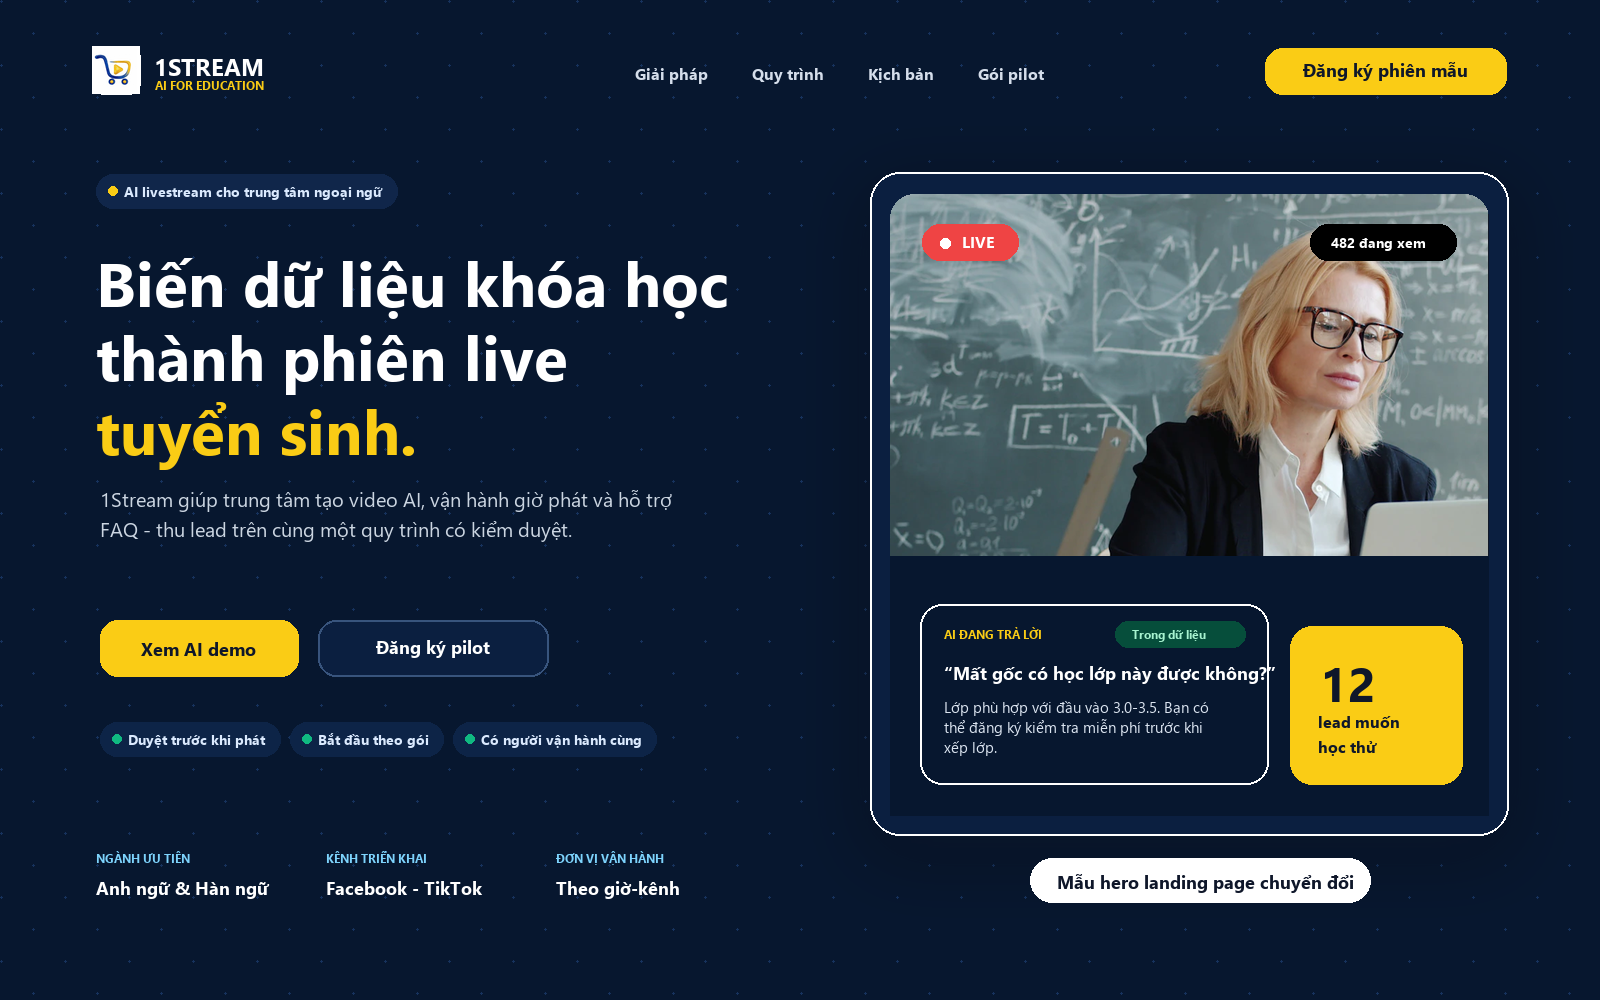
\includegraphics[width=0.95\linewidth]{imgs/PA3_pics/landing_page_hero_mockup.png}
    \caption{Mẫu giao diện hero landing page chuyển đổi của 1Stream}
    \label{fig:pa3_landing_page_hero_mockup}
\end{figure}

\begin{table}[H]
    \centering
    \small
    \setlength{\tabcolsep}{4pt}
    \renewcommand{\arraystretch}{1.22}
    \caption{Các thành phần kỹ thuật tối thiểu của landing page}
    \label{tab:landing-page-components-1stream}
    \rowcolors{2}{paperBg}{white}
    \begin{tabularx}{\linewidth}{@{}L{3.2cm}Y L{3.2cm}@{}}
        \toprule
        \rowcolor{softBlue}
        \textbf{Thành phần} & \textbf{Vai trò chuyển đổi} & \textbf{Sự kiện cần ghi} \\ \midrule

        Tiêu đề và mô tả ngắn &
        Giải thích 1Stream giúp trung tâm tạo/vận hành livestream tuyển sinh từ
        dữ liệu khóa học đã duyệt. &
        \texttt{page\_view} \\

        Video demo ngắn &
        Cho khách thấy ví dụ video AI, cách trả lời câu hỏi và cách thu lead. &
        \texttt{demo\_play}, \texttt{demo\_complete} \\

        Nút đặt lịch demo &
        Chuyển khách có nhu cầu rõ sang bước hẹn tư vấn. &
        \texttt{demo\_cta\_click}, \texttt{booking\_created} \\

        Form đăng ký pilot &
        Thu thông tin để đánh giá mức phù hợp ICP và khả năng chạy thử. &
        \texttt{form\_start}, \texttt{form\_submit} \\

        Checklist dữ liệu cần chuẩn bị &
        Giúp khách biết cần gửi học phí, lịch học, FAQ, ưu đãi và nội dung mẫu
        trước khi pilot. &
        \texttt{checklist\_download} \\

        Thông tin liên hệ Zalo/email &
        Tạo đường dự phòng cho khách chưa muốn điền form hoặc cần hỏi nhanh. &
        \texttt{contact\_click} \\ \bottomrule
    \end{tabularx}
    \rowcolors{2}{}{}
\end{table}

Form thu lead cần ngắn, nhưng đủ dữ liệu để phân biệt lead đại trà và lead phù
hợp ICP. Trong giai đoạn đầu, nhóm có thể dùng Google Form, Tally hoặc một form
đơn giản trên landing page; điều quan trọng là mỗi lượt gửi form phải tự động
đổ về một bảng dữ liệu có thể lọc, chấm điểm và phân công xử lý.

\begin{figure}[H]
    \centering
    
\includegraphics[width=0.95\linewidth]{imgs/PA3_pics/landing_page_form_mockup.png}
    \caption{Mẫu khu vực video demo và form đăng ký pilot trên landing page}
    \label{fig:pa3_landing_page_form_mockup}
\end{figure}

\begin{table}[H]
    \centering
    \footnotesize
    \setlength{\tabcolsep}{3pt}
    \renewcommand{\arraystretch}{1.22}
    \caption{Trường dữ liệu đề xuất trong form đăng ký demo/pilot}
    \label{tab:lead-form-fields-1stream}
    \rowcolors{2}{paperBg}{white}
    \begin{tabularx}{\linewidth}{@{}L{3.0cm}Y L{2.3cm}L{2.4cm}@{}}
        \toprule
        \rowcolor{softBlue}
        \textbf{Trường dữ liệu} &
        \textbf{Mục đích sử dụng} &
        \textbf{Bắt buộc} &
        \textbf{Dùng cho KPI} \\ \midrule

        Tên trung tâm/đơn vị &
        Nhận diện tài khoản khách hàng và tránh trùng lead. &
        Có &
        Lead, ICP \\

        Ngành đào tạo/dịch vụ &
        Kiểm tra có thuộc trung tâm ngoại ngữ hoặc đơn vị bán khóa học hay không. &
        Có &
        Lead phù hợp ICP \\

        Khu vực hoạt động &
        Ưu tiên TP.HCM hoặc khu vực nhóm có thể hỗ trợ trực tiếp. &
        Có &
        ICP, SOM \\

        Người liên hệ và chức vụ &
        Phân biệt chủ trung tâm, trưởng marketing, tư vấn tuyển sinh hoặc nhân
        sự vận hành. &
        Có &
        SQL \\

        Số điện thoại/email/Zalo &
        Dùng để xác nhận demo, chăm sóc sau form và chuyển lead cho người xử lý. &
        Có &
        Tỷ lệ phản hồi \\

        Kênh đang sử dụng &
        Biết khách đang hoạt động trên Facebook, TikTok, YouTube hoặc kênh khác. &
        Có &
        Sẵn sàng kênh \\

        Tần suất livestream &
        Đánh giá cường độ vấn đề và khả năng dùng gói giờ-kênh. &
        Có &
        Lead phù hợp ICP \\

        Dữ liệu khóa học hiện có &
        Xác định khách đã có học phí, lịch học, FAQ, ưu đãi và tài liệu để
        onboarding hay chưa. &
        Có &
        Onboarding \\

        Nhu cầu chính &
        Phân loại khách cần tạo video, vận hành giờ phát, thu lead hoặc gói trọn
        bộ. &
        Có &
        Demo/pilot \\

        Ghi chú hoặc vấn đề đang gặp &
        Thu insight định tính cho sales và product. &
        Không &
        Phản hồi khách hàng \\ \bottomrule
    \end{tabularx}
    \rowcolors{2}{}{}
\end{table}

\subsubsection{Danh sách sự kiện tracking}


\begin{table}[H]
    \centering
    \footnotesize
    \setlength{\tabcolsep}{3pt}
    \renewcommand{\arraystretch}{1.18}
    \caption{Danh sách sự kiện tracking đề xuất cho phễu 1Stream}
    \label{tab:tracking-events-1stream}
    \rowcolors{2}{paperBg}{white}
    \begin{tabularx}{\linewidth}{@{}L{3.2cm}Y Y L{2.4cm}@{}}
        \toprule
        \rowcolor{softBlue}
        \textbf{Event name} &
        \textbf{Khi nào ghi nhận} &
        \textbf{Thông tin đi kèm} &
        \textbf{Nguồn dữ liệu} \\ \midrule

        \texttt{lead\_created} &
        Khi một khách hàng được thêm vào danh sách từ outreach, cộng đồng, đối
        tác hoặc form. &
        Nguồn kênh, tên đơn vị, ngành, khu vực, người phụ trách. &
        CRM/Sheet \\

        \texttt{page\_view} &
        Khi khách truy cập landing page. &
        UTM source, UTM campaign, thiết bị, thời điểm truy cập. &
        Web analytics \\

        \texttt{demo\_play} &
        Khi khách nhấn xem video demo. &
        Vị trí video, nguồn truy cập, thời lượng xem nếu đo được. &
        Web analytics \\

        \texttt{form\_submit} &
        Khi khách gửi form đăng ký demo hoặc pilot. &
        Toàn bộ trường form, nguồn kênh, thời điểm gửi. &
        Form/CRM \\

        \texttt{booking\_created} &
        Khi khách đặt lịch demo thành công. &
        Ngày giờ demo, người phụ trách, trạng thái xác nhận. &
        Calendar/CRM \\

        \texttt{demo\_completed} &
        Khi buổi demo đã diễn ra. &
        Người tham dự, nhu cầu, phản đối chính, mức phù hợp ICP. &
        CRM \\

        \texttt{pilot\_agreed} &
        Khi khách đồng ý chạy thử hoặc gửi dữ liệu mẫu. &
        Gói pilot, phạm vi thử nghiệm, người duyệt nội dung, deadline dữ liệu. &
        CRM \\

        \texttt{onboarding\_completed} &
        Khi khách gửi đủ dữ liệu và nhóm cấu hình xong phiên thử nghiệm. &
        Trạng thái dữ liệu, kênh live, tài khoản, lỗi còn tồn tại. &
        Dashboard/CRM \\

        \texttt{trial\_session\_completed} &
        Khi phiên thử nghiệm đầu tiên hoàn tất. &
        Số giờ-kênh, số bình luận, số lead ghi nhận, trạng thái phát. &
        Dashboard/log phiên \\

        \texttt{feedback\_submitted} &
        Khi khách gửi đánh giá sau demo hoặc sau pilot. &
        Điểm hài lòng, vấn đề, ý định tiếp tục, yêu cầu chỉnh sửa. &
        Survey/CRM \\

        \texttt{paid\_conversion} &
        Khi khách ký hợp đồng hoặc thanh toán gói đầu tiên. &
        Gói mua, giá trị, ngày bắt đầu, nguồn lead, người phụ trách. &
        CRM/bảng doanh thu \\ \bottomrule
    \end{tabularx}
    \rowcolors{2}{}{}
\end{table}

Trong giai đoạn chưa có hệ thống analytics hoàn chỉnh, 1Stream không cần xây
dashboard phức tạp ngay. Nhóm có thể bắt đầu bằng một Google Sheet hoặc Airtable
với các cột cố định, sau đó nhập liệu bán tự động từ form và cập nhật thủ công
các sự kiện như demo, pilot, onboarding hoặc trả phí. Khi số lượng lead tăng,
cấu trúc này có thể được chuyển sang CRM hoặc dashboard nội bộ mà không phải đổi
lại định nghĩa KPI.

\subsubsection{Luồng dữ liệu lead và phân công xử lý}

Luồng dữ liệu lead cần đủ rõ để trả lời câu hỏi: lead đến từ đâu, được lưu ở đâu,
ai chịu trách nhiệm và trạng thái hiện tại là gì. Đối với MVP, luồng dữ liệu đề
xuất như sau:

\begin{center}
\small
\textbf{Kênh quảng bá} $\rightarrow$
\textbf{Landing page / Inbox / Đối tác} $\rightarrow$
\textbf{Form hoặc CRM lead} $\rightarrow$
\textbf{Chấm điểm ICP} $\rightarrow$
\textbf{Người phụ trách demo/pilot} $\rightarrow$
\textbf{Dashboard hoặc báo cáo sau pilot}
\end{center}

\begin{figure}[H]
    \centering
    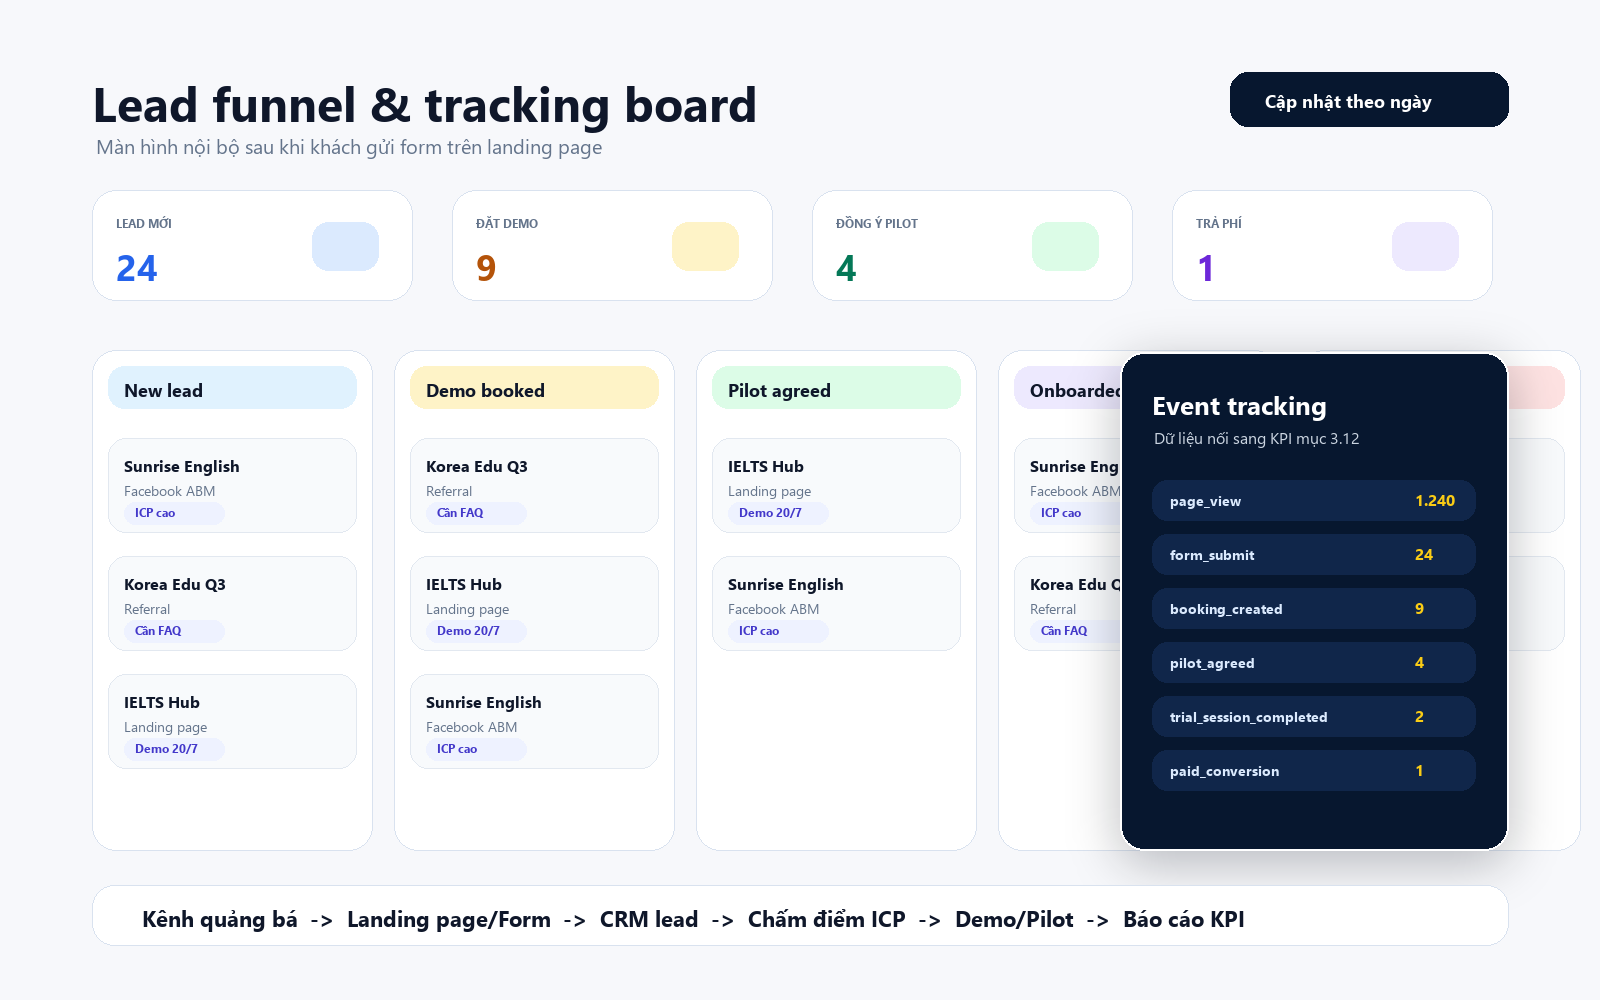
\includegraphics[width=0.95\linewidth]{imgs/PA3_pics/landing_page_tracking_mockup.png}
    \caption{Mẫu bảng theo dõi lead và sự kiện tracking sau khi khách gửi form}
    \label{fig:pa3_landing_page_tracking_mockup}
\end{figure}

\begin{table}[H]
    \centering
    \small
    \setlength{\tabcolsep}{4pt}
    \renewcommand{\arraystretch}{1.22}
    \caption{Nơi lưu dữ liệu và người xử lý theo từng loại lead}
    \label{tab:lead-data-flow-ownership-1stream}
    \rowcolors{2}{paperBg}{white}
    \begin{tabularx}{\linewidth}{@{}L{3.1cm}Y L{3.0cm}L{2.5cm}@{}}
        \toprule
        \rowcolor{softBlue}
        \textbf{Nguồn lead} & \textbf{Cách ghi nhận} & \textbf{Người xử lý chính} & \textbf{Trạng thái cần cập nhật} \\ \midrule

        Tiếp cận trực tiếp/ABM &
        Nhập vào CRM/Sheet ngay khi thêm tài khoản mục tiêu; cập nhật sau mỗi
        lần nhắn tin/gọi điện. &
        Quang + Nhật  &
        New, Contacted, Replied \\

        Landing page/form &
        Tự động ghi vào Sheet/CRM khi khách gửi form; giữ lại UTM/source nếu có. &
        Quang &
        Submitted, Qualified, Demo booked \\

        Workshop/webinar &
        Danh sách đăng ký và danh sách tham dự được nhập vào CRM; gắn tag theo
        tên sự kiện. &
        Quang + Thư&
        Registered, Attended, Follow-up \\

        Đối tác giới thiệu &
        Tạo lead mới kèm tên đối tác giới thiệu và mức độ tin cậy ban đầu. &
        Thư &
        Referral, Demo booked, Pilot proposed \\

        Pilot/sử dụng thử &
        Dữ liệu vận hành lấy từ dashboard hoặc log phiên; kết quả tổng hợp lại
        vào CRM. &
        Nhật + Cảnh &
        Onboarded, Trial completed, Feedback collected \\

        Khách trả phí &
        Ghi nhận gói mua, giá trị, ngày bắt đầu và nguồn lead ban đầu. &
        Toàn + Thư&
        Paid, Retained, Upsell candidate \\ \bottomrule
    \end{tabularx}
    \rowcolors{2}{}{}
\end{table}

Về trách nhiệm kỹ thuật, cần bảo đảm ba điều kiện tối thiểu. Thứ nhất, mọi
lead đều có \textbf{nguồn kênh} để sau này tính hiệu quả từng kênh. Thứ hai, mọi
lead đều có \textbf{trạng thái phễu} để biết đang ở bước nào và ai cần xử lý.
Thứ ba, các sự kiện quan trọng như đặt lịch demo, đồng ý pilot, hoàn tất
onboarding và hoàn tất phiên thử nghiệm phải có \textbf{ngày giờ ghi nhận}, vì
đây là dữ liệu dùng để tính tốc độ chuyển đổi và thời gian từ đăng ký đến phiên
đầu tiên.

\subsubsection{Bảng dữ liệu đo lường cho phễu chuyển đổi}

Các sự kiện tracking cần được định nghĩa thống nhất để nhóm có thể đọc kết quả
phễu theo cùng một cách. Nếu không xác định trước sự kiện và nguồn dữ liệu, các
chỉ số như tỷ lệ đặt lịch demo, tỷ lệ hoàn thành onboarding hoặc CAC sẽ khó tính
nhất quán. Bảng dưới đây tóm tắt dữ liệu cần thu và ý nghĩa của từng nhóm chỉ số.

\begin{table}[H]
    \centering
    \small
    \setlength{\tabcolsep}{4pt}
    \renewcommand{\arraystretch}{1.2}
    \caption{Sự kiện tracking và nhóm chỉ số cần đo trong phễu chuyển đổi}
    \label{tab:tracking-to-kpi-1stream}
    \rowcolors{2}{paperBg}{white}
    \begin{tabularx}{\linewidth}{@{}L{3.4cm}Y Y@{}}
        \toprule
        \rowcolor{softBlue}
        \textbf{Nhóm chỉ số cần đo} & \textbf{Sự kiện/nguồn dữ liệu sử dụng} & \textbf{Ý nghĩa đối với quyết định kênh} \\ \midrule

        Số người tiếp cận &
        \texttt{page\_view}, analytics từ Facebook/TikTok/LinkedIn, danh sách
        outreach. &
        Biết kênh nào tạo được độ phủ ban đầu. \\

        Lượt đăng ký dùng thử/demo &
        \texttt{form\_submit}, \texttt{booking\_created}. &
        Biết kênh nào tạo nhu cầu thật, không chỉ lượt xem. \\

        Tỷ lệ phản hồi từ tiếp cận trực tiếp &
        Số lead trạng thái Replied chia cho số lead Contacted. &
        Đánh giá chất lượng danh sách ABM và thông điệp outreach. \\

        Tỷ lệ demo sang pilot &
        \texttt{demo\_completed}, \texttt{pilot\_agreed}. &
        Biết demo có đủ thuyết phục và khách có đủ điều kiện thử nghiệm không. \\

        Tỷ lệ hoàn thành onboarding &
        \texttt{pilot\_agreed}, \texttt{onboarding\_completed}. &
        Kiểm tra khách có dữ liệu đủ chuẩn và quy trình setup có quá khó không. \\

        Thời gian từ đăng ký đến phiên đầu tiên &
        Thời điểm \texttt{form\_submit} đến \texttt{trial\_session\_completed}. &
        Đánh giá tốc độ triển khai của quy trình kỹ thuật. \\

        Số lead ghi nhận trong pilot &
        Log phiên live, dashboard bình luận/lead, báo cáo sau pilot. &
        Chứng minh giá trị vận hành của 1Stream trong tình huống thật. \\

        Phản hồi và mức hài lòng &
        \texttt{feedback\_submitted}, form khảo sát sau pilot. &
        Xác định điểm cần cải thiện và khả năng chuyển sang trả phí. \\

        Khách hàng trả phí mới &
        \texttt{paid\_conversion}, CRM/bảng doanh thu. &
        Là dữ liệu đầu ra để tính CAC và hiệu quả thương mại. \\ \bottomrule
    \end{tabularx}
    \rowcolors{2}{}{}
\end{table}

Tóm lại, landing page và form giúp thu lead có cấu trúc; danh sách sự kiện giúp
ghi nhận hành vi theo từng bước; CRM/Sheet giúp đội ngũ biết ai đang xử lý lead;
dashboard/log phiên giúp chứng minh giá trị trong pilot. Khi các dữ liệu này
được ghi nhận đều đặn, nhóm có thể đánh giá khách quan kênh nào nên tiếp tục,
kênh nào cần điều chỉnh và kênh nào nên tạm dừng.


% --- PA3-04 | Nguyễn Ngọc Cảnh ---
% ============================================================
% PHẦN 3.9 — KẾ HOẠCH RA MẮT SẢN PHẨM
% ------------------------------------------------------------
% Thuộc: PA3-04
% Người phụ trách chính: Nguyễn Ngọc Cảnh – Operations Lead
% Phối hợp: Nguyễn Anh Thư, Lê Nguyên Nhật
%
% CÂU HỎI CẦN TRẢ LỜI:
%   - Sản phẩm nào thực sự sẵn sàng để giới thiệu ở thời điểm ra mắt?
%   - Nhóm sẽ ra mắt: Prototype? Alpha? Pilot có hỗ trợ? Gói trả phí giới hạn?
%   - Những tính năng nào chưa được phép quảng bá là đã hoàn thiện?
%   - Trước khi ra mắt cần chuẩn bị những tài sản nào?
%   - Ai duyệt nội dung và demo?
%   - Ai tiếp nhận lead?
%   - Ai thực hiện onboarding?
%   - Ai hỗ trợ trong quá trình pilot?
%   - Trước ngày ra mắt cần thực hiện hoạt động gì?
%   - Trong tuần ra mắt cần thực hiện hoạt động gì?
%   - Sau ra mắt cần chăm sóc lead và lấy phản hồi như thế nào?
%   - Khi có lỗi video, dữ liệu hoặc câu trả lời AI thì xử lý ra sao?
%   - Khách hàng phải cung cấp những dữ liệu gì?
%   - Thời gian từ khi đăng ký đến khi chạy được phiên đầu tiên là bao lâu?
%   - Khi nào nhóm dừng một chiến dịch hoặc thay đổi thông điệp?

% OUTPUT BẮT BUỘC:
%   1. Kế hoạch ra mắt theo 3 giai đoạn:
%      - Trước ra mắt
%      - Tuần ra mắt
%      - Sau ra mắt

%   2. Timeline cụ thể:
%      Công việc | Thời gian bắt đầu | Thời gian kết thúc |
%      Người phụ trách | Đầu ra | Điều kiện hoàn thành

%   3. Danh sách tài sản cần chuẩn bị:
%      - Landing page
%      - Video demo
%      - Bộ ảnh hoặc nội dung giới thiệu
%      - Form đăng ký
%      - Kịch bản tư vấn
%      - Bộ câu hỏi thường gặp
%      - Tài liệu onboarding
%      - Phiếu thu phản hồi
%      - Báo cáo sau pilot

%   4. Checklist ra mắt (Chưa làm / Đang làm / Hoàn tất / Bị chặn)

% TIÊU CHÍ HOÀN THÀNH:
%   - Mỗi hoạt động phải tạo ra một đầu ra kiểm tra được
%   - Không viết "đẩy mạnh truyền thông" mà không có hành động cụ thể
%   - Kế hoạch phù hợp với sản phẩm ở giai đoạn PILOT CÓ HỖ TRỢ
%   - Phải xác định người tiếp nhận và xử lý lead
% ============================================================

% TODO (Nguyễn Ngọc Cảnh): Viết nội dung mục 3.9
% Phối hợp Nguyễn Anh Thư để xác nhận timeline phụ thuộc tính năng nào
% Phối hợp Lê Nguyên Nhật để xác nhận tài sản kỹ thuật (landing page, form) sẵn sàng lúc nào


% ============================================================
% PHẦN 3.9 — KẾ HOẠCH RA MẮT SẢN PHẨM
% ============================================================

\subsection{Kế hoạch ra mắt sản phẩm}

Trong giai đoạn đầu, 1Stream không áp dụng chiến lược ``Big Bang Launch" (ra mắt rầm rộ đại chúng) mà chọn cách ra mắt có kiểm soát (Soft Launch) nhắm thẳng vào phân khúc trung tâm ngoại ngữ tại TP.HCM. Mục tiêu cốt lõi là đưa sản phẩm vào môi trường thực chiến để kiểm chứng khả năng vận hành và mức độ sẵn sàng chi trả của khách hàng.

\subsubsection{Định vị sản phẩm tại thời điểm ra mắt và Quy trình hỗ trợ}

\textbf{1. Trạng thái sản phẩm ra mắt}
\begin{itemize}
    \item \textbf{Sản phẩm sẵn sàng ra mắt:} Nhóm triển khai mô hình \textbf{Pilot có hỗ trợ vận hành} (Service-Enabled Software). Cụ thể là Gói thử nghiệm 30 giờ-kênh/tuần. Khách hàng mua kết quả đầu ra (video AI, giờ phát, bot trực FAQ), còn hệ thống phần mềm do đội ngũ 1Stream thao tác nội bộ để đảm bảo chất lượng.
    \item \textbf{Tính năng CHƯA được phép quảng bá:} Tuyệt đối không truyền thông 1Stream là "SaaS tự phục vụ 100\%", không cam kết "phát sóng tự động 24/7 không cần người", không quảng bá tính năng "Tích hợp sâu CRM/ERP", và không hứa hẹn tạo Avatar AI sao chép chính xác 100\% khẩu hình của giáo viên thực tế (chỉ dùng avatar/giọng đọc mẫu có sẵn của hệ thống để tránh rủi ro pháp lý).
\end{itemize}

\textbf{2. Phân công nhân sự vận hành \& Tiếp nhận Lead}
Bám sát cơ cấu tổ chức nhóm (Mục 1.5), quy trình xử lý trong đợt ra mắt được phân công cứng như sau:
\begin{itemize}
    \item \textbf{Tiếp nhận và sàng lọc Lead:} \textbf{Quang (Marketing Lead)} chịu trách nhiệm hứng Lead từ Landing page/Inbox, chấm điểm ICP và chuyển trạng thái MQL sang SQL.
    \item \textbf{Duyệt nội dung \& Trình diễn (Demo):} \textbf{Thư (CEO)} là người trực tiếp thực hiện các buổi Demo B2B với Giám đốc trung tâm và là người chốt quyền duyệt kịch bản cuối cùng trước khi đưa cho khách.
    \item \textbf{Onboarding \& Hỗ trợ dữ liệu:} \textbf{Cảnh (Operations Lead)} chịu trách nhiệm hướng dẫn khách hàng điền form dữ liệu, đốc thúc thu thập tài liệu và chuẩn hóa thành định dạng JSON.
    \item \textbf{Hỗ trợ kỹ thuật Pilot:} \textbf{Nhật (CTO)} chịu trách nhiệm thiết lập luồng phát sóng, kết nối API và giám sát rủi ro server/GPU trong suốt phiên live.
    \item \textbf{Quản lý ngân sách \& Hợp đồng:} \textbf{Toàn (Finance Lead)} quản lý chi phí API/Cloud phát sinh, soạn thảo biên bản thỏa thuận Pilot và chốt hợp đồng trả phí sau khi Pilot kết thúc.
\end{itemize}

\textbf{3. Yêu cầu dữ liệu và Quy trình xử lý sự cố (SLA)}
\begin{itemize}
    \item \textbf{Thời gian triển khai (Time-to-first-run):} Cam kết tối đa \textbf{07 ngày làm việc} kể từ khi khách hàng ký biên bản Pilot đến khi phiên livestream AI đầu tiên được phát sóng.
    \item \textbf{Dữ liệu khách hàng bắt buộc cung cấp:} Bảng giá học phí chuẩn, lịch khai giảng, ưu đãi tháng, 10-15 câu hỏi FAQ thường gặp, yêu cầu đầu vào/đầu ra, và tài liệu xác nhận quyền sở hữu logo/thương hiệu.
    \item \textbf{Quy trình xử lý lỗi (Human-in-the-loop):}
    \begin{itemize}
        \item \textit{Lỗi Video/Hình ảnh:} Nếu Avatar bị lệch khẩu hình hoặc render lỗi, Cảnh (Ops) sẽ tạm dừng lịch phát, Nhật (CTO) render lại bản mới trong vòng 12h.
        \item \textit{Lỗi Dữ liệu/AI trả lời sai:} Hệ thống cài đặt ngưỡng tự tin (confidence score). Nếu AI gặp câu hỏi ngoài Knowledge Base, hệ thống \textbf{tuyệt đối không tự bịa câu trả lời}, mà tự động nhắn: \textit{"Dạ câu hỏi này cần tư vấn chuyên sâu, anh/chị để lại SĐT để giáo vụ bên em gọi lại ngay nhé"}. Đồng thời bắn cảnh báo (ping) về Zalo/Telegram cho nhân viên của trung tâm để vào chat trực tiếp.
    \end{itemize}
\end{itemize}

\subsubsection{Danh sách tài sản cần chuẩn bị trước ra mắt}

Để phục vụ quá trình chuyển đổi, các tài sản (assets) sau phải được nghiệm thu trước Day 1:

\begin{table}[H]
    \centering
    \footnotesize
    \renewcommand{\arraystretch}{1.3}
    \begin{tabularx}{\linewidth}{|l|X|l|}
        \hline
        \rowcolor{softBlue}
        \textbf{Tài sản} & \textbf{Mục đích \& Yêu cầu cốt lõi} & \textbf{Phụ trách} \\ \hline
        \textbf{1. Landing page} & Giao diện trình bày giải pháp hẹp, có nhúng video demo và form thu Lead định danh. & Nhật / Quang \\ \hline
        \textbf{2. Video demo} & Video $\le$ 2 phút quay lại màn hình cách AI của 1Stream lấy dữ liệu Excel và biến thành phiên live. & Quang \\ \hline
        \textbf{3. Nội dung Sales Kit} & Bộ slide Pitch Deck ngắn gọn (5-7 slides) để Thư đi gặp trực tiếp chủ trung tâm. Trọng tâm là bài toán CPL và ROI. & Thư / Toàn \\ \hline
        \textbf{4. Form đăng ký} & Biểu mẫu thu thập: Tên trung tâm, ngân sách Ads hiện tại, số lượng nhân sự trực page (để lọc ICP). & Quang \\ \hline
        \textbf{5. Kịch bản gọi điện} & Kịch bản Telesales (Cold-call) ngắn gọn 3 phút để thiết lập cuộc hẹn Demo. & Quang / Thư \\ \hline
        \textbf{6. Bộ FAQ nội bộ} & Bộ tài liệu xử lý từ chối (Objection Handling) dành cho team Sales khi khách lo sợ rủi ro AI hoặc giá cao. & Thư / Toàn \\ \hline
        \textbf{7. Tài liệu Onboarding} & Template Excel chuẩn hóa để khách hàng điền học phí, lịch học, chính sách bảo lưu một cách dễ nhất. & Cảnh \\ \hline
        \textbf{8. Phiếu thu phản hồi} & Mẫu Google Form (CSAT) dùng sau mỗi phiên live để khách chấm điểm độ thông minh của AI. & Cảnh \\ \hline
        \textbf{9. Báo cáo sau Pilot} & Template báo cáo (PDF) thống kê số giờ tiết kiệm được, số Lead AI thu được để làm bằng chứng Up-sale. & Toàn / Nhật \\ \hline
    \end{tabularx}
\end{table}

\subsubsection{Kế hoạch ra mắt theo 3 giai đoạn}

\textbf{Giai đoạn 1: Trước ra mắt (Pre-launch - Chuẩn bị \& Trinh sát)}
\begin{itemize}
    \item \textbf{Mục tiêu:} Chuẩn bị đạn dược, chốt danh sách mục tiêu và test nội bộ.
    \item \textbf{Hoạt động:} Xây dựng xong Landing Page và 9 tài sản Marketing (mục trên). Quang thực hiện "Trinh sát số" (OSINT) qua Facebook Ads Library để cào danh sách 50-80 trung tâm tiếng Anh tại TP.HCM đang chạy quảng cáo mạnh nhất. Đội Tech tự tạo một trung tâm "ảo", cấp dữ liệu giả để chạy thử toàn bộ luồng từ tạo video đến AI trực chat nhằm bắt bug trước khi mời khách thật.
\end{itemize}

\textbf{Giai đoạn 2: Tuần ra mắt (Launch Week - Tấn công \& Chuyển đổi)}
\begin{itemize}
    \item \textbf{Mục tiêu:} Gặp gỡ trực tiếp và chốt 02-03 trung tâm ký thỏa thuận Pilot.
    \item \textbf{Hoạt động:} Khởi động chiến dịch ABM (Account-Based Marketing). Gửi 50 tin nhắn/email cá nhân hóa đến danh sách đã lọc. Tổ chức 01 buổi Workshop Online nhỏ mời chủ trung tâm vào xem Live Demo. Thư đi gặp trực tiếp (Offline) những khách hàng phản hồi tích cực nhất để chốt cam kết cung cấp dữ liệu Pilot.
\end{itemize}

\textbf{Giai đoạn 3: Sau ra mắt (Post-launch - Vận hành Pilot \& Tối ưu)}
\begin{itemize}
    \item \textbf{Mục tiêu:} Chạy thành công các phiên live bằng dữ liệu thật, thu phản hồi và chuyển đổi thành hợp đồng trả phí.
    \item \textbf{Hoạt động:} Cảnh tiến hành Onboarding, thu thập và làm sạch JSON. Nhật đẩy video lên kênh. Trong 2 tuần Pilot, Cảnh trực nhóm Zalo hỗ trợ khách hàng liên tục. Cuối Pilot, Toàn xuất Báo cáo hiệu suất, Thư họp chốt nghiệm thu và đàm phán ký hợp đồng trả phí (Standard Subscription).
    \item \textbf{Kích hoạt điểm dừng (Pivot/Kill Triggers):} Áp dụng nghiêm ngặt nguyên tắc từ Mục 3.10.4. Nếu tỷ lệ phản hồi tin nhắn tuần ra mắt $< 10\%$, hoặc hết đợt Pilot mà 0 khách hàng nào chịu trả phí, toàn bộ team phải dừng quảng bá, ngồi lại phân tích rào cản giá (Pricing) hoặc độ khó của Onboarding.
\end{itemize}

\subsubsection{Timeline triển khai chi tiết}

\begin{table}[H]
    \centering
    \footnotesize
    \renewcommand{\arraystretch}{1.4}
    \begin{tabularx}{\linewidth}{|p{3.5cm}|c|c|c|X|X|}
        \hline
        \rowcolor{softBlue}
        \textbf{Công việc} & \textbf{Bắt đầu} & \textbf{Kết thúc} & \textbf{Phụ trách} & \textbf{Đầu ra (Output)} & \textbf{Điều kiện hoàn thành} \\ \hline
        
        1. Xây dựng Landing Page \& Video Demo & Ngày 1 & Ngày 7 & Nhật, Quang & Landing page live (URL), 1 Video Demo & Form đăng ký hoạt động, luồng lead đổ về Sheet/CRM. \\ \hline
        
        2. Quét \& Chấm điểm danh sách ABM (50-80 Leads) & Ngày 5 & Ngày 10 & Quang & Danh sách Lead chuẩn ICP (Google Sheet) & 100\% Lead có tên GĐ/Trưởng phòng, có chạy Ads. \\ \hline
        
        3. Tạo Template Onboarding \& Kịch bản Sales & Ngày 8 & Ngày 12 & Thư, Cảnh & Bộ tài liệu Sales Kit, Template Excel & Thư duyệt kịch bản, Cảnh test thử việc điền form. \\ \hline
        
        4. Test nội bộ toàn hệ thống (Alpha Test) & Ngày 10 & Ngày 14 & Nhật, Cảnh & Bảng report Bug \& Tối ưu & Chạy mượt 1 phiên live 30p, bot AI phản hồi $\le$ 3s. \\ \hline
        
        5. Tổ chức Workshop Demo Online & Ngày 15 & Ngày 18 & Thư, Quang & 1 buổi Zoom, Record video, 3-5 booking & Có ít nhất 15 người tham dự đúng ngành. \\ \hline
        
        6. Triển khai Outreach trực tiếp \& Đặt lịch hẹn & Ngày 16 & Ngày 21 & Quang, Thư & 5-8 lịch hẹn Demo 1-1 (Discovery Call) & Tỷ lệ phản hồi tin nhắn/email $\ge$ 20\%. \\ \hline
        
        7. Gặp mặt, Chốt cam kết Pilot & Ngày 20 & Ngày 25 & Thư, Toàn & 02-03 Biên bản đồng ý Pilot & Khách cam kết cử người phối hợp làm dữ liệu. \\ \hline
        
        8. Onboarding, Xử lý dữ liệu \& Chạy phiên Pilot & Ngày 26 & Ngày 40 & Cảnh, Nhật & Các phiên Live chạy thực tế trên kênh & Hoàn thành đủ số giờ Pilot đã cam kết, hệ thống ổn định. \\ \hline
        
        9. Đánh giá CSAT \& Chốt hợp đồng trả phí & Ngày 40 & Ngày 45 & Thư, Toàn & Báo cáo hiệu suất, 1-2 Hợp đồng trả phí & Khách đồng ý ký HĐ trả tiền mặt cho tháng tiếp theo. \\ \hline
    \end{tabularx}
\end{table}

\subsubsection{Checklist sẵn sàng ra mắt (Launch Readiness Checklist)}

\begin{table}[H]
    \centering
    \footnotesize
    \renewcommand{\arraystretch}{1.3}
    \begin{tabularx}{\linewidth}{|l|c|X|}
        \hline
        \rowcolor{softBlue}
        \textbf{Hạng mục kiểm tra} & \textbf{Trạng thái} & \textbf{Ghi chú / Người xử lý} \\ \hline
        Hoàn thiện Backend sinh Video AI \& RAG AI Agent & Đang làm & Nhật đang tối ưu tốc độ phản hồi (Latency). \\ \hline
        Hoàn thiện Landing Page \& Hệ thống Tracking (Mục 3.8) & Đang làm & Nhật \& Quang setup UTM tracking. \\ \hline
        Xây dựng xong danh sách 80 khách hàng mục tiêu & Chưa làm & Quang chờ kịch bản lọc ICP cuối cùng. \\ \hline
        Thiết kế Bảng giá (Pricing) dự kiến & Hoàn tất & Toàn đã chốt 3 kịch bản giá Pilot. \\ \hline
        Tài liệu Template Onboarding cho khách hàng & Hoàn tất & Cảnh đã đóng gói file Excel mẫu. \\ \hline
        Kịch bản thuyết phục \& Xử lý từ chối (Sales Script) & Đang làm & Thư đang hoàn thiện bộ FAQ cho Sales. \\ \hline
        Quy trình xử lý sự cố (SLA) khi Video/Live bị sập & Hoàn tất & Nhóm đã thống nhất luồng hỗ trợ thủ công. \\ \hline
        Hợp đồng mẫu / Biên bản thỏa thuận bảo mật dữ liệu & Bị chặn & Chờ cố vấn pháp lý duyệt điều khoản bản quyền AI. \\ \hline
    \end{tabularx}
\end{table}

% --- PA3-04 | Nguyễn Ngọc Cảnh ---
% ============================================================
% PHẦN 3.10 — HOẠT ĐỘNG MARKETING TRONG GIAI ĐOẠN ĐẦU
% ------------------------------------------------------------
% Thuộc: PA3-04
% Người phụ trách chính: Nguyễn Ngọc Cảnh – Operations Lead
% Phối hợp: Nguyễn Anh Thư, Lê Nguyên Nhật
%
% CÂU HỎI CẦN TRẢ LỜI:
%   - Trước ngày ra mắt cần thực hiện hoạt động gì?
%   - Trong tuần ra mắt cần thực hiện hoạt động gì?
%   - Sau ra mắt cần chăm sóc lead và lấy phản hồi như thế nào?
%   - Khi nào nhóm dừng một chiến dịch hoặc thay đổi thông điệp?

% OUTPUT BẮT BUỘC:
%   1. Lịch hoạt động marketing giai đoạn đầu:
%      - Bài giới thiệu vấn đề
%      - Video demo
%      - Tình huống sử dụng (use case)
%      - Workshop
%      - Tiếp cận trực tiếp (outreach)
%      - Mời pilot
%      - Nội dung phản hồi hoặc case study

%   2. Quy trình vận hành pilot:
%      Sàng lọc khách hàng
%        → Tiếp nhận dữ liệu
%        → Chuẩn hóa dữ liệu
%        → Tạo nội dung
%        → Duyệt
%        → Chạy thử
%        → Ghi nhận số liệu
%        → Phỏng vấn sau thử nghiệm
%        → Đề xuất trả phí

% TIÊU CHÍ HOÀN THÀNH:
%   - Không viết "tăng nhận diện" mà không có hành động cụ thể
%   - Mỗi hoạt động phải tạo ra một đầu ra kiểm tra được
%   - Kế hoạch phù hợp với giai đoạn pilot có hỗ trợ, chưa phải SaaS tự phục vụ
% ============================================================

% TODO (Nguyễn Ngọc Cảnh): Viết nội dung mục 3.10
% Lấy kênh đã được chốt từ 3.6 và thông điệp từ 3.5 để tạo lịch nội dung cụ thể


% ============================================================
% PHẦN 3.10 — HOẠT ĐỘNG MARKETING TRONG GIAI ĐOẠN ĐẦU
% ============================================================

\subsection{Hoạt động marketing trong giai đoạn đầu}

Trong giai đoạn đầu (MVP), mục tiêu của hoạt động marketing không phải là phủ sóng diện rộng, mà là tìm kiếm, giáo dục và thuyết phục thành công nhóm khách hàng tiên phong (các trung tâm ngoại ngữ tại TP.HCM quy mô 3-5 nhân sự) tham gia chạy thử nghiệm (Pilot). Các hoạt động được thiết kế gắn liền với đầu ra có thể đo lường được.

\subsubsection{Lịch hoạt động marketing giai đoạn đầu}

\textbf{A. Trước ngày ra mắt (Tuần 1 - Tuần 2: Tạo mồi nhử và vật liệu truyền thông)}
\begin{itemize}
    \item \textbf{Bài giới thiệu vấn đề:} Đăng tải các bài phân tích ngắn trên các cộng đồng quản lý giáo dục/chủ trung tâm ngoại ngữ. Nội dung xoáy thẳng vào nỗi đau: ``Sự lãng phí chi phí nhân sự trực ca đêm và rủi ro rớt lead khi chạy Ads tuyển sinh".
    \begin{itemize}
        \item \textit{Đầu ra kiểm tra được:} 02 bài post trên hội nhóm, đạt tối thiểu 15 bình luận thảo luận từ đúng đối tượng ICP.
    \end{itemize}
    \item \textbf{Video demo:} Quay màn hình thực tế (screen-recording) thể hiện luồng làm việc của 1Stream: từ một bảng giá học phí Excel $\rightarrow$ Video AI giới thiệu khóa học $\rightarrow$ AI Sales Agent tự động trả lời bình luận hỏi giá. Đăng tải lên Landing page và kênh Facebook/TikTok của dự án.
    \begin{itemize}
        \item \textit{Đầu ra kiểm tra được:} 01 Video demo hoàn chỉnh (dưới 2 phút) được nhúng thành công lên Landing page.
    \end{itemize}
    \item \textbf{Tình huống sử dụng (Use case):} Đóng gói một tài liệu ngắn mô phỏng cách một trung tâm tiếng Anh nhỏ dùng 1Stream để treo livestream 30 giờ/tuần mà không cần thuê thêm host.
    \begin{itemize}
        \item \textit{Đầu ra kiểm tra được:} 01 file PDF "Sổ tay tối ưu chi phí livestream tuyển sinh" dùng làm Lead Magnet (quà tặng đổi lấy email/Zalo của khách hàng).
    \end{itemize}
\end{itemize}

\textbf{B. Trong tuần ra mắt (Tuần 3: Tiếp cận và chuyển đổi)}
\begin{itemize}
    \item \textbf{Workshop chuyên đề (Kênh phễu giữa):} Tổ chức một buổi chia sẻ trực tuyến (Zoom/Google Meet) với chủ đề "Tối ưu chi phí livestream và chống rò rỉ Lead ca tối". Thực hiện demo sản phẩm trực tiếp (Live Demo) ngay trong buổi này.
    \begin{itemize}
        \item \textit{Đầu ra kiểm tra được:} Tổ chức thành công 01 buổi workshop, thu hút 15-20 người tham gia thực tế, thu về ít nhất 3 yêu cầu dùng thử.
    \end{itemize}
    \item \textbf{Tiếp cận trực tiếp (Outreach - ABM):} Triển khai kịch bản nhắn tin/gọi điện trực tiếp (Cold Outreach) qua LinkedIn, Zalo hoặc Email tới danh sách 50-80 tài khoản khách hàng mục tiêu đã chấm điểm ICP.
    \begin{itemize}
        \item \textit{Đầu ra kiểm tra được:} Gửi thành công 50 tin nhắn tiếp cận, xác nhận được 5-8 lịch hẹn gọi Demo (Discovery Call) 1-1.
    \end{itemize}
    \item \textbf{Mời pilot:} Đưa ra lời kêu gọi hành động (CTA) rõ ràng cuối buổi Demo/Workshop: Mời khách hàng trải nghiệm gói vận hành 30 giờ-kênh/tuần với chi phí ưu đãi (hoặc đặt cọc cam kết).
    \begin{itemize}
        \item \textit{Đầu ra kiểm tra được:} 02 đến 03 khách hàng ký biên bản đồng ý tham gia Pilot và bàn giao người đầu mối làm việc.
    \end{itemize}
\end{itemize}

\textbf{C. Sau ra mắt (Tuần 4 trở đi: Chăm sóc và Chứng minh giá trị)}
\begin{itemize}
    \item \textbf{Nội dung phản hồi hoặc Case study:} Sau khi phiên pilot đầu tiên kết thúc, tổng hợp số liệu thực tế (số giờ tiết kiệm được, số câu hỏi AI trả lời đúng, số lead thu về) thành một bài học thành công (Case study).
    \begin{itemize}
        \item \textit{Đầu ra kiểm tra được:} 01 bài báo cáo Case Study (ẩn danh hoặc công khai tên trung tâm nếu được cho phép) gửi lại cho toàn bộ danh sách khách hàng đang ở trạng thái "Đang cân nhắc" (Nurturing).
    \end{itemize}
\end{itemize}

\subsubsection{Quy trình vận hành pilot (Mô hình Service-Enabled Software)}

Vì sản phẩm ở giai đoạn này chưa phải là SaaS tự phục vụ hoàn toàn, quy trình Pilot được thiết kế để đội ngũ 1Stream trực tiếp hỗ trợ, giúp giảm rủi ro lỗi kỹ thuật và giảm "chi phí học hỏi" cho khách hàng.

\begin{enumerate}
    \item \textbf{Sàng lọc khách hàng:} Đối chiếu thông tin khách hàng đăng ký với Ma trận chấm điểm ICP (Mục 3.3). Chỉ duyệt các trung tâm đạt >75 điểm (có đủ dữ liệu tĩnh, có nhân sự phối hợp, đúng ngành).
    \begin{itemize}
        \item \textit{Đầu ra:} Bảng chấm điểm duyệt điều kiện tham gia Pilot.
    \end{itemize}
    \item \textbf{Tiếp nhận dữ liệu:} Khách hàng điền thông tin vào "Biểu mẫu Onboarding" do 1Stream cung cấp, bao gồm: bảng học phí, lịch khai giảng, ưu đãi, FAQ và kịch bản tư vấn chuẩn.
    \begin{itemize}
        \item \textit{Đầu ra:} Thư mục lưu trữ dữ liệu thô của khách hàng.
    \end{itemize}
    \item \textbf{Chuẩn hóa dữ liệu:} Đội ngũ Vận hành (Operations) của 1Stream rà soát, làm sạch và chuyển đổi dữ liệu thô thành định dạng Knowledge Base (JSON) để AI có thể hiểu và truy xuất chính xác.
    \begin{itemize}
        \item \textit{Đầu ra:} Bộ cơ sở tri thức (Knowledge Base) đã được chuẩn hóa.
    \end{itemize}
    \item \textbf{Tạo nội dung:} Dùng hệ thống 1Stream để sinh kịch bản livestream, khởi tạo giọng đọc/Avatar AI và ghép video, thêm phụ đề dựa trên dữ liệu đã chuẩn hóa.
    \begin{itemize}
        \item \textit{Đầu ra:} Bản nháp Video AI và Kịch bản chữ.
    \end{itemize}
    \item \textbf{Duyệt:} Gửi bản nháp cho Người duyệt nội dung của trung tâm kiểm tra. Giới hạn chỉnh sửa tối đa 2 lần để đảm bảo tiến độ.
    \begin{itemize}
        \item \textit{Đầu ra:} Email/Tin nhắn xác nhận "Approve" (Đồng ý phát sóng) từ khách hàng.
    \end{itemize}
    \item \textbf{Chạy thử:} Đội ngũ 1Stream thiết lập luồng phát sóng, kết nối API lên kênh Facebook/TikTok của khách hàng và giám sát trạng thái hệ thống trong suốt thời gian diễn ra phiên live.
    \begin{itemize}
        \item \textit{Đầu ra:} Phiên livestream diễn ra thành công trên kênh của khách hàng, không bị gián đoạn tín hiệu.
    \end{itemize}
    \item \textbf{Ghi nhận số liệu:} Xuất nhật ký (log) của hệ thống: Thời lượng phát sóng thực tế, tổng số bình luận, số câu AI trả lời đúng, số trường hợp phải chuyển cho nhân viên thật, số Lead thu được.
    \begin{itemize}
        \item \textit{Đầu ra:} Báo cáo hiệu suất phiên Livestream (Session Report).
    \end{itemize}
    \item \textbf{Phỏng vấn sau thử nghiệm:} Đặt lịch gọi 15 phút với chủ trung tâm hoặc nhân viên trực page để đánh giá độ hài lòng: AI trả lời có tự nhiên không? Áp lực công việc có giảm không?
    \begin{itemize}
        \item \textit{Đầu ra:} Biên bản phỏng vấn / Khảo sát CSAT.
    \end{itemize}
    \item \textbf{Đề xuất trả phí:} Dựa trên báo cáo hiệu suất và phản hồi tích cực, đội ngũ Sales gửi hợp đồng đề xuất chuyển đổi sang Gói dịch vụ trả phí (Starter/Standard).
    \begin{itemize}
        \item \textit{Đầu ra:} Hợp đồng được ký kết, hoặc lý do từ chối rõ ràng được ghi nhận vào CRM.
    \end{itemize}
\end{enumerate}

\subsubsection{Chăm sóc Lead và thu thập phản hồi}

\begin{itemize}
    \item \textbf{Chăm sóc Lead (Lead Nurturing):} Các khách hàng rớt ở khâu "Sàng lọc" (do chưa sẵn sàng dữ liệu) sẽ được đưa vào chuỗi chăm sóc tự động qua Email/Zalo. Nhóm sẽ gửi tặng họ "Bộ Template Excel chuẩn hóa dữ liệu tuyển sinh" để họ tự hoàn thiện nội bộ, tạo tiền đề tiếp cận lại vào tháng sau.
    \item \textbf{Thu thập phản hồi (Feedback Loop):} Áp dụng nguyên tắc phản hồi nhanh gọn (micro-feedback). Thay vì gửi các form khảo sát dài, nhóm vận hành sẽ tương tác trực tiếp qua Zalo group chung với khách hàng ngay sau mỗi ca live: \textit{"Hôm nay AI nhận diện 12 lead hỏi học phí lớp IELTS, bên mình đánh giá câu trả lời đã đúng giọng điệu trung tâm chưa ạ?"}. Mọi góp ý (dù là phàn nàn) đều được ghi nhận vào Ticket hệ thống để CTO điều chỉnh prompt ngay lập tức.
\end{itemize}

\subsubsection{Tiêu chí dừng chiến dịch hoặc thay đổi thông điệp (Pivot/Kill Triggers)}

Để bảo vệ nguồn lực giới hạn, nhóm marketing sẽ liên tục đo lường dựa trên bộ KPI (Mục 3.12) và áp dụng kỷ luật thép để dừng/đổi chiến dịch nếu vi phạm các ngưỡng sau:

\begin{enumerate}
    \item \textbf{Thông điệp không chạm đúng Nỗi đau:} Nếu chiến dịch "Tiếp cận trực tiếp" (Outreach) gửi đi 50 tin nhắn cho các đối tượng đã lọc kỹ (Core ICP) mà \textbf{tỷ lệ phản hồi (Reply rate) dưới 10\%} sau 1 tuần $\rightarrow$ Cần lập tức dừng gửi. Đổi thông điệp từ việc "Nói về tính năng tạo video AI" sang "Đánh thẳng vào số tiền lương ngoài giờ họ đang lãng phí mỗi tháng".
    \item \textbf{Rào cản quy trình quá lớn:} Nếu khách hàng đồng ý xem Demo (tỷ lệ đặt lịch cao) nhưng ở bước \textbf{"Tiếp nhận dữ liệu" có tỷ lệ rớt (Drop-off) lớn hơn 50\%} (khách hàng phàn nàn việc chuẩn bị dữ liệu quá mệt mỏi) $\rightarrow$ Dừng việc bán gói Pilot hiện tại. Hệ thống phải đổi chiến thuật: Thiết kế sẵn các gói Template kịch bản mẫu cho ngành tiếng Anh để khách chỉ cần điền giá tiền, thay vì bắt khách tự viết từ số không.
    \item \textbf{Chi phí thu Lead (CPL) mất kiểm soát:} Nếu sử dụng ngân sách cho các hoạt động đẩy hội thảo (Workshop) nhưng tính toán lại \textbf{CPL cao hơn 2 lần mức cho phép} hoặc tập khách hàng thu về toàn là cá nhân bán hàng nhỏ lẻ không có ngân sách (Sai ICP) $\rightarrow$ Dừng kênh Workshop đại trà, quay lại chiến dịch "Bắn tỉa" (ABM) từng trung tâm cụ thể.
    \item \textbf{Tỷ lệ Chuyển đổi Trả phí bằng 0:} Nếu hoàn tất 3 đợt Pilot thành công, AI hoạt động tốt, khách hàng khen ngợi nhưng \textbf{không có ai đồng ý đề xuất trả phí} $\rightarrow$ Dừng ngay các chiến dịch Marketing mở rộng phễu. Vấn đề nằm ở Cấu trúc Giá (Pricing) hoặc ROI khách hàng nhận được chưa đủ bù đắp chi phí thuê 1Stream. Phải ngồi lại với 3 khách hàng Pilot để tái cấu trúc gói sản phẩm trước khi tìm khách mới.
\end{enumerate}

% --- PA3-05 | Nguyễn Công Toàn ---
% ============================================================
% PHẦN 3.11 — NGÂN SÁCH VÀ NGUỒN LỰC QUẢNG BÁ
% ------------------------------------------------------------
% Thuộc: PA3-05
% Người phụ trách chính: Nguyễn Công Toàn – Finance Lead
% Phối hợp dữ liệu: Lê Nguyên Nhật
%
% CÂU HỎI CẦN TRẢ LỜI:
%   - Tổng ngân sách quảng bá thử nghiệm là bao nhiêu?
%   - Nhóm có thể chi bao nhiêu tiền để tìm một lead?
%   - Chi phí nào là chi phí tiền mặt? Chi phí nào là thời gian của thành viên?
%   - Kênh nào có chi phí cố định? Kênh nào có chi phí theo mỗi lượt tiếp cận/lead?
%   - Công thức tính CAC là gì?
%   - Khi chưa có khách hàng trả phí, có thể tính CAC dự kiến như thế nào?
%
% OUTPUT BẮT BUỘC:
%   1. Bảng ngân sách theo kênh:
%      Kênh | Hoạt động | Chi phí dự kiến | Nhân lực |
%      Thời gian thực hiện | Kết quả kỳ vọng | Giới hạn chi tiêu
%
%   2. Ba kịch bản ngân sách:
%      - Tối thiểu
%      - Cơ sở
%      - Mở rộng
%
%   Lưu ý:
%     CAC = Tổng chi phí bán hàng và quảng bá / Số khách hàng trả phí mới
%     (Khi chưa có dữ liệu thật → ghi là "mục tiêu thử nghiệm" hoặc "giả định ban đầu")
%
% TIÊU CHÍ HOÀN THÀNH:
%   - Khi chưa có dữ liệu thật, phải ghi là GIẢ ĐỊNH BAN ĐẦU
%   - Phân biệt lead / lead phù hợp ICP / người đăng ký demo /
%     người dùng thử / khách hàng trả phí
% ============================================================

\subsection{Ngân sách và nguồn lực quảng bá}

% ============================================================
% GHI CHÚ TRẠNG THÁI (19/07/2026):
%   Đây là KHUNG mục 3.11. Các con số ngân sách phụ thuộc vào danh sách kênh
%   (3.6), kế hoạch ra mắt (3.9) và hoạt động marketing (3.10) — cả ba hiện
%   CHƯA được chốt. Vì vậy các giá trị tiền mặt, số giờ và giới hạn chi tiêu
%   được đánh dấu bằng \placeholder{...} để điền sau khi ba mục trên hoàn tất.
%   Phần định tính (phân loại chi phí, vai trò kênh, điều kiện kịch bản) đã điền
%   sẵn vì không phụ thuộc số liệu. Danh sách kênh dưới đây bám theo các kênh ví
%   dụ nêu ở 3.6 và cần được thay bằng danh sách kênh chính thức khi 3.6 chốt.
% ============================================================

Ngân sách quảng bá của 1Stream được lập cho giai đoạn Pilot kéo dài khoảng ba tháng, dưới ràng buộc nguồn lực của một nhóm khởi nghiệp sinh viên: dòng tiền mặt hạn chế và nhân lực kiêm nhiệm. Do đó, nguyên tắc xuyên suốt là ưu tiên các kênh có chi phí tiền mặt thấp và tận dụng chi phí thời gian của thành viên, chỉ chi tiền mặt cho những hạng mục có khả năng đo lường rõ ràng và có thể dừng nhanh khi không hiệu quả.

Bảng ngân sách trong mục này được xây dựng \emph{dựa trên} các hoạt động và kênh quảng bá được chốt ở mục 3.6 (lựa chọn kênh), 3.9 (kế hoạch ra mắt) và 3.10 (hoạt động marketing). Tại thời điểm soạn khung này, ba mục trên chưa hoàn tất, nên các con số tiền mặt, số giờ nhân lực và hạn mức chi tiêu được để ở dạng \placeholder{giá trị cần điền} và sẽ được cập nhật ngay khi danh sách kênh chính thức được xác nhận. Việc lập ngân sách chỉ được coi là hoàn chỉnh sau khi ICP, thông điệp và kênh đã chốt --- đây là điều kiện tiên quyết đã thống nhất trong nhóm.

\subsubsection{Phân loại chi phí quảng bá}

Trước khi lập bảng, nhóm phân biệt rõ hai cặp loại chi phí để tránh nhầm lẫn giữa tiền thực chi và công sức bỏ ra, cũng như giữa chi phí không đổi và chi phí tăng theo quy mô. Cách phân loại này quyết định cột ``Chi phí dự kiến'' và ``Giới hạn chi tiêu'' trong bảng ngân sách.

\begin{table}[H]
    \centering
    \footnotesize
    \setlength{\tabcolsep}{4pt}
    \renewcommand{\arraystretch}{1.3}
    \caption{Phân loại chi phí quảng bá áp dụng cho 1Stream}
    \label{tab:pa3-ns-phanloai}
    \begin{tabularx}{\linewidth}{@{}L{0.22\linewidth} L{0.34\linewidth} Y@{}}
        \toprule
        \rowcolor{softBlue}
        \textbf{Loại chi phí} & \textbf{Định nghĩa} & \textbf{Ví dụ trong 1Stream} \\ \midrule
        \textbf{Chi phí tiền mặt} & Khoản tiền thực sự chi ra khỏi ngân sách. & Quảng cáo trả phí trên Facebook/TikTok, tên miền và hosting cho landing page, công cụ gửi email. \\
        \textbf{Chi phí thời gian} & Thời gian và công sức của thành viên; không xuất tiền mặt nhưng có chi phí cơ hội. & Gọi và nhắn tin tiếp cận trực tiếp, sản xuất video, trực và vận hành phiên livestream. \\
        \textbf{Chi phí cố định} & Không thay đổi theo số lead hay lượt tiếp cận. & Tên miền, hosting, chi phí thiết lập landing page ban đầu. \\
        \textbf{Chi phí biến đổi} & Tăng theo mỗi lượt tiếp cận hoặc mỗi lead. & Chi phí quảng cáo tính theo lượt nhấp, chi phí tổ chức mỗi buổi workshop. \\
        \bottomrule
    \end{tabularx}
\end{table}

\subsubsection{Bảng ngân sách theo kênh}

Bảng dưới đây liệt kê các kênh dự kiến (bám theo các kênh ví dụ ở mục 3.6) cùng hoạt động, chi phí, nhân lực, thời gian và kết quả kỳ vọng. Cột ``Kết quả kỳ vọng'' được liên kết trực tiếp với các KPI ở mục 3.12 để mỗi đồng chi ra đều gắn với một chỉ số đo được. Các ô \placeholder{...} chờ số liệu sau khi mục 3.6, 3.9 và 3.10 chốt.

\begingroup
\scriptsize
\setlength{\tabcolsep}{2pt}
\renewcommand{\arraystretch}{1.3}
\begin{longtable}{@{}
    >{\raggedright\arraybackslash}p{2.2cm}
    >{\raggedright\arraybackslash}p{2.9cm}
    >{\raggedright\arraybackslash}p{2.6cm}
    >{\raggedright\arraybackslash}p{2.2cm}
    >{\raggedright\arraybackslash}p{1.5cm}
    >{\raggedright\arraybackslash}p{2.5cm}
    >{\raggedright\arraybackslash}p{1.4cm}@{}}
\caption{Khung ngân sách quảng bá theo kênh giai đoạn Pilot (số liệu chờ chốt từ 3.6, 3.9, 3.10)}
\label{tab:pa3-ns-kenh}\\
\toprule
\rowcolor{softBlue}
\textbf{Kênh} & \textbf{Hoạt động chính} & \textbf{Chi phí dự kiến} & \textbf{Nhân lực (thời gian)} & \textbf{Thời gian} & \textbf{Kết quả kỳ vọng} & \textbf{Giới hạn chi tiêu} \\
\midrule
\endfirsthead
\multicolumn{7}{@{}l}{\footnotesize\itshape (tiếp theo Bảng~\ref{tab:pa3-ns-kenh})}\\
\toprule
\rowcolor{softBlue}
\textbf{Kênh} & \textbf{Hoạt động chính} & \textbf{Chi phí dự kiến} & \textbf{Nhân lực (thời gian)} & \textbf{Thời gian} & \textbf{Kết quả kỳ vọng} & \textbf{Giới hạn chi tiêu} \\
\midrule
\endhead
\midrule
\multicolumn{7}{@{}r@{}}{\footnotesize\itshape Còn tiếp \dots}\\
\endfoot
\bottomrule
\endlastfoot

Tiếp cận trực tiếp (direct outreach) & Gọi điện, email và nhắn tin đến trung tâm ICP; giới thiệu và mời demo & Tiền mặt gần bằng 0; chủ yếu là chi phí thời gian & Thư, Quang --- \placeholder{số giờ/tuần} & Suốt pilot & 40--60 trung tâm tiếp cận; 20--30\% phản hồi (mục 3.12) & \placeholder{hạn mức} \\
Cộng đồng giáo dục (Facebook Group, hội nhóm chủ trung tâm) & Đăng bài chia sẻ, tư vấn, xây uy tín và thu lead & Tiền mặt gần bằng 0; chi phí thời gian & Quang --- \placeholder{số giờ/tuần} & Suốt pilot & Góp vào chỉ tiêu lead ghi nhận và lead phù hợp ICP & \placeholder{hạn mức} \\
Nội dung TikTok/Facebook & Sản xuất video minh họa tình huống dùng sản phẩm (tạo bằng chính 1Stream) & Tiền mặt: \placeholder{VND} nếu chạy quảng cáo; còn lại là thời gian & Nhật, Quang --- \placeholder{số giờ/tuần} & Suốt pilot & Số người tiếp cận và lượt tương tác (mục 3.12) & \placeholder{hạn mức ads} \\
Workshop/webinar trực tuyến & Tổ chức buổi demo giải pháp cho nhóm trung tâm quan tâm & Tiền mặt: \placeholder{VND} (công cụ họp, có thể dùng bản miễn phí) & Thư --- \placeholder{số giờ/buổi} & \placeholder{số buổi} trong pilot & Số lịch demo và số đơn vị đồng ý pilot & \placeholder{hạn mức/buổi} \\
Landing page và biểu mẫu & Trang thu thông tin, đặt lịch demo và đăng ký dùng thử & Tiền mặt: \placeholder{VND} (tên miền, hosting) --- chi phí cố định & Nhật --- \placeholder{số giờ thiết lập} & Thiết lập đầu pilot & Nơi ghi nhận lead và điểm khởi đầu của phễu (mục 3.8) & \placeholder{hạn mức} \\
Email chăm sóc & Gửi thông tin và nuôi dưỡng lead sau tiếp xúc đầu tiên & Tiền mặt: \placeholder{VND} (công cụ email) & Quang --- \placeholder{số giờ/tuần} & Suốt pilot & Tăng tỷ lệ đặt demo từ lead đã có & \placeholder{hạn mức} \\
\end{longtable}
\endgroup

{\footnotesize\itshape Danh sách kênh trên là dự kiến theo mục 3.6; cần thay bằng danh sách kênh chính thức và điền số liệu sau khi 3.6, 3.9 và 3.10 được chốt.}

\subsubsection{Ba kịch bản ngân sách}

Nhóm chuẩn bị ba kịch bản để chủ động theo mức nguồn lực thực tế. Ba kịch bản dùng chung khung kênh ở Bảng~\ref{tab:pa3-ns-kenh} nhưng khác nhau ở mức chi tiền mặt và số kênh trả phí được kích hoạt. Các cột định tính (kênh sử dụng và điều kiện áp dụng) đã được xác định; các con số chờ chốt cùng với bảng ngân sách.

\begin{table}[H]
    \centering
    \footnotesize
    \setlength{\tabcolsep}{4pt}
    \renewcommand{\arraystretch}{1.3}
    \caption{Ba kịch bản ngân sách quảng bá giai đoạn Pilot}
    \label{tab:pa3-ns-kichban}
    \begin{tabularx}{\linewidth}{@{}L{0.20\linewidth} Y Y Y@{}}
        \toprule
        \rowcolor{softBlue}
        \textbf{Chỉ tiêu} & \textbf{Tối thiểu} & \textbf{Cơ sở} & \textbf{Mở rộng} \\ \midrule
        \textbf{Tổng ngân sách tiền mặt (3 tháng)} & \placeholder{VND} & \placeholder{VND} & \placeholder{VND} \\
        \textbf{Kênh sử dụng} & Chỉ kênh không tốn tiền mặt: tiếp cận trực tiếp, cộng đồng, nội dung tự nhiên & Thêm workshop và landing page có chi phí cố định thấp & Thêm quảng cáo trả phí có kiểm soát trên TikTok/Facebook \\
        \textbf{Số lead kỳ vọng} & \placeholder{số lead} & \placeholder{số lead} & \placeholder{số lead} \\
        \textbf{Số pilot kỳ vọng} & \placeholder{số pilot} & \placeholder{số pilot} & \placeholder{số pilot} \\
        \textbf{Số khách trả phí kỳ vọng} & \placeholder{số KH} & \placeholder{số KH} & \placeholder{số KH} \\
        \textbf{CAC thử nghiệm dự kiến} & \placeholder{VND} & \placeholder{VND} & \placeholder{VND} \\
        \textbf{Điều kiện áp dụng} & Khi nguồn lực tiền mặt gần như bằng 0, ưu tiên kiểm chứng nhu cầu & Kịch bản mặc định cho giai đoạn Pilot & Khi có thêm ngân sách hoặc kết quả pilot ban đầu đủ tốt để tăng quy mô \\
        \bottomrule
    \end{tabularx}
\end{table}

\subsubsection{Chi phí có một khách hàng mới (CAC) dự kiến}

CAC được tính theo công thức đã thống nhất ở mục 3.12: tổng chi phí bán hàng và quảng bá chia cho số khách hàng trả phí mới. Ở giai đoạn Pilot, do chưa có khách hàng trả phí thực tế, nhóm chỉ tính \textbf{CAC thử nghiệm} mang tính giả định ban đầu:

\begin{NoteBox}[CAC thử nghiệm giai đoạn Pilot]
$$\text{CAC thử nghiệm} = \dfrac{\text{Tổng ngân sách tiền mặt của kịch bản}}{\text{Số khách hàng trả phí kỳ vọng}} = \dfrac{\placeholder{VND}}{\placeholder{số KH}}$$
\end{NoteBox}

Hai lưu ý khi đọc con số này. Thứ nhất, tử số ở đây chỉ tính \emph{chi phí tiền mặt}; chi phí thời gian của thành viên được ghi nhận riêng ở cột nhân lực của Bảng~\ref{tab:pa3-ns-kenh} chứ không quy đổi thành tiền, nên CAC thực tế (nếu tính cả công sức) sẽ cao hơn. Thứ hai, vì số khách hàng trả phí kỳ vọng rất nhỏ (giả định 1--3 đơn vị), CAC thử nghiệm dao động mạnh và chỉ nên dùng làm mốc so sánh giữa các kịch bản, không dùng để kết luận về khả năng sinh lời của mô hình.

\begin{WarningBox}[Trạng thái khung 3.11]
Mục này hiện là khung. Toàn bộ giá trị \placeholder{...} chờ được điền sau khi danh sách kênh (3.6), kế hoạch ra mắt (3.9) và hoạt động marketing (3.10) được chốt. Khi cập nhật, cần bảo đảm tổng chi tiền mặt của từng kịch bản khớp với tổng cột ``Chi phí dự kiến'' của Bảng~\ref{tab:pa3-ns-kenh}, và mọi con số chưa có cơ sở thực tế phải được ghi rõ là giả định ban đầu.
\end{WarningBox}


% --- PA3-05 | Nguyễn Công Toàn + Lê Nguyên Nhật ---
% ============================================================
% PHẦN 3.12 — CHỈ SỐ ĐO LƯỜNG HIỆU QUẢ
% ------------------------------------------------------------
% Thuộc: PA3-05
% Người phụ trách chính: Nguyễn Công Toàn – Finance Lead
% Phối hợp dữ liệu: Lê Nguyên Nhật
%
% CÂU HỎI CẦN TRẢ LỜI:
%   - KPI nào đo nhận biết?
%   - KPI nào đo mức quan tâm?
%   - KPI nào đo chuyển đổi?
%   - KPI nào đo kích hoạt và sử dụng?
%   - KPI nào đo mức độ hài lòng?
%   - KPI nào quyết định tiếp tục hoặc dừng một kênh?
%   - Dữ liệu được lấy từ đâu?
%   - Ai cập nhật số liệu?
%   - Tần suất cập nhật là hàng ngày, hàng tuần hay sau mỗi pilot?
%
% OUTPUT BẮT BUỘC:
%   1. Bảng KPI đầy đủ:
%      KPI | Ý nghĩa | Công thức | Nguồn dữ liệu | Tần suất | Người phụ trách | Mục tiêu
%
%   KPI BẮT BUỘC theo đề bài:
%      - Số người tiếp cận
%      - Lượt tương tác
%      - Lượt đăng ký dùng thử
%      - Tỷ lệ chuyển đổi từ người quan tâm sang người dùng
%      - Chi phí có một khách hàng mới (CAC)
%      - Phản hồi của khách hàng
%
%   KPI B2B NÊN BỔ SUNG:
%      - Số khách hàng phù hợp ICP
%      - Số phản hồi từ tiếp cận trực tiếp
%      - Số lịch demo
%      - Tỷ lệ tham gia demo
%      - Số đơn vị đồng ý pilot
%      - Tỷ lệ hoàn thành onboarding
%      - Thời gian từ đăng ký đến phiên đầu tiên
%      - Số lead được ghi nhận trong pilot
%      - Tỷ lệ pilot chuyển sang trả phí
%      - Mức độ hài lòng
%      - Ý định tiếp tục sử dụng hoặc giới thiệu
%
%   2. Công thức phễu cơ bản:
%      - Tỷ lệ phản hồi = Số khách hàng phản hồi / Số khách hàng tiếp cận × 100%
%      - Tỷ lệ đặt lịch demo = Số lịch demo / Số khách hàng phản hồi × 100%
%      - Tỷ lệ chuyển đổi pilot = Số khách hàng tham gia pilot / Số đã demo × 100%
%      - CAC = Tổng chi phí bán hàng và quảng bá / Số khách hàng trả phí mới
%
%   3. Bảng điều kiện tiếp tục hoặc dừng kênh:
%      Tiếp tục / Điều chỉnh / Tạm dừng / Loại bỏ
%
% TIÊU CHÍ HOÀN THÀNH:
%   - Mỗi KPI phải có công thức và nguồn dữ liệu
%   - Không đặt mục tiêu phần trăm tùy ý mà không giải thích
%   - Phân biệt: Lead / Lead phù hợp ICP / Người đăng ký demo /
%     Người dùng thử / Khách hàng trả phí
%   - Khi chưa có dữ liệu thật → ghi là "mục tiêu thử nghiệm" hoặc "giả định ban đầu"
% ============================================================

\subsection{Chỉ số đo lường hiệu quả}

% TODO (Nguyễn Công Toàn + Lê Nguyên Nhật): Viết nội dung mục 3.12
% Toàn phụ trách bảng KPI và công thức
% Nhật phụ trách nguồn dữ liệu kỹ thuật và danh sách sự kiện tracking (liên kết 3.8)


% --- PA3-04 + PA3-06 | Nguyễn Ngọc Cảnh + Nguyễn Anh Thư ---
% ============================================================
% PHẦN 3.13 — RỦI RO, GIẢ ĐỊNH VÀ KẾ HOẠCH KIỂM CHỨNG
% ------------------------------------------------------------
% Thuộc: PA3-04 (rủi ro vận hành) + PA3-06 (tổng hợp giả định)
% Người phụ trách chính: Nguyễn Ngọc Cảnh – Operations Lead
% Kiểm tra logic tổng thể: Nguyễn Anh Thư
%
% CÂU HỎI CẦN TRẢ LỜI:
%   - Khi có lỗi video, dữ liệu hoặc câu trả lời AI thì xử lý ra sao?
%   - Khi nào nhóm dừng một chiến dịch hoặc thay đổi thông điệp?
%   - Thị trường mục tiêu có thống nhất với chương Sản phẩm không?
%   - Thông điệp có nói đúng năng lực MVP không?
%   - Timeline có phụ thuộc vào tính năng chưa hoàn thiện không?
%   - Các số liệu là dữ liệu thật hay giả định?
%
% OUTPUT BẮT BUỘC:
%   1. Bảng rủi ro vận hành:
%      Rủi ro | Xác suất | Tác động | Biện pháp phòng ngừa | Người xử lý
%
%   2. Danh sách giả định cần kiểm chứng:
%      (Tất cả thông tin trong Chương 3 được ghi là GIẢ ĐỊNH phải tổng hợp tại đây)
%
%   3. Kế hoạch kiểm chứng từng giả định:
%      Giả định | Cách kiểm chứng | Thời điểm kiểm chứng | Tiêu chí xác nhận
%
% TIÊU CHÍ HOÀN THÀNH:
%   - Mỗi hoạt động phải tạo ra đầu ra kiểm tra được
%   - Phải phân biệt: thông tin xác nhận vs. giả định cần kiểm chứng
%   - Kế hoạch phù hợp với giai đoạn pilot có hỗ trợ
% ============================================================

\subsection{Rủi ro, giả định và kế hoạch kiểm chứng}

% TODO (Nguyễn Ngọc Cảnh): Viết bảng rủi ro vận hành
% TODO (Nguyễn Anh Thư): Tổng hợp toàn bộ giả định từ 3.1–3.12 vào danh sách
% Cả nhóm review chéo để xác nhận giả định vs. thông tin đã kiểm chứng
